%
% Modelo de trabalho acadêmico monográfico (Tese de Doutorado, Dissertação de Mestrado
% ou Projeto de Qualificação) em português brasileiro e em conformidade com as normas da ABNT
%
% Documento principal
% Data: 07 de outubro de 2014
%
% *****************************************************************************
% *  Centro Federal de Educação Tecnológica de Minas Gerais - CEFET-MG        *
% *  Laboratório de Sistemas Inteligentes - LSI                               *
% *                                                                           *
% *  Autor: Henrique E. Borges <henrique@lsi.cefetmg.br>                      *
% *  Autor: Denise de Souza <densouza@gmail.com>                              *
% *  Autor: Cristiano Fraga G. Nunes <cfgnunes@gmail.com>                     *
% *  Autor: Lauro César <https://code.google.com/p/abntex2/>                  *
% *                                                                           *
% *****************************************************************************



\documentclass[
     % twoside,					% Impressão em frente (anverso) e verso. Oposto a oneside
      oneside,					% Impressão apenas no anverso. Oposto a twoside
      a4paper,					% Tamanho do papel
%   opções do pacote babel
      %english,					% Idioma adicional para hifenização
      brazilian,				% O ultimo idioma indicado será o principal idioma do documento    
]{abntex2-cefetmg} 




% -----------------------------------------------------------------------------
%    Configura as citações bibliográficas conforme a norma ABNT
% -----------------------------------------------------------------------------

\usepackage[brazilian,hyperpageref]{backref}
\usepackage[alf, 
abnt-emphasize=bf, 
bibjustif, 
recuo=0cm,
abnt-doi=expand,                % Expande um endereço iniciado com doi: para http://dx.doi.org/
abnt-url-package=url,           % utiliza o pacote url
abnt-refinfo=yes,               % utiliza o estilo bibliográfico abnt-refinfo
abnt-etal-cite=3, 
abnt-etal-list=3,
abnt-thesis-year=final]{abntex2cite}	% Formata as citações bibliográficas conforme a norma ABNT


% -----------------------------------------------------------------------------
%    Pacotes utilizados 
% -----------------------------------------------------------------------------

\usepackage[utf8]{inputenc}		% Codificação do documento (conversão automatica dos acentos)
\usepackage[T1]{fontenc}		% Seleção de código de fonte

% \usepackage{palatino}			% Usa a fonte Palatino (Maior)
 \usepackage{lmodern}			% Usa a fonte Latin Modern (Alain)


\usepackage{upgreek}			% Permite inserção de letras gregas
\usepackage{latexsym}			% Permite inserção de símbolos matemáticos
\usepackage{amsfonts, amssymb, amsmath, dsfont}		% fontes e símbolos matemáticos

\usepackage{lscape}				% Permite páginas em modo "paisagem"
\usepackage{indentfirst}		% Indenta o primeiro parágrafo de cada seção.
\usepackage{microtype} 			% Melhora a justificação do documento
\usepackage{hyperref} 			% Usado para criar “hyperlinks” no PDF
% \usepackage[hyphens]{url}    	% Melhora apresentação de URLs
% \usepackage{url}              	% Melhora apresentação de URLs
\usepackage{breakurl}			% Permite quebra de linha em URLs longas

\usepackage[bottom]{footmisc}	% Mantém as notas de rodapé sempre na mesma posição
\usepackage{verbatim}			% Permite apresentar texto tal como escrito no documento, ainda que sejam comandos Latex

\usepackage[pointedenum]{paralist} 		% Usado elaborar listas numeradas ou de “bullets”, aninhadas ou não 

\usepackage{graphicx}			% Inclusão de gráficos e figuras

\usepackage{subfig}		    % Permite posicionar figuras
% \usepackage{picinpar}			% Permite posicionar imagens em parágrafos
% \usepackage{psfrag}			% Inclusão de símbolos latex em figuras eps
\usepackage{tikz}	 			% Pacote para desenhos
\usepackage{color, colortbl}	% Controle das cores
\usepackage{booktabs}			% Réguas horizontais em tabelas
\usepackage{multirow, array}	% Permite tabelas com múltiplas linhas e colunas
\usepackage[Algoritmo]{algorithm}		% Permite escrever algoritmos em português
\usepackage{algpseudocode}
\usepackage{float}				% Necessário para tabelas/figuras em ambiente multi-colunas
								% Devem ser, necessariamente, colocados em pontos específicos junto com [H] (e.g., \begin{table}[H])
\usepackage{subeqnarray}		% Permite subnumeracao de equações

\usepackage{babel}				% Usado para definir idioma do documento e respectivas hifenizações



\usepackage{bookmark}			% Cria menu de bookmarks
% \usepackage{nomencl} 			% Usado para produzir lista de símbolos
\usepackage{makeidx}			% Usado para produzir índice remissivo (glossário)
\usepackage{epigraph}
\usepackage{subfigure}

\usepackage{tabularx}
\usepackage{longtable}
\usepackage{svg}
\usepackage{appendix}
\usepackage{makecell}
\usepackage[outdir=./imagens/]{epstopdf}

\epigraphfontsize{\small\itshape}
\setlength\epigraphwidth{15cm}
\setlength\epigraphrule{0pt}

	\makeindex 					% Compila o índice
	
% Redefinição de labels
\renewcommand{\algorithmautorefname}{Algoritmo}

\let\oldtheequation\theequation
    \makeatletter
    \def\tagform@#1{\maketag@@@{\ignorespaces#1\unskip\@@italiccorr}}
    \renewcommand{\theequation}{(\oldtheequation)}
    \makeatother 

\usepackage{indentfirst}
\usepackage{svg}


%   Insere e constroi alguns elementos pré-textuais para gerar capa, folha de rosto

% -----------------------------------------------------------------------------
%   Arquivo: ./01-elementos-pre-textuais/capa.tex
% -----------------------------------------------------------------------------



% -----------------------------------------------------------------------------
%   ATENÇÃO:
%   Caso algum campo não se aplique ao seu documento - por exemplo, em seu trabalho
%   não houve coorientador - não comente o campo, apenas deixe vazio, assim: \campo{}
% -----------------------------------------------------------------------------



% -----------------------------------------------------------------------------
%   Dados do trabalho acadêmico
% -----------------------------------------------------------------------------

\titulo{EFEITO DA HIBRIDIZAÇÃO DINÂMICA DE META-HEURÍSTICAS EM UM SISTEMA MULTIAGENTES DISTRIBUÍDO E ESCALÁVEL}

%\title{Title in English}
%\subtitulo{não sei se vai ter sub}
\autor{Felipe Duarte dos Reis}
\local{Belo Horizonte}
\data{Março de 2022}			% normalmente se usa apenas mês e ano



% -----------------------------------------------------------------------------
%   Natureza do trabalho acadêmico
%   Use apenas uma das opções: Tese (p/ Doutorado), Dissertação (p/ Mestrado) ou
%   Projeto de Qualificação (p/ Mestrado ou Doutorado), Trabalho de Conclusão de
%   Curso (Graduação)
% -----------------------------------------------------------------------------

\projeto{Dissertação de mestrado apresentada ao Programa de Pós Graduação em Modelagem Matemática e Computacional do Centro
Federal de Educação Tecnológica de Minas Gerais, como requisito parcial para obtenção do título de Mestre em Modelagem Matemática e Computacional}



% -----------------------------------------------------------------------------
%   Título acadêmico
%   Use apenas uma das opções:
%	Se a natureza for Tese, coloque Doutor
%	Se a natureza for Dissertação, coloque Mestre
%	Se a natureza for Projeto de Qualificação, coloque Mestre ou Doutor conforme o caso
%   Se a natureza for Trabalho de Conclusão de Curso, coloque Bacharel
% -----------------------------------------------------------------------------

%\tituloAcademico{Bacharel}



% -----------------------------------------------------------------------------
%   Área de concentração e linha de pesquisa
%	OBS: indique o nome da área de concentração e da linha de pesquisa do Programa de Pós-graduação
%   nas quais este trabalho se insere
%   Se a natureza for Trabalho de Conclusão de Curso, deixe ambos os campos vazios
% -----------------------------------------------------------------------------


\areaconcentracao{}
\linhapesquisa{}



% -----------------------------------------------------------------------------
%   Dados da instituicao
%   OBS: a logomarca da instituiçã deve ser colocada na mesma pasta que foi colocada o documento
%   principal com o nome de "logoInstituicao". O formato pode ser: pdf, jpf, eps
%   Se a natureza for Trabalho de Conclusão de Curso, coloque em "programa' o nome do curso de graduação
% -----------------------------------------------------------------------------

\instituicao{Centro Federal de Educação Tecnológica de Minas Gerais}
\programa{Programa de Pós-graduação em Modelagem Matemática e Computacional}
%\programa{Curso de Engenharia de Computação}
\logoinstituicao{0.2}{logoInstituicao}                  % \logoinstituicao{<escala>}{<nome do arquivo>}



% -----------------------------------------------------------------------------
%   Dados do(s) orientador(es)
% -----------------------------------------------------------------------------

\orientador{Henrique Elias Borges}
%\orientador[Orientadora:]{Nome da orientadora}
%\instOrientador{Centro Federal de Educação Tecnológica	de Minas Gerais -- CEFET-MG}

\coorientador{Rogério Martins Gomes}
%\coorientador[Coorientadora:]{Elizabeth Fialho Wanner}
%\instCoorientador{Centro Federal de Educação Tecnológica
%	de Minas Gerais -- CEFET-MG}



% -----------------------------------------------------------------------------
%   Arquivo: ./01-elementos-pre-textuais/folhaRosto.tex
% -----------------------------------------------------------------------------



% -----------------------------------------------------------------------------
%   Trabalho de Conclusão de Curso
% -----------------------------------------------------------------------------

%\preambulo{{\imprimirprojeto} \newline \newline
%{\textbf{Curso pretendido: } Mestrado}}



% -----------------------------------------------------------------------------
%   Projeto de qualificação de Mestrado ou Doutorado
% -----------------------------------------------------------------------------

% \preambulo{{\imprimirprojeto} apresentado ao Programa de \mbox{Pós-graduação} em Modelagem Matemática e Computacional do Centro Federal de Educação Tecnológica de Minas Gerais, como requisito parcial para a obtenção do título de {\imprimirtituloAcademico} em Modelagem Matemática e Computacional.}



% -----------------------------------------------------------------------------
%   Dissertação de Mestrado
% -----------------------------------------------------------------------------

\preambulo{{\imprimirprojeto} apresentada ao Programa de \mbox{Pós-graduação} em Modelagem Matemática e Computacional do Centro Federal de Educação Tecnológica de Minas Gerais, como requisito parcial para a obtenção do título de {\imprimirtituloAcademico} em Modelagem Matemática e Computacional.}



% -----------------------------------------------------------------------------
%   Tese de Doutorado
% -----------------------------------------------------------------------------

%\preambulo{{\imprimirprojeto} apresentada ao Programa de \mbox{Pós-graduação} em Modelagem Matemática e Computacional do Centro Federal de Educação Tecnológica de Minas Gerais, como requisito parcial para a obtenção do título de {\imprimirtituloAcademico} em Modelagem Matemática e Computacional.}




% -----------------------------------------------------------------------------
%   Edite este arquivo comentando as linhas que não se aplicam ao tipo de documento acadêmico pretendido.
% -----------------------------------------------------------------------------

% -----------------------------------------------------------------------------
%   Configurações de aparência do PDF final
% -----------------------------------------------------------------------------

\definecolor{blue}{RGB}{41,5,195}	% Altera o aspecto da cor azul

\makeatletter
\hypersetup{
	portuguese,
    colorlinks=false,       	% true: “links” coloridos; false: “links” em caixas de texto
	linkcolor=blue,			% Define cor dos “links” internos”
	citecolor=blue,			% Define cor dos “links” para as referências bibliográficas
	filecolor=blue,			% Define cor dos “links” para arquivos
	urlcolor=blue, 			% Define a cor dos “hiperlinks”
	breaklinks=true,
	pdftitle={\@title},
	pdfauthor={\@author},
	pdfsubject={\imprimirpreambulo},
	pdfkeywords={abnt, latex, abntex, abntex2}
}
\makeatother



% -----------------------------------------------------------------------------
%   Hifenização de palavras não constantes do dicionário
% -----------------------------------------------------------------------------

\hyphenation{
		qua-dros-cha-ve
		Bras-nett
		Kat-sa-gge-los
}



% -----------------------------------------------------------------------------
%   Inclui todos os arquivos do trabalho acadêmico
% -----------------------------------------------------------------------------

\graphicspath{./imagens/}

\begin{document}

\frenchspacing				%   Retira o espaço extra desnecessário nas frases

%   Gera e imprime alguns elementos pré-textuais: capa, folha de rosto e folha de aprovação

\pretextual
\imprimircapa 											% Comando para imprimir Capa
 \imprimirfolhaderosto{} 								% Comando para imprimir Folha de rosto
%   Insere os demais elementos pré-textuais
\begin{agradecimentos}
Não é possível começar este agradecimento sem antes trazer o contexto em que este trabalho se passou. Quando iniciei o curso do PPGMMC em 2019, jamais esperaria que o mundo fosse se deparar com uma pandemia no ano de 2020 que se estende até o presente momento. Presto aqui as minhas homenagens às tantas vítimas que esta doença fez, em especial no Brasil. Agradeço ao Eterno por ninguém próximo a mim ter se deparado com esta doença e padecido para ela, mas também rezo para que os que perderam entes queridos tenham o coração consolado.

Agradeço aos meus pais, Renato e Janaina, que me incentivaram a estudar, e que jamais puseram limites até onde eu poderia ir. Espero sempre surpreendê-los e ir mais longe.

Agradeço a minha noiva, Júlia, por todo afeto e compreensão, por todo apoio e energia. Por me socorrer nas horas mais difíceis. Por ter lido este texto incansáveis vezes. Juntos sonharemos sempre mais alto. Agradeço também aos meus sogros, José Maria  e Ângela por todo o apoio ao longo do desenvolvimento deste trabalho.

Agradeço ao professor Henrique, que já se tornou a muito um querido amigo, com quem aprendo sempre. Obrigado pelo suporte ao longo deste trabalho, por todos os comentários cirúrgicos, pela gentil disposição em ensinar. Agradeço também ao professor Rogério, que também a muito tenho o privilégio de chamar de amigo, e que se juntou a este trabalho em um momento crítico em que tudo estava a ir pelos ares. Obrigado pela injeção de ânimo em cada reunião, ainda que demoradas, mas sempre com muitas risadas. 

Agradeço ao CEFET-MG, enquanto aluno do PPGMMC pelo suporte, e enquanto funcionário dele pela compreensão. Passei os últimos 13 anos da minha vida acadêmica nesta instituição, como aluno do técnico e da graduação, como funcionário e agora aluno da pós-graduação. Tenho imenso carinho pelo CEFET, que me abriu portas e mudou minha vida através da educação. 

Agradeço aos amigos que o CEFET me deu, em especial Carolina Marcelino,  Gustavo Borba, Amanda Borba, Bárbara Jaber, Sinval Júnior, Vitor Peixoto, Lara Loures, Lucas Marioza, Paulo Hoffmam. Vocês acompanharam este trabalho de perto de alguma maneira, nos cafés, enquanto presencial, nas videochamadas durante o isolamento social.

Agradeço aos amigos que o Porto me deu, em especial Michelly, que chegou a tempo de testemunhar o desfecho deste trabalho. Obrigado, pelo alívio cômico e pela companhia nos almoços de domingo.

\end{agradecimentos}
 %% -----------------------------------------------------------------------------
%   Arquivo: ./01-elementos-pre-textuais/listaQuadros.tex
% -----------------------------------------------------------------------------


\begin{resumo}

Sistemas multi-agente (MAS) são frequentemente empregados na modelagem e simulação de sistemas ecológicos e biológicos. Uma das aplicações é na simulação de vida artificial, onde uma criatura com sistema nervoso deve explorar um mundo desconhecido e aprender como sobreviver a partir das suas interações com o mundo. Trata-se, pois, de simular computacionalmente um sistema dinâmico, o que exige assincronia dos eventos. Esta exigência revela-se incompatível com o modelo clássico de concorrência que utiliza memória compartilhada, no qual o controle de concorrência é síncrono. Para resolver essa incompatibilidade neste trabalho, utilizamos o modelo de concorrência assíncrona baseado em atores para implementar uma simulação de forrageamento de criaturas artificiais com sistema nervoso assíncrono. Na implementação, foi utilizado o \textit{toolkit} Akka, desenvolvido em Java para implementar o mundo e a criatura artificial. Cada circuito de estimulação do sistema nervoso foi implementado e testado separadamente. Um conjunto de experimentos foram realizados visando validar e verificar o correto funcionamento do modelo proposto. Os resultados se mostraram qualitativamente comparáveis e quantitativamente congruentes com a versão anterior da simulação no caso de uma única criatura. O que nos permite considerar validado e verificado o modelo de simulador baseado no modelo de atores. Outros experimentos foram realizados visando explorar preliminarmente aspectos de escalabilidade horizontal e vertical do simulador. 

\begin{comment}
 contexto: simulação de sistemas ecológicos utilizando MAS
 motivação: simular sistemas complexos e de larga escala com plausabilidade biológica
 justificativa: assincronia intrínseca deste tipo de modelo é incompatível com os modelos de programação utilizando memória compartilhada
 objetivo: implementar um simulador escalável utilizando o modelo de atores, bem como um sistema nervoso assíncrono
 metodologia: usar o toolkit akka implementado na linguagem Java para construir o mundo e a criatura artificial, testar os circuitos de estimulação da dinâmica interna, verificar e validar o modela via simulação de forrageamento
 resultado: Escalabilidade. Espera-se fazer as simulações em larga escala e com os resultados compatíveis com a literatura
\end{comment}


\textbf{Palavras-chave}: Sistemas Multi-Agentes. Arquiteturas cognitivas. Modelo de atores.
 

\end{resumo}




% -----------------------------------------------------------------------------
%   Este arquivo não necessita de ser editado. A lista é gerada automaticamente.
% -----------------------------------------------------------------------------		% Lista de quadros
 % -----------------------------------------------------------------------------
%   Arquivo: ./01-elementos-pre-textuais/sumario.tex
% -----------------------------------------------------------------------------



\pdfbookmark[0]{\contentsname}{toc}
\setcounter{tocdepth}{1}
\tableofcontents*
\cleardoublepage



% -----------------------------------------------------------------------------
%   Este arquivo não necessita de ser editado. O sumário é gerado automaticamente.
% -----------------------------------------------------------------------------			    % Sumário
% -----------------------------------------------------------------------------
%   Arquivo: ./01-elementos-pre-textuais/resumoPt.tex
% -----------------------------------------------------------------------------



\begin{resumo}
Para a solução de problemas de otimização complexos, o desenvolvimento de meta-heurísticas e suas combinações são, em geral, de  difícil abordagem, pois é necessário um grande conhecimento do problema. Uma alternativa ao desenvolvimento de novas meta-heurísticas, ou a hibridização manual delas, é utilizar os mecanismos de colaboração e comunicação próprios da modelagem de sistemas multi-agentes (MMAS). A arquitetura D-Optimas é um MMAS baseado no modelo de atores, onde cada agente encapsula uma meta-heurística diferente e, dotado de um mecanismo de aprendizagem colabora com os demais agentes para encontrar a melhor solução para um problema de otimização. Os agentes interagem no espaço de busca que é divido em regiões, que possuem um comportamento independente, podendo receber novas soluções, se particionar ou se fundir. Entretanto, como a execução da arquitetura D-Optimas está limitada à um número pequeno de nós em um \textit{cluster}, estendê-la, permitindo a execução em um \textit{cluster} com um número indeterminado de nós, é essencial para a resolução de problemas em larga escala e extração de dados confiáveis necessários na análise de desempenho da arquitetura. Portanto, o objetivo deste trabalho é consolidar a arquitetura D-Optimas do ponto de vista de um sistema distribuído, tolerante a falhas, com balanceamento de carga e transparência de localidade, tornando-a resiliente e escalável horizontalmente. Os resultados obtidos por esta pesquisa até o momento mostram que a arquitetura escala de maneira eficiente em um \textit{cluster} com até seis nós sem perda de desempenho. Espera-se, com o prosseguimento deste trabalho, estudar a hibridização dinâmica da arquitetura com uma grande variedade de agentes.

\textbf{Palavras-chave}: Sistemas multi-agente; Otimização; Sistemas distribuídos.
 

\end{resumo}


\begin{resumo}[Abstract]
Solving complex optimization problems using meta-heuristics and their combinations are, in general, a hard approach, since a great knowledge of the problem often is necessary. An alternative to the development of new algorithms, or their manual hybridization, is to use the collaboration and communication mechanisms inherent in the modeling of multi-agent systems (MMAS). The D-Optimas architecture is an MMAS based on the actor model, where each agent encapsulates a different meta-heuristic, and with a learning mechanism they are allowed to collaborate in finding the best solution to an optimization problem. The agents interact in the search space that is divided into regions, which have an independent behavior, being able to receive new solutions, spliting into three new regions or merge with another one. However, the execution of the D-Optimas is limited to a small number of nodes in a cluster. Extending it, allowing its execution in a cluster with an unfixed number of nodes is essential for solving large-scale problems and extracting reliable data to analyze the architecture's performance. Therefore, this work aims to consolidate the D-Optimas architecture from the point of view of a distributed system, fault tolerant, with load balancing and location transparency, making it resilient and horizontally scalable. The results obtained by this research so far shows that the architecture scales efficiently in a cluster with up to six nodes without losing performance. It is expected, with the continuation of this work, to study the dynamic hybridization of architecture with a wide variety of agents.


\textbf{Keywords}: Multi-agent systems; Optimization; Distributed systems.
\end{resumo}

%   Insere os elementos textuais
\textual
 % -----------------------------------------------------------------------------
%   Arquivo: ./02-elementos-textuais/introducao.tex
% -----------------------------------------------------------------------------

\chapter{Introdução}
\label{chap:introducao}

Ao observar o comportamento de diferentes populações de seres vivos, \textit{e.g.}, insetos, aves e mamíferos, dois fatores do seu modo de vida parecem estar correlacionados: a diversidade dos indivíduos e a maneira como colaboram. A colaboração, sem dúvida, contribuí para a sobrevivência do bando, principalmente se este é mais fraco que o seu predador natural predador ou está em desvantagem em relação ao ambiente. Tomando como exemplo o caso das formigas. Parece surreal imaginar que uma única formiga, ou ainda um grupo muito pequeno, conseguiria cortar folhas, carregá-las para o formigueiro, defender o seu lar, enquanto procriam para perpetuar a espécie. Entretanto, colaborando na casa dos milhares de indivíduos, elas alcançam sucesso em sobreviver e se procriar.

Em sua obra intitulada \textit{"Árvore do Conhecimento}, \citeonline{maturana2001} dão alguns exemplos deste tipo de  fenômeno social. Ele apresenta, como exemplo, a estratégia dos rebanhos de antílopes para se comunicar e fugir de uma ameaça de coordenada, sempre ficando um indivíduo para trás em um local mais alto, de modo a observar a retaguarda do grupo. Na sequência, o autor aborda a interação de uma alcateia de lobos que colabora para caçar um animal.

\begin{quote}
\textit{Essa forma peculiar de conduta, em que animais distintos cumprem papéis distintos, permite que os membros do rebanho relacionem-se em atividades que não lhes seriam possíveis como indivíduos isolados. Além desse exemplo de fuga, há muitos outros no sentido inverso; Por exemplo, os lobos vivem também em grupos, coordenando suas condutas mediante várias interações olfativas, faciais e corporais, como o mostrar dos dentes, o abaixar das orelhas e o mover da cauda, como vemos nos cães domésticos. Tal grupo, como unidade social, é capaz de perseguir e matar um gigantesco alce, façanha que não estaria à altura de nenhum lobo solitário.} \cite{maturana2001}
\end{quote}

Aqui, \citeonline{maturana2001} ressaltam o papel da diversidade na maneira como os animais colaboram, quando fala em animais que cumprem papéis distintos, com comportamentos e habilidades diferentes. As formigas, por exemplo, tem papéis muito específicos dentro do formigueiro para conseguirem cooperar com sucesso. Algumas trabalham em coletar alimento, outras defendem o formigueiro, e os machos juntamente com a rainha são responsáveis pela reprodução \cite{maturana2001}. Cada indivíduo na população tem uma morfologia adaptada e específica para aquela tarefa. Mas ainda assim, não são suficientes sozinhos para desempenha-la com sucesso. Uma formiga com as presas mais afiadas do que as demais poderia ser muito mais rápida para cortar uma folha, mas ainda assim não conseguiria abastecer o formigueiro inteiro sozinha. 

\citeonline{maturana2001} sublinha que outro ponto importante para o surgimento de um comportamento colaborativo é a comunicação. Espécies que possuem um repertório comunicacional maior conseguem se organizar de maneira mais complexa. Um exemplo disto é a própria espécie humana, que possui um repertório de comunicação vasto comparado com o dos lobos ou antílopes. O historiador Yuval Noah Harari, no seu popular \textit{"Sapiens: Uma Breve História da Humanidade"} argumenta que, a capacidade de falar argumentar sobre coisas abstratas, de realizar comércio, de compartilhar crenças, levou a espécie \textit{H. Sapiens} a sobressair sobre as demais especies do gênero \textit{Homo}.

\begin{quote}
\textit{Em uma briga de um para um, provavelmente um neandertal teria derrotado um sapiens. Mas em um conflito de centenas, os neandertais não teriam uma chance sequer. Os neandertais podiam partilhar informações sobre o paradeiro de leões, mas provavelmente não podiam contar - e revisar - histórias sobre espíritos tribais. Sem a capacidade de criar ficção, os neandertais não conseguiam cooperar efetivamente em grande número nem adaptar o seu ambiente social para responder aos desafios em rápida transformação. [...] \\ Se Sapiens arcaicos que acreditavam em tais ficções trocaram conchas e obsidianas, é razoável pensar que também podem ter trocado informações, criando assim redes de conhecimento muito mais amplas e mais densas do que a que serviu aos neandertais e a outros humanos arcaicos. [...] \\
Cinquenta neandertais cooperando em padrões tradicionais e estáticos não eram páreo para cinco centenas de Sapiens versáteis e inovadores.} \cite{harari2014}
\end{quote}

Novamente o conceito de diversidade aparece em \citeonline{harari2014}. O autor argumenta que, o ser humano consegue cooperar de uma maneira dinâmica e diversa e que, essa não é uma capacidade presente em todos os seres vivos. Baseado nos excertos apresentados, é razoável dizer que na natureza há uma correlação entre a complexidade da cooperação e a complexidade das interações entre os agentes da população. Dito de outra maneira, quanto maior a diversidade dos agentes, e quanto maior as possibilidades de comunicação entre esses agentes, maior a chance dessa população conseguir se adaptar a novas situações. 

Estes fenômenos populacionais apresentados acima são frequentemente usados na ciência da computação como inspiração para o desenvolvimento de novas técnicas e algoritmos. Tomando como exemplo a área especifica da otimização, são vários os algoritmos chamados bioinspirados: algoritmos genéticos, colônia de formigas, enxame de partículas, entre outros \cite{binitha2012}. 


Em geral, o desenvolvimento de meta-heurísticas e suas combinações são difíceis de abordar pois é necessário um grande conhecimento do problema, e uma vez desenvolvida, é necessário calibrar os parâmetros numéricos do algoritmo, que podem ser muitos \cite{stutzle2018}. Isso torna um algoritmo eficiente em um tipo particular de problema ou em uma família de problemas, mas ineficiente em encontrar boas soluções para problemas diferentes.

Uma alternativa ao desenvolvimento de novas meta-heurísticas, ou a hibridização manual delas, é utilizar os mecanismos de colaboração e comunicação próprios da modelagem de sistemas multi-agentes (MMAS) para promover uma hibridização dinâmica de diferentes estratégias de busca \cite{gong2015, zheng2015, fernandes2009, milano2004}. São várias as arquiteturas e \textit{frameworks} disponíveis na literatura que alcançaram bons resultados utilizando a MMAS, entre elas destacam-se: AGE, CMA, JABAT, MACS, MANGO, AMAM \cite{silva2018} e a D-Optimas, objeto de estudo do presente trabalho.

A arquitetura D-Optimas é uma evolução da BIMASCO (\textit{BIo-Inspired Multi-Agent System for Combinatorial Optimization}, proposta inicialmente por \citeonline{saliba2010}. À época, o objetivo do autor era encapsular diferentes estratégias de busca em agentes, dotados de um mecanismo de aprendizagem bio-inspirada, de modo que eles pudessem colaborar e aprender a investigar o espaço de busca. A primeira versão da arquitetura era baseada em \textit{threads}, utilizando comunicação assíncrona, onde os agentes interagem com espaço de busca de maneira não determinística. Outro conceito interessante apresentado no trabalho é a segmentação do espaço de busca em regiões de interesse. 
As interações entre os agentes e regiões permitiria uma hibridização dinâmica das meta-heurísticas, voltadas para um problema específico, sem um grande esforço de configuração e calibração de parâmetros.

\citeonline{denise2014} tornou a arquitetura genérica, propondo as abstrações necessárias para desacoplar o funcionamento das meta-heurísticas das particularidades de cada problema. Dando continuidade ao trabalho, \citeonline{marcus2015} criou o modelo de comunicação entre os agentes, permitindo que eles pudessem colaborar, e verificou que de fato essa colaboração leva a arquitetura a encontrar soluções de melhor qualidade. Além disso, o autor propôs uma primeira implementação das regiões, dando ao espaço de busca uma dinâmica temporal. Entretanto, os autores tiveram dificuldades em executar experimentos de larga escala e produzir grandes volumes de dados. Isso impediu que  análises estatísticas mais robustas fossem conduzidas. Essas dificuldades estavam ligadas principalmente à uma limitação tecnológica do modelo de concorrência utilizado, baseado em \textit{threads} e compartilhamento de memória. 

% O modelo de atores é um estilo de concorrência baseado em troca de mensagens, muito adequado a modelagem de sistemas multi-agentes
\citeonline{pacheco} então propôs remodelar a arquitetura BIMASCO, mudando o mecanismo de concorrência utilizado, a fim de contornar a dificuldade de execução em problemas de larga escala. Essa nova versão da arquitetura, chamada de D-Optimas, foi implementada utilizando a biblioteca \textit{akka}, que implementa o modelo de atores \cite{hewitt2013}. Este é um modelo de concorrência mais moderno, baseado em troca de mensagens assíncronas, e não bloqueantes. Esse novo paradigma permitiu a execução de centenas de  agentes/regiões em um \textit{cluster} com 2 nós. Entretanto, não foi possível verificar o desempenho da arquitetura em \textit{clusters} maiores. O principal impedimento de estudos mais complexos era principalmente a falta de resiliência a falhas, que são mais comuns à medida que os sistemas distribuídos crescem.

% a biblioteca de atores utilizada oferece ferramentas para construir sistemas distribuídos, robustos, resilientes a falhas 

Sendo assim, a execução da arquitetura D-Optimas ficou restrita à um número limitado de nós em um \textit{cluster}, bem como à uma pequena diversidade de agentes. Estendê-la, permitindo a execução em um \textit{cluster} com um número indeterminado de nós, é essencial para a resolução de problemas em larga escala, bem como para extração de dados confiáveis necessários na análise de desempenho da arquitetura. Além disso, incluir novos algoritmos é essencial na criação de um sistema multiagente distribuído aplicado na solução de problemas de otimização. 

\section{Motivação}
% pra que? qual o contexto o que leva a desenvolver, todas as características e condições que favorecem o desenvolvimento 

% por que usar meta-heurísticas pra otimização?
Existem vários problemas da vida prática que, apesar de parecerem complexos, de larga escala e difíceis de resolver, podem ser resolvidos em milésimos de segundos, mesmo em computadores cuja as configurações são muito básicas. Por exemplo, para navegar por uma cidade desconhecida, em que o tráfego varia muito nos horários de pico, hoje é possível abrir um aplicativo no celular que calcula a rota com o menor custo até o destino em questão de segundos. Para calcular essa rota, um algoritmo de caminho mínimo \cite{xu2007} investiga as várias possíveis ruas, analisa dados obtidos de outros usuários, dados fornecidos pelo sistema de trânsito da cidade, e chega ao resultado ótimo com um tempo muito pequeno, que é normalmente uma função polinomial do tamanho da entrada. Neste caso, o tamanho da entrada pode ser considerado o tamanho da cidade, a quantidade de ruas e cruzamentos. 

Este problema clássico apresentado acima é considerado um problema de otimização, no qual o objetivo é encontrar um subconjunto dos dados de entrada que levam a um valor mínimo de uma função. Quando a relação entre o tempo para resolver o problema e o tamanho da entrada é uma função polinomial, a literatura classifica esse problema como $\mathcal{P}$ \cite{karp1972}. Entretanto, nem todo problema pode ser resolvido em tempo polinomial por um computador convencional. Por exemplo, é possível modificar ligeiramente o problema acima tornando-o mais complexo e difícil de ser resolvido. O motorista do veículo poderia ser um entregador que precisa parar em uma lista de destinos, e quer saber a rota com menor distância que passe por todos os destinos, sem repetir nenhuma rua ou avenida. Neste caso, a literatura desconhece uma estratégia melhor do que investigar sistematicamente cada uma das possíveis combinações de ruas da cidade. A relação entre o tempo e o tamanho da entrada neste caso é exponencial. Resolver este problema de forma exata para uma entrada pequena, por exemplo, um bairro com cinquenta ruas, é computacionalmente impraticável, podendo levar aproximadamente nove décadas para ser resolvido. A literatura classifica problemas deste tipo como $\mathcal{NP}$ \cite{li2015}.

Para resolver problemas da classe $\mathcal{NP}$ a literatura propõe o uso de heurísticas, estratégias de busca focadas para resolver um problema específico, e meta-heurísticas que são estratégias de busca genéricas. Essas estratégias podem ter inspiração biológica, \textit{e.g.} o algoritmo genético \cite{whitley1994}, ou serem baseadas em outros fenômenos ou propriedades do problema (heurísticas gulosas, recozimento simulado, são dois exemplos de heurísticas sem qualquer inspiração biológica). Os métodos heurísticos normalmente utilizam procedimentos estocásticos para produzir e modificar soluções para o problema e caminhar em direção a um valor ótimo, que pode ser um ótimo global ou não. Algumas heurísticas possuem vários parâmetros de configuração, o que as vezes dificulta a sua utilização, pois os parâmetros afetam diretamente a convergência do algoritmo. 

% não existe meta-heurísticas boas pra qualquer problema
% há hipotese de que a hibridização pode obter resultados melhores
Por essas características estocásticas inerentes aos métodos heurísticos, não existe nenhum método que seja bom em todos os problemas de otimização \cite[p. 30-32]{eiben2015}. Uma alternativa a essa limitação das meta-heurísticas é unir características positivas de diferentes algoritmos em um único. Esta técnica, conhecida como hibridização,  mostra-se ser mais robusta na solução de problemas mais complexos. De toda forma, a hibridização de meta-heurísticas normalmente leva a um número maior de parâmetros de configuração, o que torna o ajuste de parâmetros mais complexo e necessário.


\section{Justificativa}
% por que desenvolver? que problema isso resolve? por que é importante resolver esse problema?

% consolida a arquitetura D-Optimas como um sistema robusto
A arquitetura D-Optimas tem um grande potencial para ser aplicada em problemas de otimização de larga escala. Ela se consolidou como um sistema multi-agentes baseado em um modelo de concorrência mais moderno \footnote{https://www.reactivemanifesto.org/} e foi construída sobre uma biblioteca consolidada pelo mercado, a plataforma Akka. Além disso, possui vários algoritmos implementados e adaptados para funcionarem em qualquer problema em um ambiente distribuído. Conta com mecanismos de aprendizagem, de memória e de colaboração entre os agentes. Todos esses mecanismos trabalhando em conjunto permitem uma hibridização dinâmica das estratégias de busca, criando uma hiper-heurística sob demanda para um dado um problema de otimização.

Estender a arquitetura D-Optimas como um sistema distribuído resiliente a falhas, permitirá executá-la para solucionar diferentes problemas de otimização, em maiores escalas, nos quais a maioria dos algoritmos clássicos enfrenta dificuldade em encontrar bons resultados. As técnicas de hibridização de meta-heurísticas obtém melhores resultados neste tipo de problema, mas normalmente requerem algum conhecimento prévio do problema e um ajuste fino de parâmetros. Estudar um modelo automático capaz de hibridizar metaheurísticas configura-se um tópico de pesquisa amplo na área de otimização. Além disso, esta pesquisa permitirá a execução da arquitetura em infraestruturas modernas, como os provedores de nuvem, sendo possível  disponibilizá-la como um \textit{Software as a Service} (SaaS).

\section{Objetivos}

O objetivo geral deste trabalho é consolidar a arquitetura D-Optimas do ponto de vista de um sistema distribuído, tolerante a falhas, com balanceamento de carga e transparência de localidade, tornando-a resiliente e escalável horizontalmente. Com isso será possível executar simulações com problemas de larga escala em um \textit{cluster} com uma variedade de agentes e estratégias de busca. Espera-se observar a adaptação da arquitetura ao problema, com os agentes colaborando e, dessa forma, verificar, neste comportamento,  o surgimento de uma hibridização dinâmica das meta-heurísticas.

Para atingir este objetivo geral, é necessário cumprir os seguintes objetivos específicos: 

\begin{itemize}
    \item Compreender a arquitetura D-Optimas, seus fundamentos teóricos e seus mecanismos de generalização de problemas
    \item Estender arquitetura permitindo sua execução em um \textit{cluster} com um número arbitrário de nós
    \item Aprimorar os algoritmos da arquitetura, em especial os que definem o comportamento das regiões, para que não dependam de um conhecimento prévio do problema 
    \item Estender a D-Optimas, adicionando novas meta-heurísticas
    \item Submetê-la a uma bateria de experimentos com diferentes problemas, a fim de obter resultados confiáveis
    \item Submeter os dados a uma análise estatística adequada 
\end{itemize}

\section{Organização do Trabalho}

Situado o contexto deste trabalho, o \autoref{chap:revisao} fará uma revisão das arquiteturas de software encontradas na literatura que possuem características em comum com a D-Optimas. As principais características levadas em conta nesta seleção foram o uso da modelagem multi-agentes e a possibilidade de execução em sistemas multi-cores ou \textit{clusters}. Este capítulo também revisita o histórico da arquitetura D-Optimas, desde a sua origem na arquitetura BIMASCO, apresentando detalhes dos seus componentes e funcionamento. 

O \autoref{chap:metodologia} apresenta a metodologia adotada no desenvolvimento deste trabalho. Neste capítulo, a principal hipótese que fundamentou a construção da arquitetura D-Optimas é retomada, a saber: que a diversidade de estratégias melhora o desempenho da arquitetura em diferentes problemas de otimização. As premissas que contornam o problema de pesquisa são delineadas, entre elas, a principal, de que a estocasticidade da arquitetura impede na maioria das vezes o uso de testes estatísticos paramétricos. É também apresentado o procedimento experimental e o esquema de coleta de dados.

A nova organização da arquitetura D-Optimas é apresentada no \autoref{chap:desenvolvimento}. Esta nova versão utiliza outras ferramentas importantes da biblioteca \textit{akka}, a saber, o \textit{akka-cluster}, \textit{akka-sharding} e \textit{akka-persistence}, que permitem aos agentes manterem um estado distribuído e persistente da arquitetura. O novo funcionamento das regiões é detalhado, e a adaptação de novas meta-heurísticas à arquitetura é descrita.

Por fim, o \autoref{chap:exp_preliminares} apresenta os resultados obtidos em experimentos preliminares, para avaliar a escalabilidade e funcionamento do novo modelo da arquitetura e o \autoref{chap:exp_diversidade} apresenta os resultados dos experimentos realizados para avaliar o efeito da diversidade de agentes na qualidade das soluções obtidas. O \autoref{chap:conclusao} apresenta as conclusões do trabalho e os próximos passos para este projeto de pesquisa. 			% Introdução
 \chapter{Revisão bibliográfica}
\label{chap:revisao}

\section{Arquiteturas Multi-Agentes para Otimização}
\citeonline{silva2018} faz uma detalhada revisão da literatura apresentando 25 arquiteturas de software voltadas para otimização. 
A autora apresenta os trabalhos em duas categorias, a saber: \textit{frameworks} para otimização que utilizam metaheurísticas e \textit{frameworks} multi-agentes que utilizam metaheurísticas. Entre essas duas principais categorias, são analisadas características gerais e avançadas, características multi-agentes, e os recursos ao processo de otimização. 

O que se propõe neste trabalho é desenvolver uma arquitetura de software multi-agente, distribuída, baseada no modelo de atores, e escalável. Neste sentido, há que se comparar este trabalho com trabalhos semelhantes apresentados na literatura. Dos 25 trabalhos apresentados por \citeonline{silva2018}, foram selecionados aqueles que são categorizados como um sistema distribuído em suas características avançadas, e que são sistemas multi-agentes.

Deste modo, as próximas subseções apresentam as arquiteturas AgE, CMA, JABAT, MACS e MANGO, com suas principais características. Adiante também haverá uma apresentação da arquitetura D-Optimas, objeto de estudo do presente trabalho, a secção seguinte fará um comparativo dos trabalhos apresentados anteriormente e como a versão atual do D-Optimas se destaca dentre as outras.

\subsection{AgE}
AgE, abreviatura para \textit{Agent Evolution}, foi proposto por \citeonline{cetnarowicz1996application} e é definido como uma plataforma baseada em componentes, configurável, para a resolução de diferentes problemas \cite{piketak2009functional}. O autor apresenta um formalismo matemático para definir um modelo baseado em agentes e descreve como esse formalismo pode ser implementado utilizando componentes de software reutilizáveis. A implementação é feita em Java, baseado no \textit{Pico Container}\footnote{http://picocontainer.com}, um \textit{middleware} para inversão de controle e injeção de dependências. O autor defende que é possível utilizar várias técnicas de otimização \cite{piketak2013agent}, entretanto a única implementação concreta do \textit{framework} é baseada em algoritmos genéticos e sistemas multi-agentes evolucionários \cite{kisiel2004agent}. Há outras implementações do AgE em diferentes linguagens, mas não foram encontrados trabalhos que apresentem resultados experimentais, ou que demostrem o funcionamento ou vantagens do modelo. 

\subsection{CMA}
\citeonline{malek2009} propôs o Algoritmo para Colaboração de Meta-heurísticas (CMA). Este é um \textit{framework} para resolução de problemas de otimização combinatória. O sistema conta com quatro tipos diferentes de agentes. O primeiro deles, são agentes do tipo Problema, responsável por receber os dados de entrada do usuário e iniciar o processo de otimização. Há um agente responsável por manter o conjunto de soluções encontradas até o momento e fornecer essas soluções para os agentes otimizadores. A comunicação entre os agentes acontece de maneira indireta através desse agente chamado \textit{SolutionPool}, não havendo de fato uma colaboração efetiva entre os agentes. Os otimizadores encapsulam as meta-heurísticas e, por fim, há um agente consultor que é responsável por calibrar e fornecer os parâmetros para cada agente. O autor apresenta resultados para algumas instâncias do Problema do Caixeiro Viajante \cite{malek2010}, mas sem uma análise estatística aprofundada, exibindo somente o melhor valor encontrado para cada instância. 

\subsection{JABAT}
JABAT é um sistema multi-agentes onde os agentes colaboram para gerar soluções de problemas de otimização combinatória. Ele é baseado no A-Teams e implementando com o suporte da biblioteca \textbf{JADE} (\textit{Java Agent Development Framework}). Foi proposto inicialmente por \citeonline{jedrzejowicz2006} e a última atualização do trabalho, feita por \citeonline{barbucha2010} apresenta duas novas versões da arquitetura: eJABAT que oferece uma interface Web e a cJABAT que incluí um mecanismo de aprendizagem por reforço positivo. Estas novas versões, de acordo com o autor, são escaláveis, portáveis e em conformidade com a \textbf{FIPA} (\textit{Foundation of Intelligent Physical Agents}). 

O autor apresenta também os problemas resolvidos pela arquitetura JABAT, a saber: \textit{Resource Constrained Project Scheduling} (RCPSP) com e sem restrição de tempo, \textit{Euclidean Planar TSP}, \textit{Clustering} e distribuído e não distribuído, \textit{Vehicle Routing Problem}, e \textit{Data Reduction Problem} distribuído e não distribuído. Apesar da argumentação de que a arquitetura é genérica, cada problema é apresentado com um conjunto específico de heurísticas para resolvê-lo, o autor não deixa claro se é possível mudar a estratégia de solução de cada problema. 

A arquitetura conta com um mecanismo de aprendizagem por reforço, que nesta configuração passa a funcionar de maneira síncrona. O mecanismo atribui pesos a cada agente que são atualizados à medida que cada um deles produz uma solução. Os pesos são utilizados em um sorteio ponderado para escolher que agente executará a cada instante de tempo. Entretanto, a arquitetura não é preparada para solucionar problemas multi-objetivo. 

\subsection{MACS}
\citeonline{martin2016} propôs um sistema multi-agente para busca cooperativa (do inglês \textit{Multi-Agent Cooperative Search}, MACS) para a resolução de problemas de roteamento e fluxo. O sistema foi baseado no \textit{JADE} e possui somente dois tipos de agente, denominados inicializador e agente meta-heurístico. O primeiro tipo é responsável por ler os dados do problema e convertê-los numa representação compatível com o protocolo de comunicação dos agentes  do segundo tipo, que encapsulam um par de meta-heurística/busca local. A colaboração acontece entre os agentes através de um protocolo de comunicação denominado conversação. O autor compara os resultados utilizando um, quatro, oito e dezesseis agentes colaborando, e foi possível perceber diferença significativa (95\% de confiança) no resultado da busca sempre que se dobra o número de agentes. Além disso, os resultados obtidos foram tão bons quanto os da literatura, sem a necessidade de ajuste de parâmetros. Entretanto, foram utilizados somente as heurísticas RandNEH \cite{juan2010b} e RandCWS \cite{juan2010a}.

\subsection{MANGO}
O Ambiente Multi-Agente para Otimização Global (MANGO) apresentado por \citeonline{kerccelli2008} é uma arquitetura baseada também na plataforma JADE. Cada agente encapsula uma meta-heurística e pode se comunicar com outros agentes, compartilhando e solicitando soluções, ou informando sobre áreas do espaço de busca que são propícias para exploração. A comunicação entre os agentes acontece de maneira assíncrona e não-determinística através de troca de mensagens. A implementação da arquitetura é fortemente acoplada ao problema de otimização e só possui a heurística EM (\textit{Eletromagnetism-like Mechanism}, Mecanismo Eletromagnético em português) \cite{birbil2003}. O autor apresenta apenas uma execução para ilustrar o funcionamento da arquitetura, não apresentando um procedimento experimental planejado.


\subsection{AMAM}
O \textit{framework} AMAM, proposto inicialmente por \citeonline{silva2007} é um MAS composto por 5 tipos de agentes, a saber: os construtores, agentes de busca local, agentes que encapsulam meta-heurísticas, o agente coordenador e o analisador de soluções. Os três primeiros agentes são responsáveis por explorar o espaço de busca, enquanto o coordenador, que centraliza a troca de mensagens, é responsável por intermediar a comunicação entre os outros agentes. A primeira versão da AMAM foi proposta por \citeonline{oliveira2008} e estendida por \citeonline{fernandes2009}, que a equipou com uma memória adaptativa compartilhada. Nesta versão, a comunicação entre os agentes se dá por meio de uma área de memória compartilhada que mantém as melhores soluções a arquitetura em um dado momento. O acesso à essa área pelos agentes é feito de maneira síncrona.  

A versão mais recente do AMAM abandonou o conceito de agente coordenador, se alinhando a melhor prática de modelagem de sistemas multi-agentes, em que a independência dos agentes é um princípio importante. Nesta versão, os agentes são dotados de uma memória de aprendizagem por reforço \cite{silva2015}. Os resultados neste trabalho indicam que há diferença significativa nos resultados encontrados pela arquitetura quando há  cooperação entre os agentes, mesmo em uma simulação de pequeno porte, com somente quatro agentes.

O \textit{framework} AMAM e a arquitetura BIMASCO tiveram a mesma origem, como relata a seção a seguir. A principal diferença entre os dois trabalhos é que a AMAM não faz uso de mecanismos de programação distribuída ou paralela, e em suas primeiras versões utiliza um modelo de comunicação determinístico. Além disso, a arquitetura BIMASCO já suportava na sua última versão, diferentes tipos de problemas de otimização, enquanto a AMAM  oferece suporte somente para problemas de otimização combinatória.

\section{Histórico da Arquitetura D-Optimas}
\label{sec:histBimasco}

Uma projeto mais recente, é a arquitetura D-Optimas, na qual o presente trabalho se baseia. Essa arquitetura foi apresentada por \citeonline{pacheco}, mas é fundada num projeto mais antigo, chamado BIMASCO, que possui um longo histórico e uma bibliografia densa. Esta secção é dedicada a fazer uma pequena revisão do projeto, desde sua origem no trabalho de \citeonline{saliba2010}, passando pelos trabalhos de \citeonline{denise2014} e \citeonline{marcus2015}, até a sua transformação em uma arquitetura distribuída para solução de problemas de otimização. Serão apresentados os principais conceitos que compõe a arquitetura, os resultados obtidos em cada uma de suas versões, e as suas eventuais falhas conceituais.

A arquitetura BIMASCO (\textit{Bio Inspired Multi Agent System for Combinatorial Optimization} foi primeiramente apresentada por \citeonline{saliba2010} como uma completa reconcepção da arquitetura AMAM, segundo o próprio autor. Foi desenvolvida no Laboratório de Sistemas Inteligentes do CEFET-MG e a justificativa para a sua criação foi baseada no fato de que a AMAM, como já apresentado na seção anterior, feria alguns princípios da modelagem de sistemas multi-agentes, principalmente o princípio da autonomia, prevendo em seu modelo um agente controlador que determinava o comportamento de outros agentes. O objetivo do trabalho àquele momento foi implementar um sistema multi-agente que funcionasse por troca de mensagens assíncrona, de modo que os agentes pudessem interagir entre si e com o espaço de busca, tomando decisões de maneira autônoma, funcionando como um sistema auto-organizável \cite{saliba2010}. 

Para o desenvolvimento do seu trabalho o autor se baseou numa outra arquitetura de software, essa voltada para a simulação de vida artificial, chamada ARTÍFICE. Esse projeto foi desenvolvido por cerca de 15 anos no mesmo laboratório, e tinha como objetivo modelar, construir e simular criaturas artificiais com sistema nervoso central, e era fortemente fundamentado em conceitos biológicos e da cognição situada. Essas criaturas deviam ser capazes de aprender, se adaptar, bem como viver em um mundo artificial \cite{santos2003}. Uma lista não exaustiva dos principais trabalhos que compõe a arquitetura ARTÍFICE são: \citeonline{campos2006}, quem propôs a primeira implementação, \citeonline{silva2008}, que apresentou um mecanismo de aprendizagem por reforço e \citeonline{mapa2009}, que adicionou ao software um sistema de memória episódica. 
Destes projetos, o BIMASCO herda sua característica mais inovadora à época, seu caráter bio-inspirado. Ainda hoje, olhando para a literatura mais recente, em especial a revisão feita por \citeonline{silva2018} não se tem relato de nenhum trabalho que dialogue com áreas do conhecimento tão diversas. 

Feita esta pequena introdução sobre o histórico do projeto, passemos às contribuições da primeira implementação do BIMASCO proposta por \citeonline{saliba2010}. Além da inovação de um sistema multi-agente bio-inspirado para otimização, baseado em programação \textit{multi-threading}, que permitia escalar o sistema verticalmente\footnote{Entende-se aqui por escalabilidade vertical a capacidade de aumentar o sistema adicionando mais recursos na mesma máquina. Mais adiante será mencionado o conceito de escalabilidade horizontal que é a capacidade de um sistema crescer a medida que se adicionam mais máquinas à configuração, como em um \textit{cluster}, por exemplo.}, o autor apresenta a arquitetura como uma metáfora biológica composta de 3 entidades: agentes, regiões e o mundo. O \textbf{mundo artificial} é o espaço de busca, composto das \textbf{soluções} de um problema de otimização, que podem ser agrupadas em \textbf{regiões} de interesse. Essas regiões não são necessariamente estáticas, podendo contrair, expandir, particionar e se unir a outras regiões. A \autoref{fig:bimasco_saliba} ilustra didaticamente o sistema proposto pelo autor. 

\begin{figure}
    \centering
    \caption{Representação gráfica do projeto BIMASCO, onde é possível distinguir os agentes, regiões, soluções no espaço de busca, bem como os possíveis movimentos de um agente}
    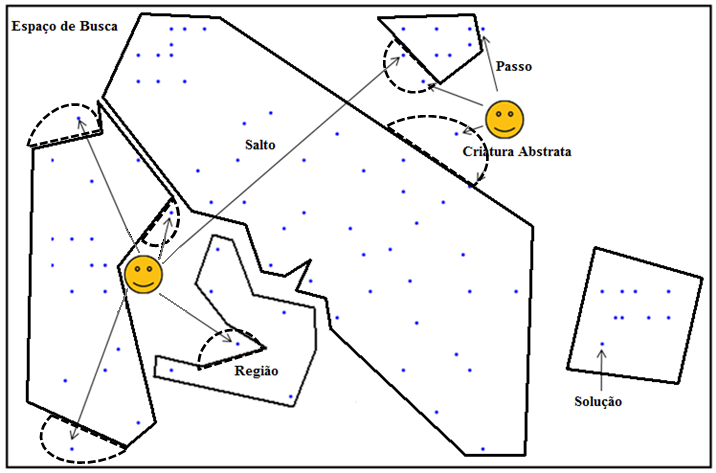
\includegraphics[scale=0.45]{imagens/bimasco-saliba.png}
    \fonte{\citeonline{saliba2010}}
    \label{fig:bimasco_saliba}
\end{figure}


Neste ponto é necessário ressaltar que apesar do autor prever a divisão do espaço em regiões, e introduzir um comportamento básico pra elas, ele não entra em detalhes do seu funcionamento e também não as implementa.

Os \textbf{agentes} são formados pela união de vários componentes. Entre os principais estão os mecanismos de aprendizagem, componentes emocionais, efetores e sensores. Além disso, encapsulam as heurísticas e meta-heurísticas e interagem com esse espaço de busca, produzindo e consumindo soluções do mundo, aprendendo a buscar melhores soluções. Cada componente do agente executava em uma \textit{thread} separada, que se comunicavam por troca de mensagens, por meio de uma área de memória compartilhada, chamada de \textit{Interoceptive Pool}. A \autoref{fig:interoceptive_pool_saliba} ilustra os diversos componentes que compõe o agente, incluindo os sensores, efetores, componentes do sistema nervoso artificial, bem como a comunicação entre eles por meio de memória compartilhada.

\begin{figure}
    \centering
    \caption{Esquema dos componentes internos do agente, os estímulos, ou mensagens que eles trocam entre si, e o \textit{Interoceptive Pool}, memória compartilhada utilizada para a troca de mensagens}
    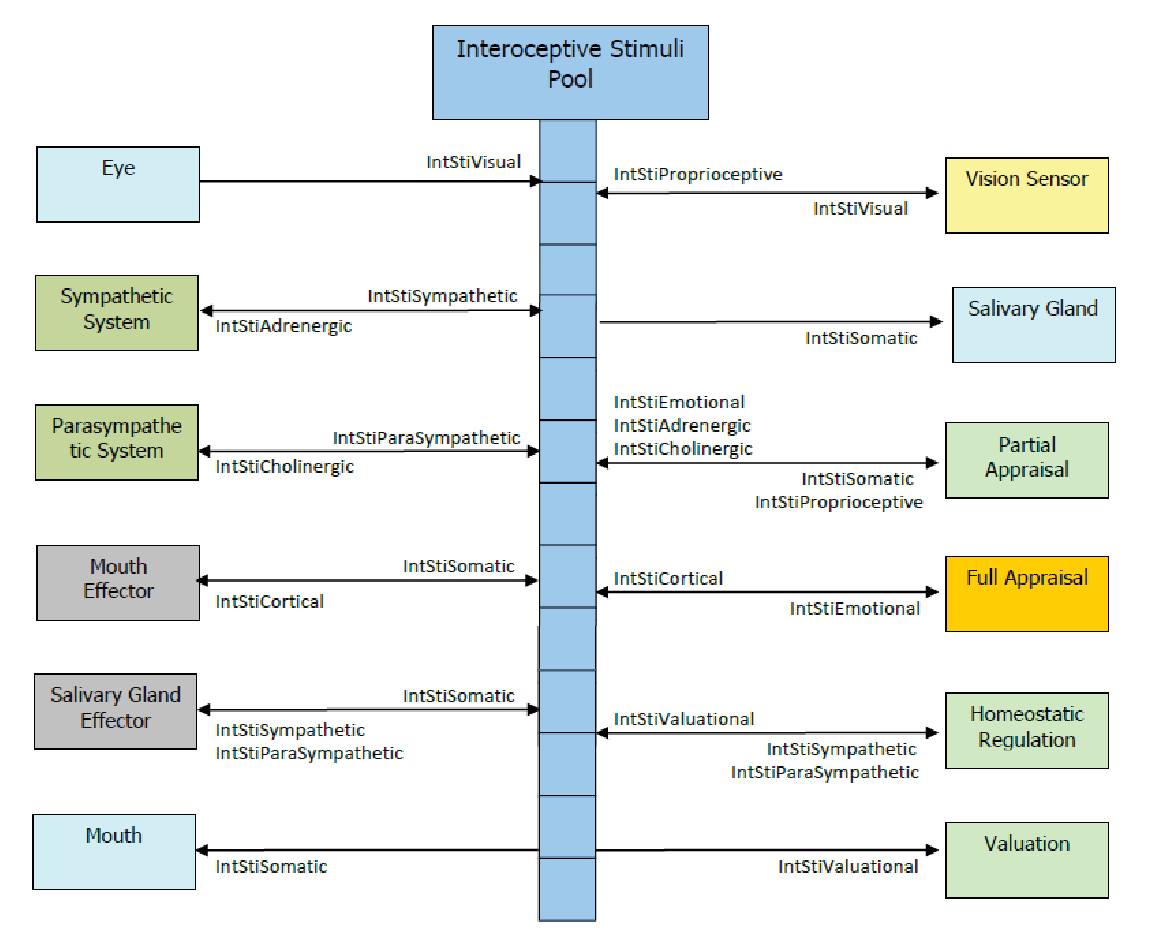
\includegraphics[scale=0.6]{imagens/interoceptive-pool-saliba.eps}
    \fonte{\citeonline{saliba2010}}
    \label{fig:interoceptive_pool_saliba}
\end{figure}

O objetivo é que os agentes aprendam a encontrar boas soluções para um problema de otimização baseado nessa interação e na colaboração entre eles. A interação com o espaço de busca acontece também por meio de troca de mensagens,  baseada em compartilhamento de estado, por meio do \textit{Environmental Pool}. A \autoref{fig:bimasco_env_pool} ilustra o funcionamento do \textit{Environmental Pool}, que é basicamente uma lista compartilhada onde agentes e regiões podem colocar mensagens endereçadas a outras entidades, bem como consultar periodicamente se há mensagens endereçadas para si.

\begin{figure}
    \centering
    \caption{Mensagenes trocadas entre agentes e regiões através do \textit{Environmental Pool}.}
    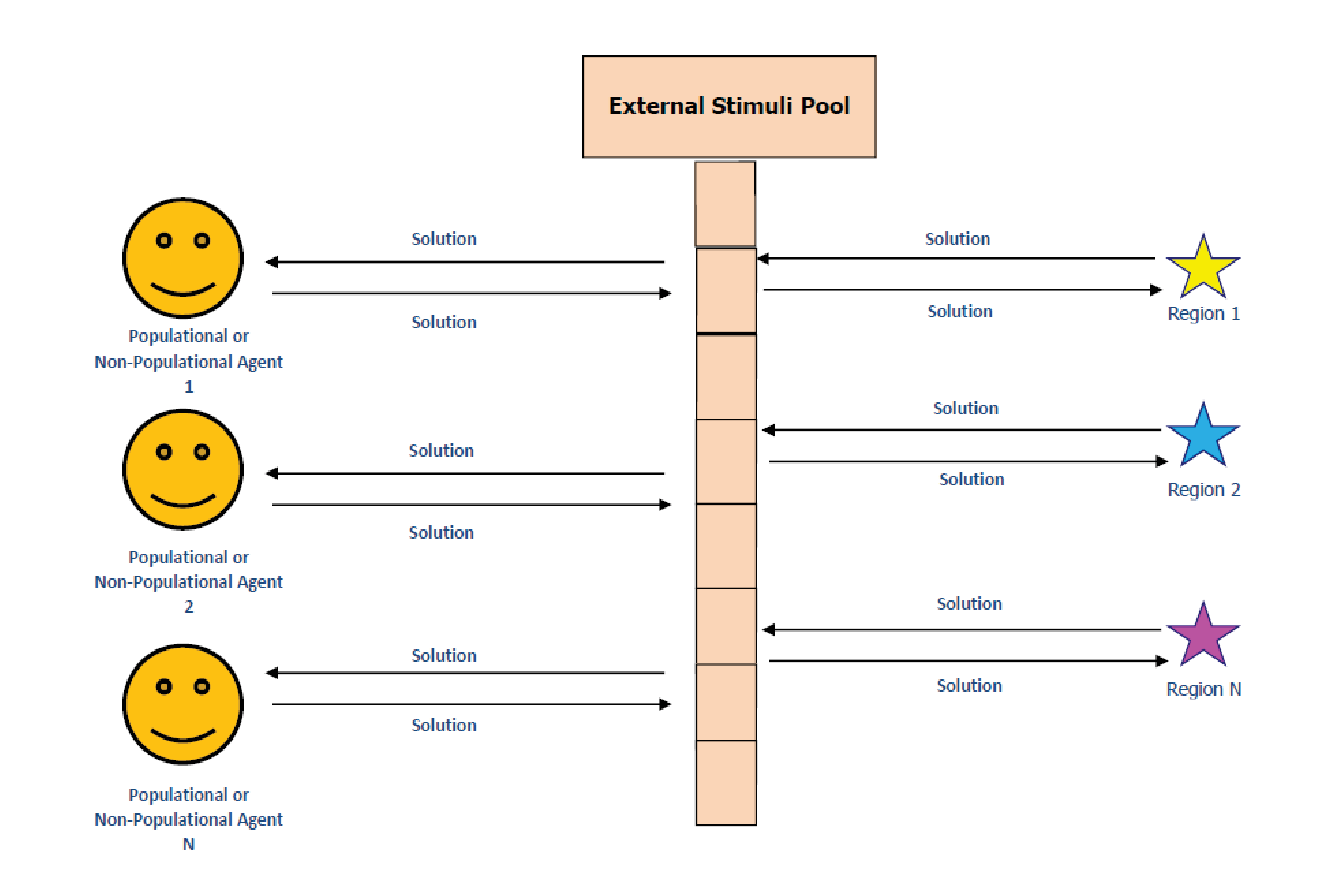
\includegraphics[scale=0.5]{imagens/external-pool-saliba.eps}
    \fonte{\citeonline{saliba2010}}
    \label{fig:bimasco_env_pool}
\end{figure}

Os agentes podem ser divididos em construtores, populacionais e não-populacionais, baseado no funcionamento de cada um e em suas interações com o espaço de busca. Um agente construtor, por exemplo, não precisa consumir nenhuma solução inicial do mundo, pois constrói uma solução, elemento a elemento, baseado em alguma estratégia, que pode ser gulosa ou randômica. Um agente populacional encapsula uma estratégia de busca baseada em populações, \textit{e.g.}, um algoritmo genético, e por isso necessita de um conjunto inicial de soluções para funcionar. Assim, o agente busca soluções iniciais no espaço de busca, processa e entrega um conjunto melhorado de soluções ao mundo. Agentes não-populacionais são aqueles que realizam buscas locais, e necessitam de uma solução para iniciar a busca, produzindo uma solução que pode ser um ótimo local, ou um ótimo global. 

Nesta primeira versão da arquitetura estavam presentes algumas estratégias de busca conhecidas da literatura, são elas: a heurística construtiva GRASP (\textit{Greedy Randomized Adaptive Search Procedure}), os métodos de busca local ILS (\textit{Iterated Local Search}) e VNS (\textit{Variable Neighborhood Search}) e a meta-heurística populacional GA (\textit{Genetic Algorithm}). Para avaliar o funcionamento da sua arquitetura, \citeonline{saliba2010} executou alguns experimentos com instâncias do Problema de Roteamento de Veículos com Janela de Tempo (PRVJT), propostas por \citeonline{solomon1987}, e compara os seus resultados com os da arquitetura AMAM. Entretanto, ele não apresenta um procedimento experimental adequado para um sistema não-determinístico, como é o BIMASCO, e muito menos uma análise estatística rigorosa, prejudicando uma comparação entre as arquiteturas. 

Apesar de \citeonline{saliba2010} ter projetado o BIMASCO para ser facilmente extensível e flexível tanto para os métodos de busca quanto para os problemas, foi somente no trabalho de \citeonline{denise2014} que a arquitetura foi estendida para que as heurísticas fossem completamente independentes da representação e dados dos problemas. Para tanto a autora tornou as soluções genéricas quanto ao tipo de dado, podendo ele ser booleano, inteiro ou real. Também criou artefatos de software para abstrair as estratégias que atuam sobre as soluções e que são comuns a vários algoritmos de busca. Esses artefatos foram nomeados \textbf{movimentos}, que consistem na alteração de uma posição do vetor no espaço de objetivos, levanto a solução para um vizinho próximo, e  \textbf{modificadores}, que podem ser vistos como um conjunto de movimentos. Um movimento ou um modificador pode ser aplicado a uma ou mais soluções, e foram implementados para as principais heurísticas e para os tipos de dados propostos. A autora deixa claro que "[...]  os modificadores são totalmente dependentes do tipo de
representação do problema e não do problema em questão" \cite{denise2014}. 

Nesta versão do BIMASCO novos problemas foram adicionados à arquitetura, a saber: o problema da otimização irrestrita de função real,  da diversidade máxima, da mochila e o problema da partição binária. Foi adicionada a heurística \textit{Simulated Anealing} e as heurísticas existentes foram adaptadas para funcionarem de maneira independente da representação das soluções, utilizando somente os movimentos e modificadores propostos. Em seguida, foram apresentados três conjuntos de experimentos para validar a generalização da arquitetura executando diferentes combinações de problemas e heurísticas, bem como o correto funcionamento das heurísticas. A arquitetura alcançou bons resultados para a maioria dos problemas, apesar do efeito dos mecanismos de aprendizagem não ter sido avaliado, e a implementação dos comportamentos para as regiões foi elencada somente na secção de trabalhos futuros. 

Dando prosseguimento no trabalho de \citeonline{denise2014}, \citeonline{marcus2015} simplificou a arquitetura, removendo a maioria dos componentes herdados da arquitetura ARTÍFICE que oneravam a simulação, tornando-a mais lenta e menos competitiva que outras arquiteturas. Deste modo, o autor propõe um mecanismo simplificado baseado em aprendizagem  por reforço, um protocolo de comunicação entre os agentes, e uma primeira implementação da dinâmica das regiões. Nesta nova versão, os agentes passam a ser compostos somente de 3 \textit{threads}: um componente sensor, efetor e o \textit{Evaluator}. Por meio do componente sensor, os agentes podem solicitar soluções a outros agentes e às regiões, com uma probabilidade associada. Essa probabilidade é alterada a medida que o agente interage com o mundo e produz soluções melhores do que as produzidas anteriormente. Essas soluções são avaliadas pelo \textit{Evaluator}, que altera as probabilidades na memória do agente. 

Para escolher, dentre os agentes e regiões na memória, de qual solicitar soluções, o algoritmo funciona basicamente em duas etapas. Inicialmente, ele faz uma roleta entre todos os agentes e reserva uma fatia dessa roleta para as regiões. Caso algum agente seja sorteado, é enviado uma mensagem diretamente pra ele. Mas caso a escolha recaia sobre as regiões, é feita uma nova roleta as entre regiões e o agente pede soluções para a região escolhida. O agente utiliza as soluções recebidas para executar a meta-heurística que encapsula e produzir novas soluções, que retornam para o mundo.O componente efetor é responsável por enviar essas soluções produzidas para uma região. Entretanto, \citeonline{marcus2015} não dá detalhes sobre como um agente escolhe para qual região enviar essas novas soluções. 

A estratégia proposta para a fusão e fissão das regiões ficou baseada na análise da variância e covariância dos valores de função objetivo dos conjuntos de soluções que formam as regiões. Para se dividir, uma região verifica se a variância da função objetivo está acima de um limiar que é dado como parâmetro no arquivo de configuração da simulação. Se a $\sigma^{2}$ for maior que este parâmetro, a  região se particiona em 3 novas regiões contendo as soluções com valor de função objetivo que estavam abaixo de $\mu - \sigma$, entre $\mu - \sigma$ e $\mu + \sigma$ e as que estavam acima de $\mu + \sigma$. Para duas regiões fazerem fusão, a covariância entre as duas tem de ser maior que um limiar, que também é um parâmetro da configuração da arquitetura. É importante observar que o autor não mostra detalhadamente como essa analise é feita. Por exemplo, a fórmula da covariância entre duas amostras $X$ e $Y$ de tamanho $N$ com médias $\overline{X}$ e $\overline{Y}$ pode ser escrita da seguinte maneira:
\begin{equation}
\label{eq:cov}
    cov(X,Y) = \sum_{i=1}^{i<N}\frac{(x_i - \overline{X})(y_i - \overline{Y})}{N - 1} 
\end{equation} 
Aplicando a \autoref{eq:cov} ao contexto da fusão entre duas regiões, seria necessário que ambas tivessem o mesmo número $N$ de soluções. Entretanto, pela característica estocástica do sistema, muito raramente duas regiões terão o mesmo número de soluções. Esse caso de borda não foi abordado na modelagem do autor, muito menos nos experimentos realizados. 

Neste trabalho foram executadas 5 baterias de experimentos dos quais 4 estavam voltados para avaliar o desempenho da arquitetura com e sem colaboração entre os agentes (permitindo ou não que os agentes troquem soluções) e 1 voltado para avaliar o efeito de utilizar uma ou mais regiões na simulação, alterando somente os limiares de fusão e fissão. Na maioria dos experimentos foi observado que a interação entre os agentes e a aprendizagem favorecem a busca por melhores soluções. No entanto, não foi possível tirar alguma conclusão sobre o efeito da separação do espaço em regiões para o funcionamento da arquitetura.

A falta de experimentos em larga escala com a arquitetura BIMASCO motivou \citeonline{pacheco} a propor uma nova implementação da arquitetura, desta vez baseada num modelo de concorrência mais moderno, denominado modelo de atores. Proposto inicialmente por \citeonline{hewitt1973}, o modelo de atores se contrapõe ao modelo de concorrência por \textit{threads} e compartilhamento de estado. Os atores, unidades básicas de computação, não compartilham o estado interno e se comunicam somente por meio de troca de mensagens assíncronas. O autor utilizou como ferramenta o \textit{framework Akka}\footnote{https://akka.io/}, uma implementação do modelo de atores para linguagens baseadas na JVM, como o Java. 

A mudança de paradigma oferece à arquitetura remodelada a vantagem de poder escalar horizontalmente, como um sistema distribuído, o que inclusive leva à mudança do nome do projeto, que deixa de se chamar BIMASCO e passa a se chamar D-Optimas. Os agentes e regiões também foram reduzidos a um único ator que executa a regra de negócio principal, mas sem perderem as suas funcionalidades descritas nos trabalhos anteriores. 

A \autoref{fig:d_optimas_pacheco} ilustra a hierarquia de atores proposta por \citeonline{pacheco}. O ator \textit{/user} faz parte do \textit{toolkit Akka} e supervisiona todos os atores criados pelo programa, os atores \textit{/agents} e \textit{/regions} criam, supervisionam e finalizam a execução de agentes e regiões respectivamente. O ator \textit{/reaper} é o responsável por finalizar a simulação quando atingido o critério de parada. Uma maneira possível de executar essa arquitetura em um \textit{cluster}\footnote{No contexto da computação distribuída, um \textit{cluster} nada mais é do que um conjunto de computadores conectados através de uma rede, os quais podem ser chamados de membros, nós, \textit{workers}, \textit{slaves}, a depender do autor. O presente trabalho utiliza o termo nó, por não haver qualquer distinção entre o papel dos computadores em si. } seria alocar o ator \textit{/agents} em uma máquina com o endereço \textit{192.168.0.1}, e o \textit{/regions} no computador endereçado no IP \textit{192.168.0.2}, ambos na porta \textit{2551}. Para o agente \textit{a1} se comunicar com a região \textit{r1} é necessário que ele saiba o endereço completo do agente, que seria \textit{akka://192.168.0.2:2551/user/regions/r1}.

\begin{figure}
    \centering
    \caption{Hierarquia de atores proposta para a arquitetura D-Optimas.}
    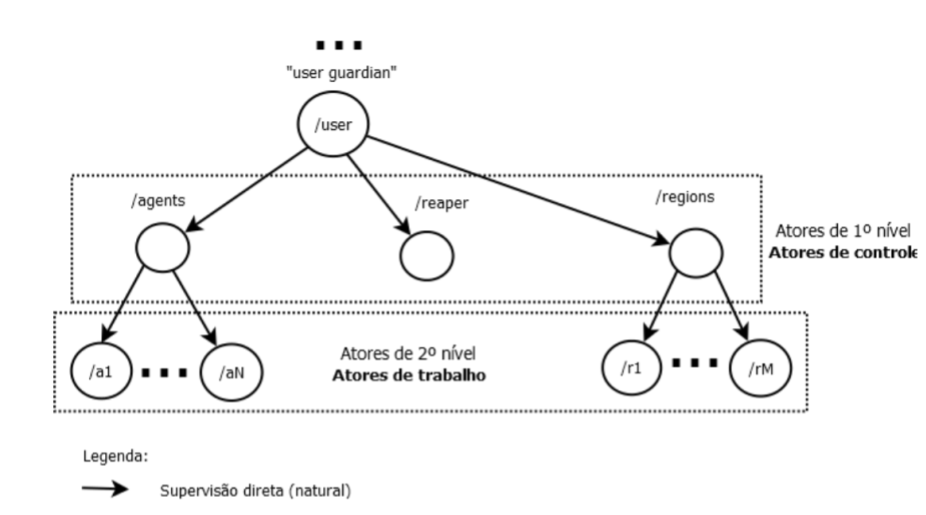
\includegraphics[scale=0.4]{imagens/d-optimas-pacheco.png}
    \fonte{\citeonline{pacheco}}
    \label{fig:d_optimas_pacheco}
\end{figure}

O autor apresenta dois experimentos para avaliar o resultado da mudança: o primeiro, para verificar a corretude do sistema e certificar de que a mudança de paradigma não alterou nenhuma funcionalidade até aqui desenvolvida, e um segundo que avaliou a escalabilidade da arquitetura, coletando dados de 30 execuções com mais de 1000 agentes. Entretanto, o segundo e principal experimento não avaliou o funcionamento da arquitetura em mais de 2 nós, não exibindo nenhum dado sobre a escalabilidade horizontal do sistema.

\section{Considerações Finais}
O presente capitulo se dedicou a fazer uma revisão da literatura de arquiteturas multi-agentes para otimização. Foram apresentadas alguns trabalhos que compartilham características importantes, baseado principalmente na revisão mais recente realizada por \citeonline{silva2018}. Entre essas arquiteturas, foi apresentada também a arquitetura AMAM, proposta por \citeonline{silva2019} e por fim, a arquitetura D-Optimas. As suas principais características, resultado de diversas contribuições ao longo dos últimos 10 anos, foram exploradas, bem como suas eventuais deficiências, que se convertem em boas oportunidades de trabalho. O capitulo seguinte apresenta os esforços que foram feitos no presente trabalho para reparar essas deficiências e estender o projeto. 	% Descrição do Problema
 \chapter{Metodologia}
\label{chap:metodologia}
% origem do d-optimas no bimasco 
% retomar os objetivos do trabalho: criar um sistema resiliente, 
O capítulo anterior apresentou algumas arquiteturas e \textit{frameworks} para resolução de problemas de otimização que podem ser executadas em um \textit{cluster}. Entre elas, se destaca a arquitetura D-Optimas, baseada no sistema de atores. Do ponto de vista de sistemas distribuídos, essa arquitetura apresenta algumas dificuldades para executá-la em um \textit{cluster} com mais de dois nós. Além disso, é possível observar também alguns aspectos da modelagem que tornam a configuração da arquitetura muito acoplada ao problema de otimização, principalmente no que diz respeito aos parâmetros das regiões.

Deste modo, o presente trabalho se dedica a propor melhorias na arquitetura D-Optimas, a fim de tornar o comportamento das regiões menos dependente de algum conhecimento prévio do problema e também possibilitar a escalabilidade horizontal da arquitetura. O presente capítulo é dedicado a expor a metodologia utilizada para atingir os objetivos propostos no \autoref{chap:introducao}. A próxima seção apresenta as hipóteses que guiam este trabalho. Em seguida, na \autoref{sec:metodo} é apresentado o método utilizado para por as hipóteses à prova. A \autoref{sec:premissas} apresenta as premissas que podem ser assumidas no decorrer da metodologia, e por fim, a \autoref{sec:experimentos} apresenta os experimentos que serão executados para verificar as hipóteses.


\section{Hipóteses}
\label{sec:hipoteses}
% retomar as hipoteses dos trabalhos anteriores
Dentre os trabalhos que envolveram a arquitetura D-Optimas e sua antecessora, o Bimasco, se destacam as contribuições mais recentes de \citeonline{marcus2015} e \citeonline{pacheco}. As hipóteses levantadas e testadas por \citeonline{marcus2015} foram de que a diversidade de agentes poderia favorecer a exploração do espaço de busca e que a segregação das soluções em regiões em conjunto com um mecanismo de aprendizagem levaria os agentes a buscarem soluções de melhor qualidade. Por sua vez, \citeonline{pacheco} levantou a hipótese de que a mudança para o modelo de atores permitiria que a arquitetura escalasse de maneira vertical, em um único computador, e de maneira horizontal, ao longo de um \textit{cluster}. De maneira mais geral, a hipótese que motiva a construção da arquitetura é de que nenhuma meta-heurística particular é capaz de encontrar bons resultados para todos os tipos de problemas, porém uma combinação adequada delas poderia gerar resultados melhores. 

% retomar o meu problema
Sendo assim, torna-se necessário conduzir um estudo mais  detalhado do comportamento da arquitetura ao longo de uma simulação, com a presença de uma maior diversidade de meta-heurísticas. É também necessário verificar o desempenho da D-Optimas em um \textit{cluster} com vários computadores, onde a influência da rede é crítica e onde a escalabilidade horizontal poderia ser melhor verificada. Além disso, a implementação de um conjunto muito restrito de meta-heurísticas impediu uma investigação mais detalhada do efeito da diversidade no processo de busca. Espera-se que, corrigidas as falhas discutidas no capítulo anterior e adicionando novas meta-heurísticas, seja possível avaliar com maior robustez algumas destas hipóteses. 

% introduzir a minha hipótese
A primeira hipótese que se pode formular no presente trabalho é que a versão da arquitetura produzida exibe um comportamento convergente em torno do valor conhecido da função objetivo dos problemas propostos na literatura. A segunda hipótese formulada é que o aumento do número de nós não acarreta em perda de desempenho ou diminuição da taxa de convergência da arquitetura. E por fim, é possível revisitar a hipótese levantada por \citeonline{marcus2015},de que, ao inserir diversidade de estratégias
de busca, combinada com um sistema de memória e um mecanismo de colaboração entre
os agentes, a arquitetura é capaz de produzir soluções de melhor qualidade para diferentes problemas.


\section{Método}
\label{sec:metodo}

Como já foi dito, o objetivo do presente trabalho é construir uma nova versão da arquitetura  D-Optimas, baseado na versão proposta por \citeonline{pacheco}. Este sistema multi-agentes deve ser construído sem um controle central, utilizando técnicas e ferramentas de sistemas distribuídos, que permitam a sua execução em um \textit{cluster} com um número arbitrário de nós. Nesta nova versão, as regiões devem funcionar de maneira independente dos dados do problema objeto de estudo, necessitando o mínimo de conhecimento prévio acerca dele para configurar a arquitetura. Também se pretende adicionar novas meta-heurísticas à arquitetura, adaptando-as para funcionar num contexto distribuído, a fim de poder obter resultados confiáveis para avaliar o desempenho do sistema em diferentes problemas de otimização. 

Posto esse objetivo e as hipóteses levantadas na seção anterior, a metodologia estabelecida para atingir os objetivos e por as hipóteses à prova consiste em, inicialmente, compreender a atual versão da arquitetura, desenvolvida por \citeonline{pacheco} sobre o \textit{toolkit akka}, e verificar quais pontos têm dificultado sua execução em um \textit{cluster} com mais de dois nós. 

Para suplantar essas dificuldades, é necessário, em seguida, estudar os recursos do \textit{toolkit akka}, em especial, as ferramentas que compõem o \textit{akka-cluster}, o qual implementa todas as primitivas e recursos para desenvolvimento de um sistema distribuído. A biblioteca \textit{akka-cluster} foi escolhida em detrimento de várias outras alternativas pois a última versão da arquitetura já está implementada no modelo de atores, adotado na D-Optimas. Assim, adotar esta implementação dos algoritmos clássicos de sistemas distribuídos, tais como descobrimento de nós e eleição de líder, parece uma escolha natural e que leva ao menor retrabalho.

Após compreender a arquitetura D-Optimas e as ferramentas necessárias para a implementação de um sistema distribuído, é necessário refatorar a arquitetura para incluir os recursos do \textit{akka-cluster}. As modificações nos protocolos de funcionamento serão inevitáveis, pois apesar de alguns atores supervisores já existirem, eles não foram preparados para chegar a um consenso sobre, por exemplo, para qual região uma solução deveria ir em um sistema distribuído. Nesta nova versão da arquitetura, atores supervisores do mesmo tipo precisarão manter uma comunicação frequente e um estado distribuído da aplicação, permitindo ao sistema como um todo ser resiliente a falhas.

Para além de refatorar a comunicação entre os atores supervisores, será necessário detalhar e implementar o funcionamento das regiões em concordância com os objetivos aqui propostos. A primeira versão das regiões implementada por \citeonline{marcus2015} estava fortemente amarrada a um conhecimento prévio do problema. O que se propõe aqui é aprimorar a implementação, desvinculando-a dos dados do problema, e estudar o efeito macro dos comportamentos de fissão e fusão no comportamento/resultados gerados pela arquitetura. Além disto, \citeonline{marcus2015} apontou como uma oportunidade de trabalho futuro a inserção de novas meta-heurísticas a arquitetura, uma vez que a escassez delas pode ter influenciado na performance de seus resultados. Assim, é necessário revisar a literatura, encontrar meta-heurísticas que sejam relevantes para este trabalho, estudar o seu funcionamento, adaptá-las ao contexto de um sistema multi-agente genérico no que diz respeito à representação dos problemas, e implementá-las neste sistema.

Para validar as hipóteses levantadas na seção anterior, experimentos serão executados e dados serão coletados, tratados e analisados. Todavia, num sistema distribuído e assíncrono, que opera por meio de troca de mensagens, a coleta de dados confiável, que preserva a sequência temporal dos mesmos está longe de ser tarefa trivial, como é em outros cenários. Neste contexto, será necessário propor e implementar um sistema de persistência e coleta de dados adequado à um sistema distribuído. Neste tipo de sistema as entidades podem e, de fato migram de um nó para outro. Portanto, manter ativa e funcional uma conexão com um banco de dados centralizado, e muitas das vezes remoto, representa não apenas uma tarefa árdua, como também um possível gargalo/ponto único de falha. Além disto, como a escrita no banco de dados é uma operação muito mais dominante na D-Optimas em comparação com a leitura, é possível abrir mão dos princípios de ACID\footnote{Sigla  para Atomicidade, Consistência, Isolamento e Durabilidade. Estas quatro propriedades são fortemente garantidas em bancos de dados relacionais, o que permite o desenvolvimento de aplicações confiáveis para o usuário final. No contexto do desenvolvimento de sistemas distribuídos, é comum abandonar a premissa de consistência e adotar uma consistência eventual, onde, em algum momento no tempo, todas as instâncias do banco de dados terão o mesmo conjunto de dados.} e utilizar um banco de dados distribuído não-SQL. Ao longo da execução, os agentes e regiões escrevem no banco de dados os eventos relevantes (por exemplo, a produção ou recebimento de uma nova solução, uma operação de fusão ou fissão), e ao final da execução, esses dados são extraídos pela arquitetura, recebendo neste ponto um primeiro tratamento, como por exemplo, a ordenação, agrupamento e remoção de eventuais dados duplicados. 

Ao final deste tratamento, os dados são salvos em um conjunto de arquivos texto do tipo \textit{csv}. Para cada série de dados extraída, e para cada entidade, um novo arquivo é criado, \textit{i.e}, há pelo menos um arquivo para cada região/agente na simulação. Os dados extraídos são: as soluções produzidas por cada agente e o intervalo de tempo para produzir cada solução, as soluções recebidas por cada região, os parâmetros estatísticos das regiões, a melhor solução de cada região, a melhor solução global, as estatísticas globais e as mensagens trocadas. Todos esses dados são séries temporais discretas. Quanto ao sistema de banco de dados, nas versões anteriores era utilizado o Sistema Gerenciador de Banco de Dados (SGDB) \textbf{PostgreSQL}. Para a versão atual foi escolhido o \textbf{Cassandra}\footnote{https://cassandra.apache.org/}. Essa escolha se deu pois a biblioteca \textit{akka-cluster} já possui um \textit{plugin} para \textit{journaling} e persistência do estado distribuído da aplicação, e também por ser um SGDB adequado à implementação de sistemas distribuídos. Por simplicidade de configuração e manutenção, foi feita a opção por utilizar um único sistema de banco de dados.

% não entendi as duas últimas frases do parágrafo. Explicar melhor!!

Para executar a arquitetura no \textit{HPC} do CEFET-MG é necessário preparar um ambiente que é complexo, alocar os recursos computacionais, prover arquivos de configuração para o banco de dados, limpar os arquivos temporários que permaneceram nos nós de execuções passadas, iniciar e popular o banco com as tabelas, executar o experimento, extrair esses dados e, por fim, copiar os \textit{logs} da execução. Sobretudo, é necessário garantir que todo experimento inicie sob as mesmas condições, de modo a evitar qualquer viés na coleta dos dados. Para configurar o ambiente, executar e armazenar os dados é necessário produzir uma série de \textit{scripts} de configuração que seguem o padrão do escalonador do \textit{HPC}, no caso do CEFET-MG, o SLURM.

Uma vez alcançados todos estes passos que dizem respeito ao desenvolvimento tecnológico do problema proposto, há que efetivamente executar a bateria de experimentos propostos para por à prova cada uma das hipóteses. Antes disso é necessário formular as hipóteses estatísticas e verificar as premissas para cada um dos conjuntos de dados. Baseado nas premissas, é possível escolher os testes estatísticos apropriados (paramétricos ou não), o nível de significância, o poder do teste e o tamanho da amostra. Baseado nesse planejamento é possível executar os experimentos, coletar e caracterizar os dados utilizando o arcabouço da estatística descritiva e, finalmente, submeter cada uma das hipótese formuladas a um teste estatístico visando refutá-las. 

\section{Premissas}
\label{sec:premissas}
% as distribuições dos valores de  funções objetivos não são normais
Nos experimentos conduzidos por  \citeonline{marcus2015} o efeito da cooperação entre os agentes foi avaliado. O autor comparou os melhores valores de função objetivo que a arquitetura produziu em 30 execuções em que os agentes não colaboravam com outras 30 execuções em que a colaboração estava habilitada. \citeonline{pacheco} repetiu parte desses experimentos e realizou comparações para se certificar que as alterações no modelo de comunicação da arquitetura não alterariam o seu comportamento. Ambos os autores se limitaram a fazer comparações visuais utilizando o \textit{boxplot}, e por isso não fizeram nenhum teste de hipótese sobre a amostra. Entretanto, por mera inspeção destes mesmos \textit{boxplot}, é possível perceber que os valores de função objetivo não seguem uma distribuição normal. Portanto, não se pode assumir normalidade da amostra de valores ótimos obtidos pela arquitetura.

% em contrapartida, a amostragem dos tempos de latência podem ser tratados como normais, pelo teorema do limite central
\citeonline{pacheco} avaliou também a escalabilidade da arquitetura, e verificou que utilizando 2 nós no \textit{cluster}, é possível aumentar o número de agentes e observar um aumento proporcional da quantidade de soluções obtidas em um mesmo intervalo de tempo. Entretanto, essa escalabilidade não foi avaliada quando outros nós são adicionados à simulação. Espera-se que o aumento do número de nós possa intensificar a comunicação pela rede, gerando algum atraso nas mensagens. Como será avaliada a latência média, espera-se que a distribuição das médias das latências siga uma distribuição normal pelo teorema do limite central.

% uma execução da arquitetura no cluster de alto desempenho do cefetmg não infuência as próximas execuções
Ao executar uma bateria de experimentos no \textit{HPC} do CEFET-MG, espera-se que uma execução sempre inicie em um ambiente limpo, sem influência de execuções passadas. Parte disso é garantido pelo próprio \textit{script} de execução, que remove todos os arquivos temporários antes de iniciar uma nova execução, e também inicia o banco de dados em um estado inicial.  

% as execuções são numa rede isolada, num ambiente controlado, sofrendo influências somente das tarefas gerenciais do cluster
Dado que as execuções são realizadas em um ambiente isolado, gerenciadas por um escalonador de recursos (no caso do \textit{cluster} do CEFET-MG, é utilizado o SLURM\footnote{https://slurm.schedmd.com/}), é possível presumir que outras tarefas não irão influenciar a execução do D-Optimas, pois não haverá competição por recursos computacionais, tais como memória e processador. Em outras palavras, dado que o \textit{script} da simulação reserva uma certa quantidade de núcleos de processamento e memória, uma execução iniciará e terminará com os mesmos recursos, não sendo escalonada com outras tarefas de outros usuários, dividindo espaço somente com as tarefas gerenciais do escalonador e do sistema operacional. 

% as únicas mensagens que trafegam na rede com alguma relevância são as do d-optimas
Os experimentos serão executados em uma fila do \textit{HPC} do CEFET-MG reservada à pesquisa do Laboratório de Sistemas Inteligentes do CEFET-MG. Os computadores dessa fila estão isolados da rede do restante do \textit{cluster}, portanto, a última premissa que este trabalho assume é que as únicas mensagens que trafegarão na rede com alguma relevância serão as da arquitetura D-Optimas. Além disso, fez-se o melhor esforço para minimizar outros tipos de comunicação (por exemplo, as do sistema de arquivos, que utiliza o protocolo NFS). Assume-se que as mensagens de gerenciamento e monitoramento do escalonador trafegam na mesma rede em que trafegam as mensagens específicas da D-Optimas, não obstante, elas não influenciam de maneira crítica o resultado dos experimentos. Isso é possível de ser verificado utilizando o utilitário de monitoramento do \textit{HPC} do CEFET-MG, o \textbf{Ganglia}\footnote{É possível acessa-lo na rede interna do CEFET-MG através do endereço http://cluster.decom.cefetmg.br}. Nele é possível verificar que o tráfego na rede quando o super-computador está ocioso é mínimo. Além disso, todo o tráfego é direcionado ao nó mestre do \textit{HPC}, que não é diretamente utilizado durante as simulações da arquitetura D-Optimas.

% os relógios das máquinas estão em sincronia
Por fim, é possível presumir que os relógios das máquinas estejam sincronizados. Essa premissa está baseada no fato de que no \textit{HPC} do CEFET-MG os nós estão configurados para sincronizar os relógios com o nó mestre utilizando o \textit{NTP} (\textit{Network Time Protocol}). Eventualmente, pode haver algum atraso entre os relógios de duas máquinas particulares, mas espera-se que esse efeito não seja significante, uma vez que os resultados dos experimentos serão amostrados considerando as médias das latências. 

\section{Experimentos}
\label{sec:experimentos}
Para colocar à prova as hipóteses propostas neste trabalho,  três experimentos computacionais foram previstos. O primeiro visa avaliar a corretude da arquitetura, verificando se as alterações no comportamento das regiões e na comunicação entre os atores supervisores produzem um comportamento de convergência em torno dos valores conhecidos de função objetivo para cada problema. Em outras palavras, deseja-se verificar a hipótese nula de que a média populacional dos valores de função objetivo obtidos pela arquitetura é igual ao valor ótimo conhecido pela literatura, contra a hipótese alternativa de que os valores de função objetivo  obtidos pela  atual versão da arquitetura sejam  diferentes dos valores conhecidos da literatura. 

Para isso, será necessário utilizar um teste de hipótese não paramétrico para uma amostra, uma vez que não é possível assumir normalidade dos valores de função objetivo obtidos pela arquitetura. Neste ponto há uma dificuldade significativa, pois é sabido que o poder dos testes não paramétricos é menor, o que requer amostras maiores, e pela complexidade tecnológica da arquitetura D-Optimas, coletar amostras grandes é muito custoso, ainda que utilizando um \textit{HPC}. 

Além de avaliar o correto comportamento da arquitetura, é necessário avaliar a escalabilidade da arquitetura ao longo de um \textit{cluster}, executando-a em vários nós ao mesmo tempo. Espera-se que ao aumentar a quantidade de nós na simulação, preservando o número de agentes e o limite de regiões, a latência não aumente de maneira significante, bem como não prejudique a quantidade de soluções geradas da arquitetura e nem afete a sua qualidade. Dito de outra maneira, é necessário fazer duas análises de variância para um fator. Deseja-se avaliar a média da latência das trocas de mensagens e a quantidade de soluções produzidas por intervalo de tempo, para diferentes valores do fator número de nós em que a simulação executa. 

Neste experimento o resultado esperado para o modelo proposto de comunicação entre os atores supervisores e os agentes é que não haja diferença estatisticamente significante para os diferentes níveis do fator número de nós no \textit{cluster}, \textit{i.e.}, não há diferença entre executar a arquitetura com dois, três ou mais nós. Um resultado positivo neste quesito daria um indício da resiliência da arquitetura a diferentes cargas e do seu potencial de escalabilidade. 

Por fim, dadas as novas meta-heurísticas que foram adicionadas na atual versão, procura-se verificar, com um número grande de agentes com diferentes estratégias de busca, se os resultados encontrados são melhores que os obtidos por \citeonline{marcus2015}. Em outras palavras, deseja-se verificar a hipótese nula de que a média dos resultados da arquitetura com várias heurísticas e diferentes configurações é melhor do que a média dos resultados com pouca diversidade de estratégias de busca.

Novamente, há um elemento expressivo de estocasticidade neste experimento que tem origem em diferentes fontes. Entre elas destaca-se o fato de cada agente iniciar com um gerador de números aleatórios diferentes, que é utilizado para a tomada de decisão dos algoritmos; as regiões se agruparem de maneira não-determinística; e finalmente o conjunto de soluções dos algoritmos populacionais não ter sido gerado aleatoriamente, mas escolhido de uma ou mais regiões particulares do espaço de busca. Esses elementos de aleatoriedade dificultam a identificação da função de densidade de probabilidade dos valores de função objetivo obtidos pela arquitetura, e portanto impedem o uso de testes paramétricos. Esses fatores levam à necessidade de se coletar amostras grandes, por longos períodos de tempo, para avaliar a arquitetura com um valor de significância razoável (abaixo de 5\%).

\section{Considerações Finais}
O presente capítulo se dedicou a expor a metodologia científica proposta para a realização deste trabalho. Foram apresentadas três hipóteses que fundamentam esse projeto de pesquisa. Destas três, a última hipótese é a mais relevante do ponto de vista científico. A arquitetura D-Optimas pode ser caracterizada como uma hiper-heurística, um sistema auto-organizável, dotado de um mecanismo de hibridização dinâmica, capaz de gerar combinações e encadeamentos de meta-heurísticas adaptadas às propriedades particulares de cada problema. Além disso, ela é configurável e extensível, permitindo a fácil adição de problemas combinatórios, de otimização irrestrita ou restrita. Além disso, há o fato do sistema ser construído sobre um arcabouço complexo de sistemas distribuídos.  Todos esses fatores tornam a tarefa de estudá-lo, compreendê-lo e testar hipóteses sobre ele um trabalho relevante.

Fez-se aqui também um esforço em levantar as várias premissas que contornam a arquitetura. Um sistema distribuído sofre influência de diversos fatores, incluindo as possíveis falhas na rede, a sincronia entre os relógios dos nós, a carga em cada computador. Todos esses fatores tornam a atividade de replicar e depurar erros bastante complexa. 

Deste modo, o desenvolvimento do trabalho foi feito de maneira criteriosa, testando cada nova funcionalidade, cada meta-heurística separadamente. Algumas destas validações estarão presentes no \autoref{chap:exp_preliminares} e \autoref{chap:exp_diversidade}, ao se fazer a análise da estatística descritiva dos resultados do experimento. O capítulo seguinte se dedicará a apresentar os detalhes do desenvolvimento, principalmente no que diz respeito a nova topologia da arquitetura, adequada para funcionar como um sistema distribuído, e a nova dinâmica das regiões. 			    % Simulação Computacional
 %\include{./02-elementos-textuais/resultadosEsperados}			    % Resultados Esperados
 % -----------------------------------------------------------------------------
%   Arquivo: ./02-elementos-textuais/metodologia.tex
% -----------------------------------------------------------------------------


\chapter{Desenvolvimento}
\label{chap:desenvolvimento}

Algumas arquiteturas para resolução de problemas de otimização foram apresentadas no \autoref{chap:revisao}, em especial as que possuem alguma característica de paralelismo, seja em um único computador, utilizando \textit{multi-threading} ou em um \textit{cluster}, e que sejam baseadas em agentes. Dentre essas se destaca a arquitetura D-Optimas, objeto de estudo do presente trabalho. 

Nesta arquitetura, os agentes encapsulam metaheurísticas e interagem entre si trocando soluções através de um ambiente virtual, buscando aprender nesse ambiente a encontrar soluções de boa qualidade pra qualquer problema de otimização. O ambiente virtual, ou mundo virtual, é composto de soluções que são abrigadas em conjuntos disjuntos, chamados de regiões. O objetivo é que os agentes interajam com as regiões, e não com as soluções diretamente, ''compreendendo'', de maneira genérica, partes do espaço de busca que sejam mais ou menos interessantes. Da mesma forma, espera-se que as regiões possam apresentar uma dinâmica, podendo se fundir ou se particionar, de modo que se adaptem à geometria do espaço de busca de qualquer problema de otimização.   

A arquitetura D-Optimas foi construída baseada no modelo de atores para ser um sistema distribuído. Entretanto, alguns aspectos importantes que são inerentes à um sistema distribuído foram negligenciados na sua primeira versão, principalmente questões relacionadas ao balanceamento de carga, transparência de localidade e resiliência a falhas.

Em um sistema que cresce com o passar do tempo, com agentes produzindo soluções, regiões se fundindo, sendo criadas e se particionando, é importante que o sistema possa criar as agentes e regiões nos nós do \textit{cluster} de maneira equilibrada, de modo a não onerar nenhum nó em particular, fazendo mal uso dos recursos computacionais. A transparência de localidade também deve ser uma característica de um sistema que se propõe a resolver problemas de grande escala, sendo necessário executá-lo em um \textit{cluster} computacional, onde é difícil conhecer previamente os endereços \textit{IPs} das máquinas que executarão o experimento. A resiliência a falhas num sistema distribuído é importante pois falhas na rede são frequentes, um nó pode sair no meio da simulação, e perder as soluções que estavam nele não é aceitável, uma vez que a função objetivo pode ser complexa e custosa para se calcular.
Outro fator importante é a necessidade de uma definição mais precisa da dinâmica das regiões,  que não foi apresentada nos trabalhos anteriores.

Deste modo, neste capítulo a \autoref{sec:topologia} descreve de maneira mais detalhada os conceitos de sistemas distribuídos e os problemas encontrados na arquitetura, bem como apresenta uma nova topologia para os agentes e regiões, baseada na biblioteca \textit{akka-cluster}. A \autoref{sec:dinamica} apresenta os detalhes da dinâmica das regiões, como elas são criadas e quais as condições que permitem à elas fazer fissão e fusão. Por fim, a \autoref{sec:algoritmos} apresenta os algoritmos que foram adicionados à arquitetura, e como esse processo se deu no contexto das abstrações propostas por \citeonline{denise2014} para a generalização de metaheurísticas.

\section{Da topologia do sistema utilizando \textit{akka-cluster}}
\label{sec:topologia}
Como discutido na \autoref{sec:histBimasco}, \citeonline{pacheco} propôs uma remodelagem da arquitetura BIMASCO, utilizando o modelo de atores e o \textit{framework Akka}. Essa remodelagem deu origem à arquitetura D-Optimas, que funciona como um sistema distribuído, podendo ser executada em um \textit{cluster} com dezenas de nós e milhares de agentes. Entretanto, o autor utilizou somente os recursos mais básicos do \textit{framework}, a saber, o recurso de \textit{akka remote}. Este recurso permite que atores que executam em um processo se comuniquem com atores em outro processo.  Entretanto, só a mera comunicação entre processos não é suficiente para caracterizar um sistema como distribuído. Há três propriedades importantes para que um sistema seja considerado distribuído que estão ausentes na arquitetura D-Optimas: tolerância a falhas, balanceamento de carga e transparência de localidade. Os próximos parágrafos argumentam, baseados na literatura, a razão dessas três propriedades serem importantes e apresentam uma solução para esses três problemas, apoiada na biblioteca \textit{akka}.

Segundo \citeonline{tanenbaum}, um sistema distribuído pode ser definido da seguinte maneira:

\begin{quote}
\textit{"A distributed system is a collection of independent computers that appears to its users as a single coherent system"} \cite[p. 2]{tanenbaum}
\end{quote}

Dito isto, o autor ressalta que dois aspectos relevantes dessa definição são a característica autônoma e cooperativa dos componentes do sistema, fazendo com que o usuário, ao lidar com o sistema, perceba-o como um sistema unificado. Este aspecto em especial não está presente na primeira versão do D-Optimas. Um exemplo disso é o caso em que um dos atores supervisores falhe. Neste caso é necessário reiniciar a simulação, o que deixa claro para o usuário que os componentes não colaboram de maneira efetiva. 

Além da falta de resiliência a falhas do sistema, na versão proposta por \citeonline{pacheco} os agentes e regiões precisam saber o endereço físico uns dos outros para poderem se comunicar. É um ponto que também diverge da definição de \citeonline{tanenbaum}, uma vez que sistemas distribuídos devem ter algum nível de transparência, sendo uma das mais básicas a transparência de localidade, \textit{i.e.}, dois componentes de um sistema distribuído serem capazes de se comunicar sem saber exatamente o endereço físico de cada um \cite[p.4]{tanenbaum}.

Por fim, um último ponto que é crítico para a escalabilidade de um sistema é o balanceamento de carga. Na primeira versão 
 da arquitetura, os processos que executavam as regiões e agentes eram especializados, ou continham somente regiões, ou somente agentes. Essa decisão de projeto não contribuiu para o melhor uso dos recursos do \textit{cluster}. Enquanto os agentes fazem uso intenso do processador (\textit{CPU-bound}), para executar os algoritmos e encontrar boas soluções, as regiões fazem uso intensivo da rede (\textit{I/O-bound}), trocando mensagens entre si para decidir entre fazer fissão ou fusão. Segregar as entidades da simulação pelo seu papel pode gerar uma sobrecarga no processador de um nó, enquanto o outro nó está ocioso.
 
 Levantadas essas três deficiências, a saber, a falta de resiliência a falhas, de transparência de localidade e do balanceamento de carga entre os nós da simulação, o que se propôs inicialmente neste trabalho foi uma correção da arquitetura para abrigar essas características importantes do ponto de vista de sistemas distribuídos. Para solucionar esses três problemas o \textit{toolkit Akka} dispõe de uma funcionalidade importante, a biblioteca \textit{akka-cluster}\footnote{https://doc.akka.io/docs/akka/current/cluster-usage.html}. 
 
 Esse pacote dispõe de ferramentas uteis para a criação de um \textit{cluster} entre os atores, oferecendo algoritmos eficientes, sem ponto único de falha ou ponto único de sobrecarga. As principais ferramentas utilizadas neste trabalho é a descoberta de novos membros, detecção de falha, e eleição de líder, persistência, migração e transparência de localidade. A explicação detalhada da implementação de cada um desses conceitos pode ser encontrada na documentação da biblioteca, e por isso não serão abordados aqui. A seguir será abordado como esses mecanismos foram utilizados para construir a arquitetura e como eles facilitam a abordagem dos problemas apresentados.
 
 \begin{figure}
     \centering
     \caption{Nova organização dos atores da arquitetura D-Optimas.}
     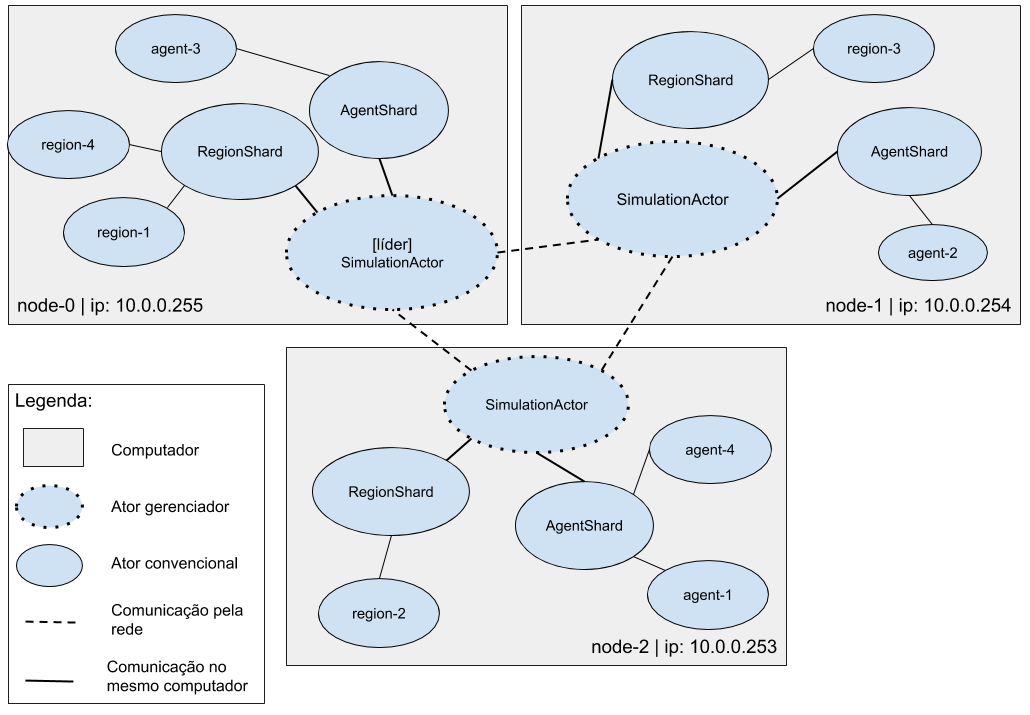
\includegraphics[scale=0.45]{imagens/d-optimas-new.png}
     \fonte{O próprio autor}
     \label{fig:d_optimas_new}
 \end{figure}
 
 A \autoref{fig:d_optimas_new} ilustra a nova organização proposta da arquitetura. Cada ator é representado por uma elipse, os responsáveis por gerenciar a simulação tem a borda pontilhada, e os agentes e regiões, por sua vez, têm as bordas contínuas. As linhas contínuas indicam que os atores se comunicam no mesmo nó, e as linhas tracejadas indicam que os atores se comunicam através da rede. A imagem exemplifica um \textit{cluster} composto por 3 computadores. 
 
 A arquitetura é agora composta de um único ator supervisor por processo, chamado \textbf{SimulationActor}, responsável por gerenciar tanto as regiões quanto os agentes. Quando um nó começa a executar, este é o primeiro ator a ser criado, e há um único para cada processo em execução. O \textbf{SimulationActor} subscreve nos eventos do \textit{cluster} de novo membro (\textbf{MemberUp}), saída de um membro (\textbf{MemberDown}) e de mudança de líder (\textbf{LeaderChanged}), de modo que ele recebe uma mensagem quando qualquer um desses eventos acontece. Quando um segundo nó começa a executar, ambos recebem uma mensagem de que há um novo membro na simulação. Neste ponto, a biblioteca \textit{akka-cluster} elege um líder. Doravante, sempre que o \textbf{SimulationActor} for mencionado, este deve ser associado imediatamente com o líder da simulação, e caso seja necessário falar de um outro ator do mesmo tipo em um nó qualquer, essa distinção será feita. 
  
 O líder tem um papel importante ao longo da execução da simulação. Dentro da especificação da biblioteca \textit{akka-cluster}, ele é o responsável por tarefas administrativas relacionadas ao \textit{cluster}, como por exemplo permitir a entrada de novos membros ou remover um nó que está em estado inacessível. No caso da simulação do D-Optimas, o \textbf{SimulationActor} também é o responsável por iniciar e finalizar a simulação, criar e destruir regiões e manter os agentes atualizados sobre o estado do espaço de busca. Ele também mantém dados estatísticos das regiões, que serão detalhados na seção a seguir. 
 
Ao longo do texto pode parecer que o líder tem um papel crítico na execução da simulação, e que isso pode caracterizar algum tipo de gargalo, ponto único de falha ou controle central. Entretanto, o líder exerce fundamentalmente um papel de coordenador, podendo inclusive ser mudado ao longo da simulação. Executar algumas das tarefas no líder é uma mera questão de escolha, por ser uma maneira mais simples de implementar um algoritmo num ambiente distribuído, sem a adoção um controle central. Isso tão pouco caracteriza um controle central, pois caso um líder fique inoperante, outro nó assume a liderança quase que imediatamente, sem causar prejuízo ou interrupção da simulação. Este comportamento já é um importante passo dado na direção de promover um sistema resiliência a falhas, desde  que seja possível restaurar os agentes/regiões que estavam subordinados ao nó falho. 
 
 Como foi dito, para cada processo criado há um único ator do tipo \textbf{SimulationActor}, que supervisona outros dois atores, o \textit{\textbf{agentShard}} e o \textit{\textbf{regionShard}}. Um ator do tipo \textit{\textbf{Shard}}, disponibilizado na biblioteca \textit{akka-sharding}, um sub-pacote do \textit{akka-cluster}, é o responsável por oferecer transparência de localidade dentro de um \textit{cluster}. Isso permite que os agentes e regiões  troquem mensagens pelo seu endereço lógico, em geral, o nome do ator, em detrimento de seu endereço completo. Caso o \textit{agent-1} queira enviar uma mensagem para a \textit{region-4}, essa mensagem é enviada juntamente com o identificador do destinatário à \textit{shard} mais próxima, que sabe como encaminhar a mensagem ao destinatário. 
 
 Além da transparência de localidade, a biblioteca \textit{akka-sharding} oferece persistência aos atores, utilizando um banco de dados interno e distribuído, baseado em CRDTs (\textit{Conflict-free Replicated Data Types})\cite{shapiro2011}. Isso permite que atores migrem de um \textit{Shard} para outro, caso o primeiro nó esteja mais sobrecarregado que o segundo. A utilização do banco de dados distribuído também permite que, caso um nó falhe, os agentes e regiões sejam restaurados em outro nó, no último estado registrado no banco. Portanto, a arquitetura possui neste ponto algum nível de resiliência a falhas, e também o balanceamento de carga entre os nós. 
 

 
\section{Da dinâmica do espaço de busca e interações entre regiões e o SimulationActor}
\label{sec:dinamica}
% procedimento de inserir uma nova solução
Uma vez construído o sistema, com os agentes e regiões comunicando entre si por meio dos \textit{shards} e conectados ao líder da simulação com auxílio do \textit{akka-cluster}, o próximo passo é entender o comportamento das regiões no sistema. São quatro os algoritmos associados à essa dinâmica: a criação de novas regiões, a inserção de uma solução em uma região, a fissão de uma região e a fusão de duas regiões. 

O primeiro cenário que será abordado é quando um agente produz a primeira solução do sistema e quer enviá-la à uma região. Como o agente tem um conhecimento parcial do mundo, ele sempre envia essa solução para o ator gerenciador da simulação. Sendo as regiões conjuntos não-vazios de soluções, a simulação não possui nenhuma região até que a primeira solução seja criada. O \textit{SimulationActor} é o responsável por criar esta nova região que abrigará aquela solução. Para criar uma região, o \textit{SimulationActor} envia uma mensagem do tipo \textbf{CreateRegion} ao \textbf{RegionShard} subordinado a ele. Internamente, o \textit{akka-cluster} decide em qual nó da simulação essa região vai ser criada, não sendo necessariamente no mesmo nó. Essa decisão será tomada com base no balanceamento das \textbf{Shards}. Uma nova região é criada para cada nova solução recebida até que o sistema atinja o número mínimo de regiões em toda a simulação, que é um parâmetro de configuração do sistema fornecido pelo usuário no arquivo de configuração da simulação. Quando atingido esse limite mínimo, o sistema passa a escolher aleatoriamente a região que receberá a próxima solução.

Esse procedimento aleatório se repetirá até que as regiões tenham pelo menos duas soluções. A partir desse momento, o \textbf{SimulationActor} passa a manter alguns dados relativos às regiões, que são: o valor médio, a variância e o coeficiente de variação das funções objetivo de todas as soluções, bem como o número de soluções para cada região. As fórmulas para o cálculo de cada um desses parâmetros estão descritas na \autoref{tab:formulas}. Ele também agrega os dados de cada região para calcular a estatística global do sistema, que compreende a média, desvio padrão e o coeficiente de variação dos valores de função objetivo de todas as soluções existentes, aqui denotados por $\bar{x}_g$, $s_g$ e $CV_g$, respectivamente.

No momento em que cada região tem ao menos duas soluções e o $CV$ de todas as regiões é diferente de zero, para cada nova solução recebida, o \textbf{SimulationActor} sorteia a região que receberá a próxima solução baseado no coeficiente de varição das regiões: regiões com maior $CV$ tem menor probabilidade de receber soluções, enquanto regiões com menor $CV$ tem chances maiores chances de serem escolhidas. Quando uma região recebe uma solução, ela envia uma mensagem do tipo \textbf{UpdateRegionSummary} para o líder, que atualiza a estatística da região, recalcula a estatística global e envia-a para todas as regiões, através de uma mensagem \textbf{UpdateGlobalSummary} contendo os valores de $\bar{x}_g$, $s_g$ e $CV_g$. 

Sempre que o \textbf{SimulationActor} recebe uma nova solução ele também incrementa um contador, que é considerado o tempo discreto da simulação. Esse tempo é propagado para todos os elementos do \textbf{cluster}, incluíndo os agentes e regiões, utilizando a estratégia de \textit{pig backing} sobre a mensagem de \textbf{UpdateGlobalSummary}. Apesar de funcionar como um relógio lógico global  \cite[p. 244]{tanenbaum}, o tempo discreto não tem o objetivo de criar qualquer mecanismo de sincronização entre os membros da simulação. As mensagens que transmitem soluções são marcadas com esse tempo que é utilizado posteriormente para forçar uma ordenação parcial entre os eventos, facilitando a extração e analise de dados. 

\begin{table}[]
    \centering
    \renewcommand{\arraystretch}{1.5} % Default value: 1
    \caption{Fórmulas utilizadas para calcular os parâmetros de uma região $r$ com $n$ soluções $x_i$, e uma função objetivo é $f(\cdot)$ }
    \label{tab:formulas}
    \begin{tabular}{cc}
        \toprule
         \textbf{Parâmetro} & \textbf{Fórmula} \\
         \midrule
         \\
         Média ($\bar{x}$) & \( \displaystyle \sum_{i = 1}^{i \leq n} f(x_i) \) \\ \\
         Variância ($s^2$) & \( \displaystyle \frac{1}{n - 1} \sum_{i = 1}^{i \leq n} (\bar{x} - f(x_i))^2 \) \\ \\
         Coeficiente de variação ($CV$) & \( \displaystyle \frac{s}{\bar{x}} \) \\ \\
         \bottomrule
    \end{tabular}
\end{table}

No que diz respeito à estratégia de escolha das regiões baseada no $CV$, há outras diferentes formas de se fazer essa escolha, \textit{e.g.} sortear aleatoriamente uma região para receber uma solução. Entretanto, o presente trabalho não pretende avaliar o mérito de uma estratégia, ou comparar esta com qualquer outra. O sorteio probabilístico foi escolhido por ser um algoritmo simples, mas não trivial. O algoritmo proposto não oferece nenhuma garantia sobre como a adição de uma nova solução a uma região particular afetará a distribuição dos valores de função objetivo, podendo fazer essa região tanto se tornar mais especializada, com o $CV$ menor, menos especializada, aumentando  o $CV$. A única premissa do procedimento adotado é que regiões muito especializadas tem mais chances de crescerem em quantidade de soluções. 

% dinâmica interna
As regiões, apesar de não escolherem quais soluções receberão, tem autonomia para se particionar ou se fundir, sendo assim entidades ativas do sistema. Como atores da plataforma \textit{akka} são entidades reativas que somente respondem a mensagens, que podem ter sido enviadas por um outro ator ou pelo próprio receptor, foi utilizado um artifício já proposto por \citeonline{pacheco}. As regiões recebem uma mensagem chamada \textbf{InternalBehaviour}, que é enviada periodicamente pela própria região. Ao receber essa mensagem, a receptora deve escolher, com uma probabilidade de 50\% entre se separar em três outras regiões ou se fundir com uma outra região.

% split das regiões 

Caso uma região região $r$ escolha fazer a fissão, ela deve se certificar de que  duas condições sejam satisfeitas. A primeira delas é que a região possua um número mínimo de soluções, cujo valor é dado pelo usuário no início da simulação. Esse parâmetro existe para evitar que uma região se particione prematuramente. A segunda condição é que o coeficiente de variação dos valores de função objetivo da região $r$ seja maior que o coeficiente de todas as soluções do sistema, \textit{i.e.},  $CV_r > CV_g$. 

Caso essas duas condições sejam satisfeitas a região $r$ se particionará em outras 3 regiões, a saber, as soluções cujo valor de função objetivo estão abaixo de $\bar{x}_{r} - s_{r}$ (cauda inferior), as soluções que estão acima de $\bar{x}_{r} + s_{r}$ (cauda superior) e as soluções que estão entre $\bar{x}_{r} - s_{r}$ e  $\bar{x}_{r} + s_{r}$, onde $\bar{x}_r$ e $s_r$ são a média e o desvio padrão dos valores de função objetivo das soluções que pertencem a região $r$, respectivamente. 

Ao se particionar, a região envia ao \textit{SimulationActor} uma mensagem do tipo \textit{RegionSplit} contendo dois conjuntos de soluções, as da cauda superior e inferior da distribuição. As soluções do centro da distribuição ficam com a região $r$. Ao receber uma mensagem do tipo, \textbf{SimulationActor} verifica se o número máximo de regiões permitidas no sistema não foi atingido, cria as novas regiões com a soluções recebidas. Caso o número máximo já tenha sido atingido, o sistema redistribui aleatoriamente as soluções entre as regiões já existentes. Esse parâmetro do número máximo de regiões também é fornecido no arquivo de configuração do sistema e é necessário para evitar o crescimento exacerbado do número de regiões, levando o sistema a consumir memória de maneira desordenada. 

% procedimento de merge
Caso a região $r_1$ decida por tentar fazer a fusão, ela enviará uma mensagem do tipo \textbf{MergeRequest} para todas as regiões contendo os seus parâmetros estatísticos. Ao receber uma mensagem desse tipo, uma outra região $r_2$ verifica se a união dos dois conjuntos de solução produzira uma nova região $r_3$ cujo $CV_{r_3}$ é menor do que o parâmetro $CV_{r_2}$. Caso essa condição seja satisfeita, a região $r_2$ responde à região $r_1$ com uma mensagem do tipo \textbf{MergeResponse}. Recebendo a primeira mensagem desse tipo, a região $r_1$ imediatamente envia uma mensagem do tipo \textbf{MergeResult} contendo a sua lista de soluções, e se destrói. Outras regiões que tenham respondido à solicitação de $r_1$ terão suas respostas ignoradas, não causando nenhum prejuízo ao sistema.

\begin{quadro}[ht!]
    \centering
    \caption{Mensagens trocadas na arquitetura D-Optimas}
    \label{tab:mensagens}
    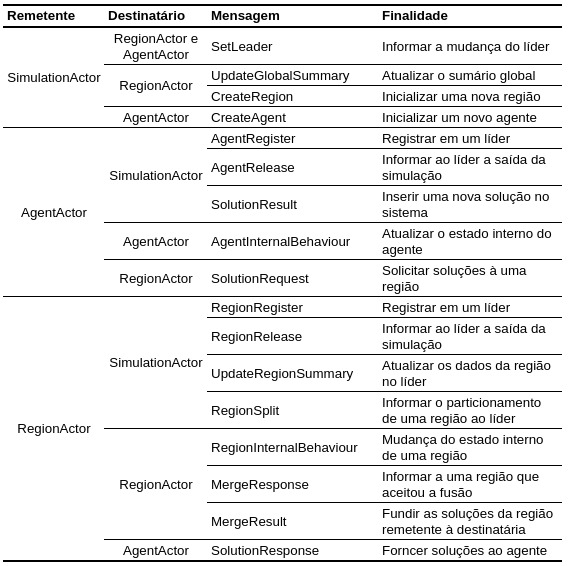
\includegraphics[scale=0.75]{imagens/tabela.jpeg}
    \begin{comment}
\begin{tabular}{lr{2}r{2.5}r{2}}\toprule
\textbf{Remetente} &\textbf{Destinatário} &\textbf{Mensagem} &\textbf{Finalidade} \\\midrule
\multirow{4}{*}{SimulationActor} &RegionActor e AgentActor &SetLeader &Informar a mudança do líder \\
&\multirow{2}{*}{RegionActor} &UpdateGlobalSummary &Atualizar o sumário global \\
& &CreateRegion &Inicializar uma nova região \\
&AgentActor &CreateAgent &Inicializar um novo agente \\
\multirow{5}{*}{AgentActor} &\multirow{3}{*}{SimulationActor} &AgentRegister &Registrar em um líder \\
& &AgentRelease &Informar ao líder a saída da simulação \\
& &SolutionResult &Inserir uma nova solução no sistema \\
&AgentActor &AgentInternalBehaviour &Atualizar o estado interno do agente \\
&RegionActor &SolutionRequest &Solicitar soluções à uma região \\
\multirow{8}{*}{RegionActor} &\multirow{4}{*}{SimulationActor} &RegionRegister &Registrar em um líder \\
& &RegionRelease &Informar ao líder a saída da simulação \\
& &UpdateRegionSummary &Atualizar os dados da região no líder \\
& &RegionSplit &Informar o particionamento de uma região ao líder \\
&\multirow{3}{*}{RegionActor} &RegionInternalBehaviour &Mudança do estado interno de uma região \\
& &MergeResponse &Informar a uma região que aceitou a fusão \\
& &MergeResult &Fundir as soluções da região remetente à destinatária \\
&AgentActor &SolutionResponse &Forncer soluções ao agente \\
\bottomrule
\end{tabular}
\end{comment}
\end{quadro}

O \autoref{tab:mensagens} apresenta um resumo de mensagens do sistema, bem como a finalidade de cada mensagem. 

\section{Do mecanismo de memória Q-learning}

% o que é o q-learning
% qual o modelo básico de atualização da tabela q-learning
% como esse modelo foi adaptado para funcionar com valores de função objetivo 
% como o agente utiliza a memória

\section{Adição de novos algoritmos populacionais}
\label{sec:algoritmos}

Um princípio fundamental na construção da arquitetura D-Optimas é de que a diversidade de estratégias de busca pode, não só levar a arquitetura a encontrar soluções de maior qualidade, quanto melhorar o desempenho geral em diferentes tipos de problema. A cada nova versão da arquitetura, alguns novos algoritmos foram adicionados, em especial na versão de \citeonline{denise2014}, que adicionou vários algoritmos construtores e de busca local. Entretanto, pouco esforço foi empreendido na adição de algoritmos evolutivos ou populacionais, técnica consolidada para solução de problemas complexos, dos quais a única premissa necessária é a de localidade fraca \cite{gaspar2012}.

Neste sentido, fez-se um esforço no presente trabalho de trazer ao menos mais duas técnicas populacionais/evolutivas à arquitetura, de modo que pudessem ser conduzidos experimentos para avaliar o efeito da diversidade de estratégias de busca, algo que não foi testado em trabalhos passados. Os algoritmos inseridos foram o \textit{Differential Evolution} (\textbf{DE}) \cite{storn1997} e o \textit{Particle Swarm Optimization} (\textbf{PSO}) \cite{eberhart1995, eberhart1998}. O algoritmo DE foi escolhido principalmente pela sua simplicidade, uma vez que possui poucos parâmetros de configuração. Por sua vez, o PSO foi escolhido por ser um dos algoritmos de otimização mais citados na literatura, tendo sido aplicado com sucesso em diversos problemas de otimização contínua \cite{bonyadi2017}. 

Ambos os algoritmos foram implementados somente para o problema de otimização irrestrita de função real, para o qual esses algoritmos foram inicialmente propostos. Entretanto, ambos foram implementados usando o arcabouço de generalização proposto por \citeonline{denise2014}, o que torna fácil a extensão deles para problemas de natureza combinatória, bastando implementar os modificadores adequados. Os parágrafos a seguir apresentam os pseudocódigos das estratégias de busca e como eles foram implementados e adaptados para a arquitetura D-Optimas, utilizando os mecanismos de generalização. 

\begin{figure}[ht!]
    \centering
    \caption{Diagrama das estruturas abstratas proposta por \citeonline{denise2014} e como elas foram  utilizadas na implementação dos algoritmos já existentes na arquitetura. As estruturas Problema, Solução e Analise de Solução são comuns a todas implementação de metaheurística. As siglas RMS e RMCS significam, respectivamente, as estruturas de Realiza Modificação de Solução e Realiza Modificação de Conjunto de Solução. São as principais estruturas utilizadas no presente trabalho para implementação dos algoritmos escolhidos. }
    \label{fig:denise_abstract_structures}
    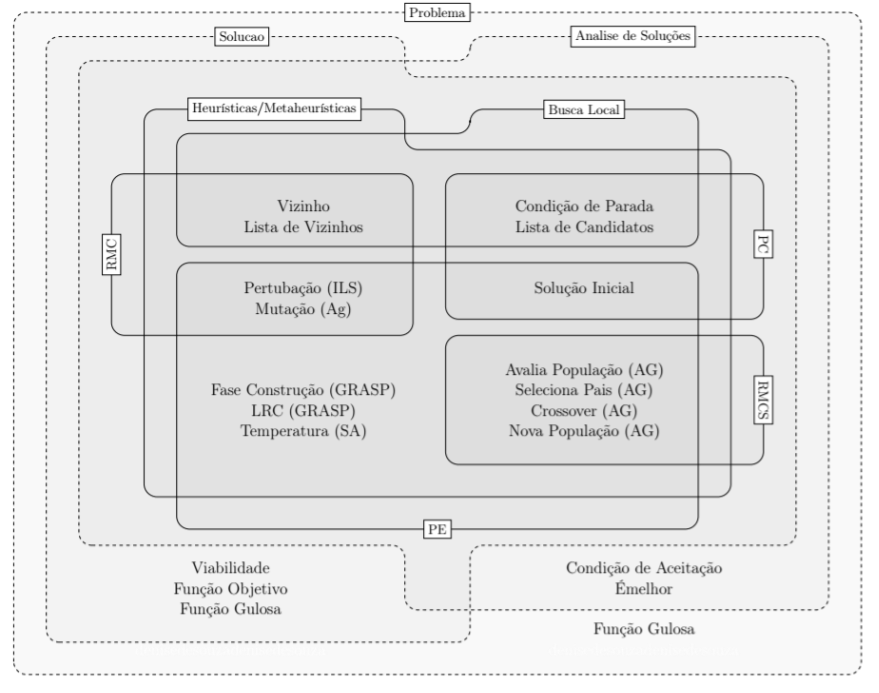
\includegraphics[scale=0.5]{imagens/denise-abstract-structures.png}
\end{figure}

Como já abordado no capítulo anterior \citeonline{denise2014} criou um conjunto de classes abstratas para implementar algoritmos de otimização que sejam independentes dos dados do problema, bem como da representação das soluções. A \autoref{fig:denise_abstract_structures} apresenta essas estruturas abstratas e suas relações com os algoritmos já implementados na arquitetura. Um exemplo é o \textit{Genetic Algorithm} (\textbf{GA}), que utiliza a estrutura de Modificador de Conjunto de Soluções (RMCS) para encapsular a avaliação da população, a seleção dos pais, o cruzamento e a seleção da nova população. 

Portanto, para incluir um novo algoritmo utilizando essas ferramentas foi necessário estudá-las e identificar em cada algoritmo quais os pontos em comum que poderiam depender de um problema específico e encapsulá-los na estrutura apropriada. Deste modo, serão apresentados à seguir os pseudocódigos dos dois algoritmos selecionados, do \textbf{DE} e do \textbf{PSO}, a ideia central da metaheurística e quais trechos foram encapsulados em estruturas abstratas.

A primeira metaheurística abordada será o \textbf{DE}, cujo pseudocódigo é apresentado no \autoref{algo:de}. Essencialmente o algoritmo aplica uma regra simples de seleção e mutação em cada indivíduo da população, sucessivamente, até que uma condição de parada seja atingida. Na implementação original uma população inicial é gerada aleatoriamente. Esse passo foi substituído, evidentemente, pelo comportamento padrão dos agentes na arquitetura que é solicitar um conjunto de soluções às regiões (linha 1). A condição de parada (linha 2) segue o padrão das outras implementações na arquitetura D-Optimas, e é informada pelo usuário no arquivo de configuração da simulação. Há atualmente algumas condições de parada implementadas na arquitetura que estendem a classe abstrata \textbf{StopCondition}. As implementações possíveis são a parada por número máximo de iterações, número máximo de iterações sem melhora, valor da melhor avaliação de função objetivo, tempo máximo de execução ou uma combinação qualquer das condições anteriores. 

A classe \textbf{DE} é composta de dois modificadores, o primeiro responsável por sortear os indivíduos para o cruzamento, o que corresponde a linha 4 do pseudocódigo, e o segundo corresponde a regra de mutação. Como esse modificador recebe uma lista de soluções, que é a população atual, e retorna uma lista contendo três soluções, este modificador é do tipo \textbf{ModifiesSolutionCollection}. O componente recebeu o nome de \textbf{DERandSelection}. 

\begin{algorithm}[H]
\caption{Evolução Diferencial}
\label{algo:de}
\begin{algorithmic}[1]
    \State{$t \gets 1$}
    \State \text{Recebe uma população inicial $X_t$ de tamanho $n$ e dimensão $D$} 
    \While{Condição de parada não for atingida} 
        \For{$i \gets 1$ até $n$} 
            \State{Sorteie $r_1, r_2, r_3 \in {1,\dots,n}$} 
            \State{Sorteie $i_{rand} \in {1, \dots, n}$}
            \For{$j \gets 1$ até $D$}
                \If{$rand(0,1) \leq CR \lor i = i_{rand}$}
                    \State{$u_{t,i,j} = x_{t,i,r_3} + F * (x_{t,i, r_1} - x_{t,i,r_2})$}
                \Else
                    \State{$u_{t,i,j} = x_{t,i,j}$}
                \EndIf
            \EndFor
        \EndFor
        
        \For{$i \gets 1$ até $n$}
            \If{$f(u_{t,i}) < f(x_{t,i})$}
                \State{$x_{t+1,i} \gets u_{t,i}$}
            \Else
                \State{$x_{t+1,i} \gets x_{t,i}$}
            \EndIf
        \EndFor
        \State{$t \gets t + 1$}
    \EndWhile
\end{algorithmic}
\end{algorithm}

As linhas 6 à 12 do \textbf{DE} foram encapsuladas em o segundo modificador de conjunto de soluções, que recebe uma lista contendo quatro soluções e aplica a regra de mutação descrita no algoritmo. Esse modificador foi implementado na classe  \textbf{DEMutationMSC}. 

Há algumas variações para as regras de seleção e mutação do algoritmo \textbf{DE}, que podem ser expressas de uma maneira sintética, de acordo com \citeonline{gaspar2012}. A variação implementada foi \texttt{DE/rand/1/bin}. Entretanto, outras variações podem ser facilmente implementadas sem grandes modificações da classe \textbf{DE}, simplesmente provendo novos modificadores.

A implementação do \textbf{DE} apresenta muito menos desafios do que o algoritmo \textbf{PSO}, cujo pseudocódigo é apresentado no \autoref{algo:pso}. O primeiro problema é a manutenção de duas populações, um vetor de posições que são as soluções do problema de otimização, e uma segunda população que são os vetores de velocidades associados às posições. O comportamento básico do algoritmo é atualizar, a cada iteração, o vetor de velocidade de cada partícula e logo em seguida atualizar a posição até que uma condição de parada seja atingida. Novamente, foi utilizada a estrutura abstrata de \textbf{StopCondition}, cuja implementação concreta é informada no arquivo de configuração da simulação. Para isso, o algoritmo além de receber as soluções iniciais das regiões (linha 1), gera um conjunto de soluções do mesmo tamanho que o primeiro conjunto e inicializa todas aleatoriamente chamando o método \textit{generateInitialSolution()}, definido na classe abstrata \textbf{Solution}. Novamente, foi utilizada a condição de parada genérica \textbf{StopCondition}, cujo tipo concreto é informado no arquivo de configuração da simulação. 

\begin{algorithm}[H]
\caption{Otimização por Enxame de Partículas}
\label{algo:pso}
\begin{algorithmic}[1]
    \State \text{Recebe uma população inicial $X$ de tamanho $n$ e dimensão $D$} 
    \State \text{Gere um conjunto de soluções aleatórias $V$ de tamanho $n$ e dimensão $D$}
    
    \While{Condição de parada não for atingida} 
        \For {$i \gets 1$ até $n$}
            \If{$f(x_i) < f(pb_i)$}
                \State $pb_i \gets x_i$ 
            \EndIf
            
            \If{$f(x_i) < f(gb)$}
                \State $gb \gets x_i$
            \EndIf
        \EndFor
    
        \For {$i \gets 1$ até $n$}
            \For{$d \gets 1$ até $D$}
                \State{$v_{i,d} \gets v_{i,d} + C_1 * rand(0, 1) * (pb_{i,d} - x_{i,d}) + C_2 * rand(0, 1) * (gb_d - x_{i,d}) $}
                \State{$x_{i,d} \gets x_{i,d} + v_{i,d}$}
            \EndFor
        \EndFor
    \EndWhile
\end{algorithmic}
\end{algorithm}

O algoritmo mantém uma terceira lista de soluções que armazena a melhor posição de cada indivíduo do enxame ao longo da execução do algoritmo, que corresponde no pseudocódigo à variável $pb_i$. Além desta memória, ele também mantém melhor partícula ao longo da execução, que corresponde à variável $gb$. A cada iteração essas variáveis são atualizadas, e para fazer a comparação, utilizamos a classe abstrata  \textbf{SolutionAnalizer}, que fornece métodos para efetuar a comparação entre duas soluções. Essa classe deve ser estendida e o seu tipo concreto também é informado no arquivo de configuração. 

Os passo de alteração dos vetores velocidade e posição foram implementados em dois modificadores de coleção diferentes. Para modificar as velocidades, é necessário passar um vetor de tamanho $2*n + 1$, contendo nas $n$ primeiras posições os vetores de velocidade, nas $n$ posições seguintes o vetor $pb$ e na última posição da lista a melhor solução até a t-ésima iteração $gb$. Esse modificador foi nomeado \textbf{PSOVelocityUpdateMSC} e corresponde a linha 14 do \autoref{algo:pso}. Por fim, o modificador \textbf{PSOPositionUpdateMSC} recebe uma lista de tamanho $2n$ contendo nas $n$ primeiras posições o vetor $X$ e nas $n$ posições seguintes o vetor V  atualiza a lista de posições, encapsulando a linha 15 do pseudocódigo.

\section{Considerações finais}
O presente capitulo se dedicou a apresentar as alterações feitas na arquitetura D-Optimas, proposta inicialmente por \citeonline{pacheco}. Essas alterações tiveram o principal objetivo de melhorar aspectos teóricos e evoluir a arquitetura, por exemplo, conferindo resiliência à simulação, do ponto de vista de sistemas distribuídos e dando uma definição precisa para o comportamento das regiões. Foram adicionadas também mais estratégias de busca, para cumprir o propósito da D-Optimas, como um sistema multi-agente, onde há diversidade de estratégias.

O capitulo seguinte apresentará alguns experimentos preliminares para avaliar as mudanças que foram feitas até o momento, principalmente no que diz respeito ao desempenho computacional e a escalabilidade da arquitetura.
 
 % -----------------------------------------------------------------------------
%   Arquivo: ./02-elementos-textuais/resultadosEsperados.tex
% -----------------------------------------------------------------------------


\chapter{Avaliação da escalabilidade}
\label{chap:exp_preliminares}

Apresentadas as correções e aprimoramentos feitos na arquitetura D-Optimas, é necessário avaliar os impactos no seu funcionamento e comportamento. Neste capítulo será apresentada uma  bateria de experimentos, com o objetivo de avaliar a escalabilidade da nova implementação baseada em \textit{akka-cluster}.

A \autoref{sec:desempenho} descreve o experimento para avaliar o impacto do aumento da quantidade de nós do \textit{cluster} na execução da simulação, principalmente na latência entre as mensagens trocadas e a taxa de produção de soluções dos agentes. A \autoref{sec:resultado} apresenta os resultados obtidos e a análise estatística para cada tipo de mensagem analisada. Espera-se que, mantendo o número de agentes e o limite de regiões, mas aumentando o número de nós, a carga seja melhor distribuída entre os nós, e que o tempo médio entre um envio de uma mensagem por um ator e o seu respectivo processamento em outro ator diminua. Por fim, a \autoref{sec:sintese} apresenta uma síntese dos resultados. 

\section{Avaliação de desempenho da arquitetura}
\label{sec:desempenho}

Esse experimento avaliou a média da latência das trocas de mensagens entre os agentes, regiões e atores supervisores da simulação. O número de nós do \textit{cluster} em que a arquitetura executou foi o único parâmetro que sofreu variação. 

Foram executadas 4 instâncias, nomeadas S3, S4, S5 e S6, utilizando de 3 a 6 nós. Para cada instância do experimento foram obtidas 14 réplicas da mesma configuração, que é exibida no \autoref{tab:expS}. Cada execução contou com 18 agentes, sendo 6 agentes construtores, 6 populacionais e 6 agentes de busca local. Os agentes construtores tiveram o tempo de vida limitado à 200 unidades pois as soluções por eles geradas servem somente como soluções iniciais.
Para este experimento os mecanismos de aprendizagem e memória dos agentes foram desabilitados, uma vez que a mudança na organização do sistema impacta fortemente no funcionamento desses componentes. 
Além destas configurações, ficou estabelecido o número limite de 100 regiões no sistema, o número mínimo de 30 soluções para uma região se particionar, e o tempo limite de 1000 unidades para que a simulação fosse interrompida.

O ambiente computacional utilizado foi o \textit{cluster} do Laboratório de Sistemas Inteligentes (LSI) do CEFET, composto de seis máquinas com processador Intel i7, 32GB de RAM e 2TB de HD cada. O sistema operacional utilizado foi o CentOS 6, e o SLURM como escalonador
de tarefas. A versão do JDK (\textit{Java Development Kit}) utilizada foi a 12.0.1.

\begin{table}
\caption{\label{tab:expS}Parâmetros das meta-heurísticas}
\centering

\begin{tabular}{lllc}
    \toprule
    \textbf{Nº de agentes}  & \textbf{Metaheurística}   & \textbf{Parâmetro}        & \textbf{Valor} \\
    \midrule
    \multirow{2}{*}{6}      & \multirow{2}{*}{GRASP}    & iterações                 & 100\\
                            &                           & iterações busca local     & 100\\
                            &                           & alpha                     & 0.5\\
    \midrule
    \multirow{2}{*}{3}      & \multirow{2}{*}{ILS}      & iterações                 & 500\\
                            &                           & nível de distúrbio        & 10\\
    \midrule
    \multirow{2}{*}{3}      & \multirow{2}{*}{ILS}      & iterações                 & 500\\
                            &                           & nível de distúrbio        & 7\\
    \midrule
    \multirow{4}{*}{3}      & \multirow{4}{*}{GA}       & iterações                 & 300\\
                            &                           & tamanho da população      & 20\\
                            &                           & taxa de mutação           & 0.2\\
                            &                           & taxa de cruzamento        & 0.7\\
    \midrule
    \multirow{4}{*}{3}      & \multirow{4}{*}{GA}       & iterações                 & 500\\
                            &                           & tamanho da população      & 30\\
                            &                           & taxa de mutação           & 0.1\\
                            &                           & taxa de cruzamento        & 0.8\\
    \bottomrule
\end{tabular}
\end{table}

Foram escolhidos quatro tipos de mensagem para serem analisadas. A primeira escolhida foi \textbf{UpdateGlobalSummary} que é frequentemente enviada pelo líder da simulação a todas as regiões e agentes sempre que alguma mudança acontece no sistema. A segunda mensagem, do tipo \textbf{UpdateRegionSummary}, é enviada por uma região sempre que recebe uma nova solução, ou uma fissão ou fusão acontece. A terceira mensagem analisada, do tipo \textbf{RegionSplit}, é enviada pelas regiões ao líder da simulação sempre que uma região se particiona, e por fim, a quarta mensagem mensagem, do tipo \textbf{SolutionResponse}, é enviada aos agentes pelas regiões em resposta a uma solicitação de soluções. Neste subconjunto de mensagens  estão presentes as principais e mais frequentes interações entre os agentes, regiões e o líder. Os dados extraídos foram tratados, removendo eventuais anomalias (latências negativas, por exemplo) e a média das latências para cada execução, para cada tipo de mensagem, e foram computadas a média das latências para cada execução e para cada tipo de mensagem. 

Antes de apresentar e discutir os resultados, é necessário fazer uma observação acerca do tratamento dos dados. Entre as execuções, cada mensagem pode ter sido trocada um número diferente de vezes e algumas delas podem não ter sido recebidas. Isso faz com que a média das latências da mensagem do tipo \textbf{UpdateGlobalSummary} em uma execução tenha sido calculada com um número diferente de observações em cada uma das 14 repetições para cada um dos 4 fatores. Esse particularidade dos dados, somada à estocasticidade inerente à arquitetura, pode levar os dados a não se comportarem bem, ainda que essa amostragem esteja congruente com a definição do teorema do limite central. Dito isso, as premissas da ANOVA são verificadas para cada tipo de mensagem, e quando atendidas, o teste paramétrico é escolhido. Todos os testes estatísticos foram realizados com um nível de confiança de 95\%.


\section{Resultados do experimento}
\label{sec:resultado}

\begin{figure}
    \centering
    \caption{\textit{Boxplot} das médias das latências da mensagem \textbf{UpdateGlobalSummary} para 14 execuções da arquitetura D-Optimas com duração de 1000 unidades de tempo discreto em 3, 4, 5 e 6 nós do \textit{cluster} }
    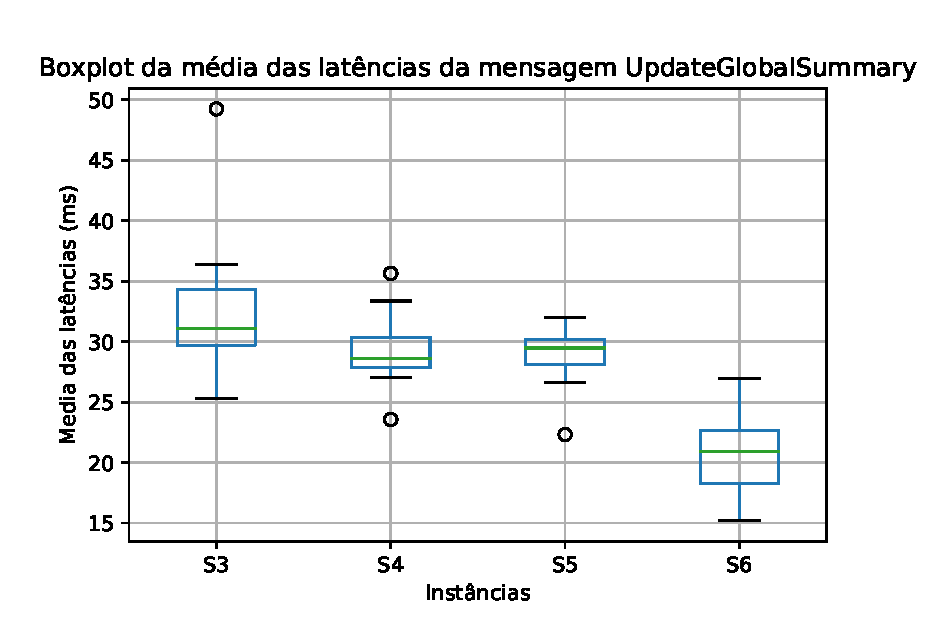
\includegraphics[scale=0.8]{imagens/update_global_summary.eps}
    \label{fig:update_global_summary}
\end{figure}

A \autoref{fig:update_global_summary} exibe o \textit{boxplot} das médias das latências das mensagens do tipo \textbf{UpdateGlobalSummary}. Visualmente é possível perceber que os dados estão bem comportados e há uma tendência de queda da latência a medida que o número de nós cresce. 

Para esse subconjunto dos dados, dois dos três pressupostos da ANOVA foram atendidos. O teste de Levene acusou um p-valor de $0.31538$, falhando em rejeitar a hipótese nula de que a variância dos resíduos é homogênea. Os resíduos são independentes mas não seguem uma distribuição normal, pelo teste de Shapiro-Wilk (p-valor de $0.000161$). Como a ANOVA é robusta a pequenas variações na normalidade, este teste foi escolhido. O p-valor obtido foi de $0$, indicando que há diferença em pelo menos uma das médias. 

A \autoref{tab:update_global_summary_tukey} exibe os resultados do teste de Tukey-HSD, para um nível de significância de $5\%$. O teste conclui que não há diferença entre as instâncias S3 e S4, e S4 e S5, onde há variação de apenas um nó no \textit{cluster}.

\begin{table}[ht!]
    \centering
    \caption{Comparações par-a-par (teste de Tukey-HSD) para as médias das latências de mensagens do tipo \textbf{UpdateGlobalSummary}}
    \begin{tabular}{cccc}
    \toprule
    \multicolumn{2}{c}{\textbf{Instâncias}} & \textbf{p-valor} & \textbf{Rejeita $H_0$?}\\
    \midrule
    S3   &  S4  & 0.0938 &  Não \\
    S3   &  S5  & 0.0451 &   Sim \\
    S3   &  S6  &  0.001 &   Sim \\
    S4   &  S5  &    0.9 &  Não \\
    S4   &  S6  &  0.001 &   Sim \\
    S5   &  S6  &  0.001 &   Sim \\
    \bottomrule
    \end{tabular}
    \label{tab:update_global_summary_tukey}
\end{table}

A segunda mensagem analisada foi a \textbf{UpdateRegionSummary}. A \autoref{fig:update_region_summary} exibe a distribuição das médias das latências para as quatro instâncias do experimento. Aparentemente há uma tendência de diminuição da variância a medida que a arquitetura escala. Os dados não atendem aos pressupostos de normalidade (com p-valor de $0.000121$) e homocedasticidade (p-valor de $0.004774$).  

Por isso, foi escolhido um teste não paramétrico de Kruskal-Wallis, para verificar se há diferença entre as instâncias. O teste produziu um p-valor de $0.002919$, que leva a rejeição da hipótese nula, indicando que há diferença em pelo menos uma das médias. 

\begin{figure}
    \centering    
    \caption{\textit{Boxplot} das médias das latências da mensagem \textbf{UpdateRegionSummary} para 14 execuções da arquitetura D-Optimas com duração de 1000 unidades de tempo discreto em 3, 4, 5 e 6 nós do \textit{cluster} }
    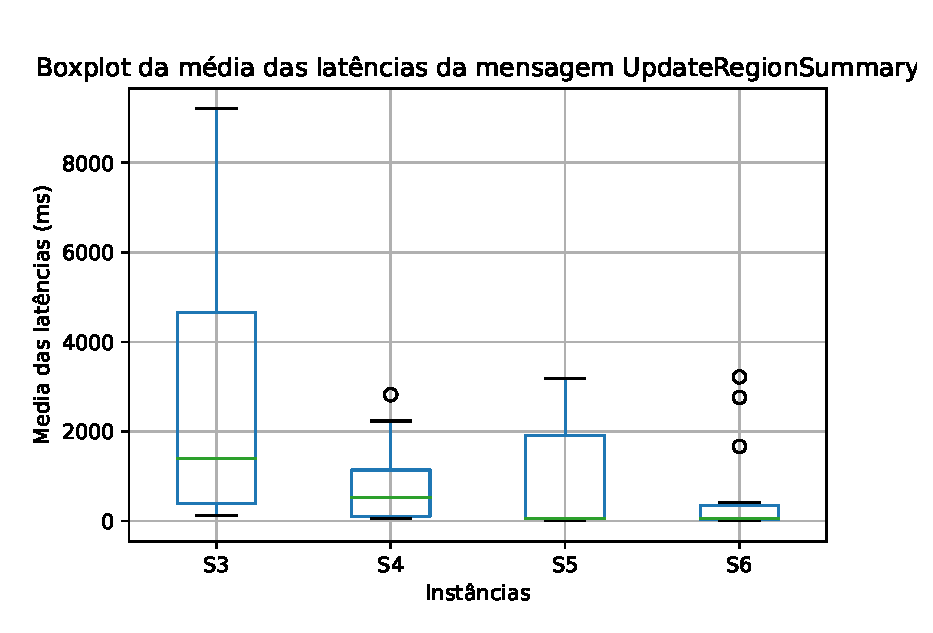
\includegraphics[scale=0.8]{imagens/update_region_summary.eps}
    \label{fig:update_region_summary}
\end{figure}

Para verificar em qual dos pares está a diferença, foi escolhido um teste \textit{post-hoc} não paramêtrico de Conover-Iman. Os p-valores obtidos pelo teste são apresentados na tabela \autoref{tab:update_region_summary}. É possível observar que há diferença sempre que se adiciona pelo menos dois nós na simulação.

\begin{table}[ht!]
    \centering
    \caption{Comparações par-a-par (Teste de Conover) para a média das latências de mensagens do tipo \textbf{UpdateRegionSummary}}
    \begin{tabular}{cccc}
    \toprule
    \multicolumn{2}{c}{\textbf{Instâncias}} & \textbf{p-valor} & \textbf{Rejeita $H_0$?}\\
    \midrule
     S3 &    S4 &  0.06021 &  Não  \\
     S3 &    S5 &  0.00378 &   Sim \\
     S3 &    S6 &  0.00017 &   Sim \\
     S4 &    S5 &  0.27176 &  Não  \\
     S4 &    S6 &  0.03905 &   Sim \\
     S5 &    S6 &  0.31895 &  Não  \\
     \bottomrule
    \end{tabular}
    \label{tab:update_region_summary}
\end{table}

A terceira mensagem  analisada foi a \textbf{RegionSplit}. O \textit{boxplot} das médias das latências para as quatro instâncias do experimento é apresentado na \autoref{fig:region_split}. Novamente é possível observar uma tendência de queda da latência a medida que novos nós são adicionados à simulação. Os pressupostos de normalidade e homocedasticidade não são atendidos, com p-valores de $0.000005$ e $0.002790$, respectivamente.  

\begin{figure}
    \centering
    \caption{\textit{Boxplot} das médias das latências da mensagem \textbf{RegionSplit} para 14 execuções da arquitetura D-Optimas com duração de 1000 unidades de tempo discreto em 3, 4, 5 e 6 nós do \textit{cluster} }
    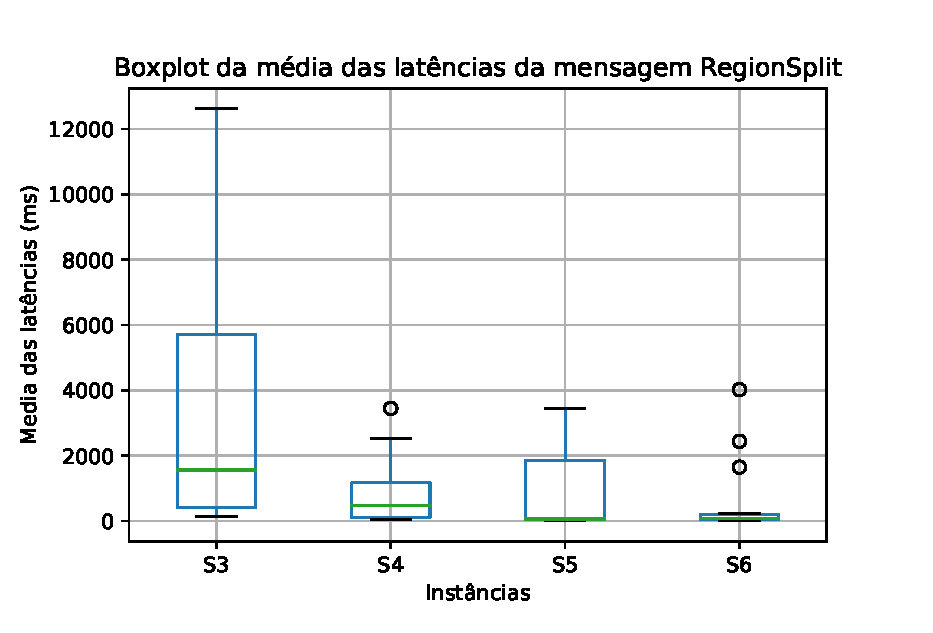
\includegraphics[scale=0.8]{imagens/region_split.eps}    \label{fig:region_split}
\end{figure}

O teste de Kruskal-Wallis produziu um p-valor de $0.0.002748$, o que indica uma diferença em pelo menos uma das médias. A \autoref{tab:region_split} apresenta os resultados do teste de Conover-Iman. O teste novamente indica que não é possível observar diferença na latência entre duas amostras com a variação de apenas um nó. Adicionando 2 nós, a diferença entre as médias da latência é significativa. 

\begin{table}[ht!]
    \centering
    \caption{Comparações par-a-par (Teste de Conover) para a média das latências de mensagens do tipo \textbf{RegionSplit}}
    \begin{tabular}{cccc}
    \toprule
    \multicolumn{2}{c}{\textbf{Instâncias}} & \textbf{p-valor} & \textbf{Rejeita $H_0$?}\\
    \midrule
       S3  &  S4  &  0.06021  &  Não \\
       S3  &  S5  &  0.00378  &   Sim \\
       S3  &  S6  &  0.00017  &   Sim \\
       S4  &  S5  &  0.27176  &  Não \\
       S4  &  S6  &  0.03905  &   Sim \\
       S5  &  S6  &  0.31895  &  Não \\
     \bottomrule
    \end{tabular}
    \label{tab:region_split}
\end{table}


Finalmente, a distribuição das médias das latências para as mensagens do tipo \textbf{SolutionResponse} são exibidas na \autoref{fig:solution_response}. Pela análise gráfica é possível dizer que há diferença entre a instância S3 e S4, S5 e S6. As observações são independentes e as variâncias são homogêneas (com p-valor de $0.060870$). 

\begin{figure}
    \centering    
    \caption{\textit{Boxplot} das médias das latências da mensagem \textbf{SolutionResponse} para 14 execuções da arquitetura D-Optimas com duração de 1000 unidades de tempo discreto em 3, 4, 5 e 6 nós do \textit{cluster} }
    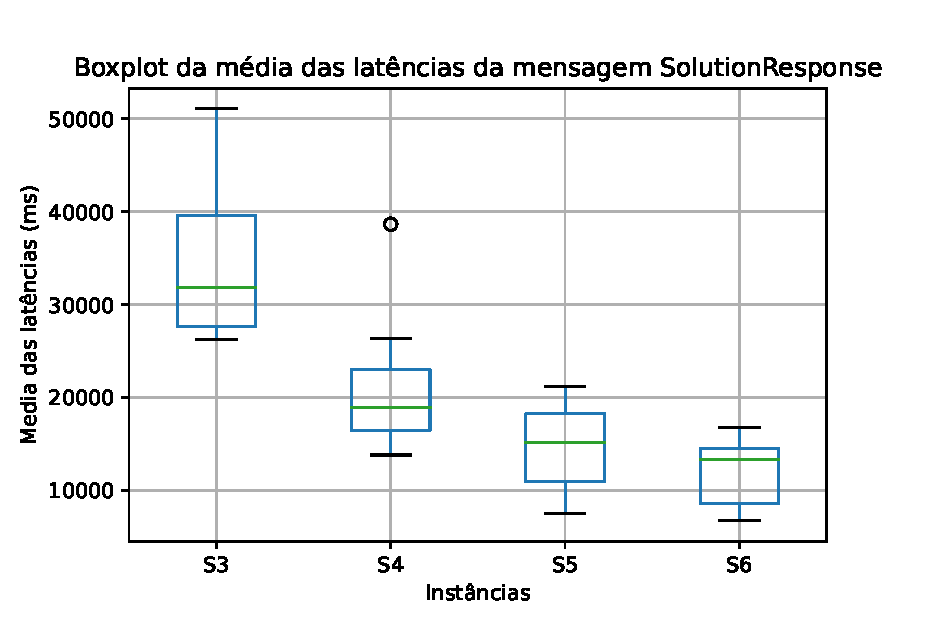
\includegraphics[scale=0.8]{imagens/solution_response.eps}
    \label{fig:solution_response}
\end{figure}

Há um pequeno desvio na normalidade, o que permite executar uma análise paramétrica. A ANOVA indica que há diferença entre as médias, com p-valor igual a $0$. A \autoref{tab:solution_response} indica que há diferença entre S4 e S6, além da diferença entre S3 que já era percebida na análise gráfica. 

\begin{table}[ht!]
    \centering
    \caption{Comparações par-a-par (Teste de Tukey-HSD) para a média das latências de mensagens do tipo \textbf{SolutionResponse}}
    \begin{tabular}{cccc}
    \toprule
    \multicolumn{2}{c}{\textbf{Instâncias}} & \textbf{p-valor} & \textbf{Rejeita $H_0$?}\\
    \midrule
    S3  &  S4 & 0.001   & Sim  \\
    S3  &  S5 & 0.001   & Sim  \\
    S3  &  S6 & 0.001   & Sim  \\
    S4  &  S5 &  0.0862 & Não \\
    S4  &  S6 &   0.004 & Sim  \\
    S5  &  S6 &  0.6325 & Não \\
     \bottomrule
    \end{tabular}
    \label{tab:solution_response}
\end{table}

\section{Síntese do resultado}
\label{sec:sintese}

% aumentar o tamanho do cluster sem aumentar a simulação fornece mais recursos, favorece o balanceamento de carga, e leva os atores a processarem mais rápido
De uma maneira geral, aumentar o tamanho do \textit{cluster}, mantendo a quantidade de agentes e o limite de regiões, significa oferecer mais recursos computacionais à arquitetura. A presença de mais núcleos de processamento, memória, largura de banda, favorece o balanceamento de carga. Ao distribuir melhor a carga entre os nós de processamento, é natural que o  escalonamento entre os atores, o tempo de espera por I/O e a paginação de memória diminuam, fazendo que cada execução do ator seja mais eficiente.

% os resultados mostram que há de fato uma tendência de queda quando o número de nós aumenta, e o número de entidades é mantido o mesmo
Dito isto, os resultados mostram que há de fato uma tendência de queda da latência média com o aumento do número de nós, em especial, sempre que mais de um nó é adicionado na simulação. Em outras palavras, os atores são mais rápidos em processar as mensagens que recebem. Essa tendência é um indício de que a arquitetura foi construída de maneira a aproveitar de maneira eficiente os recursos que estão disponíveis para ela. 

% mensagens que são recebidas pelo líder tem variância menos homogêneas, mas ainda assim parece haver uma tendência de queda a medida que o líder tem mais recursos computacionais
Entre os quatro tipos de mensagem analisadas neste experimento é possível observar que há uma diferença na ordem de grandeza e na variância comparando as mensagens recebidas pelo líder e as recebidas por outras entidades da simulação. É possível que este fenômeno seja reflexo de uma concentração de tarefas no líder. Mesmo que as tarefas não tenham uma complexidade computacional alta (a maioria delas possui complexidade assintótica da ordem $\mathcal{O}(n)$, onde $n$ é o número de agentes e regiões na simulação), pode haver uma demora em atender as mensagens que se acumulam rapidamente. Ainda assim, é possível observar que o líder se beneficia também do aumento de recursos computacionais, diminuindo a média da latência.

% para de fato verificar o potencial de escalabilidade da arquitetura, é necessário executar outros testes, variando outros fatores, por exemplo, o número máximo de regiões e o número de agentes em execução.
É preciso ressaltar que os resultados obtidos neste experimento não indicam uma escalabilidade da arquitetura sob qualquer condição. Os resultados são preliminares e dão bons indícios da resiliência da arquitetura como um sistema distribuído, mas para obter resultados mais robustos é necessário avaliar outros fatores, como por exemplo, o número máximo de regiões permitidas, o número de agentes em execução e o crescimento do conjunto de soluções produzido pela arquitetura. Além disso, é necessário avaliar o funcionamento da arquitetura num \textit{cluster} com dezenas ou centenas de nós. 

% esta avaliação é importante para verificar a eficiência do software, principalmente para oferecer a solução a um usuário final. De toda forma, este é um sistema de tempo discreto, uma latência baixa é desejável, mas não influência na qualidade das soluções. 
Avaliar o desempenho da D-Optimas é importante para certificar a correta implementação como um sistema distribuído, bem como a eficiência do \textit{software}, principalmente para oferecê-lo como uma ferramenta de trabalho para um usuário final, um tomador de decisão num processo de otimização. De todo modo, este é um sistema de tempo discreto, todas as meta-heurísticas são algoritmos discretos, que não dependem de resposta em tempo real. É claro que uma latência baixa é desejável, mas ela de fato não influencia na qualidade das soluções, somente no tempo de espera por soluções de boa qualidade.


\begin{comment}
\section{Avaliação do efeito da memória na qualidade das soluções produzidas}
% - O que esse experimento avaliou 
Este segundo experimento avaliou o efeito da adição da memória \textit{Q-learning} na qualidade das soluções produzidas pela arquitetura D-Optimas. 
% - Quais amostras foram coletadas
Para tanto, foram executadas duas configurações da arquitetura. A primeira configuração com a memória desabilitada, doravante denominada \textbf{NQ}, que servirá como \textit{baseline}. O segundo nível do experimento, de sigla \textb{Q}, corresponde à memória Q-learning habilitada em todos os agentes populacionais e buscas locais, com uma taxa de utilização da memória de 80\%.

% - Qual foi a configuração deste experimento
Para cada nível do experimento foram coletadas 19 amostras do melhor valor da função objetivo ao longo do tempo. Cada execução contou com 18 agentes, sendo 6 agentes construtores, 6 populacionais e 6 agentes de busca local. Os agentes construtores tiveram o tempo de vida limitado à 200 unidades pois as soluções por eles geradas servem somente como soluções iniciais. Os parâmetros de configuração de cada agente estão descritos na \autoref{tab:expQConfig}.
% - Quais os dados foram colhidos das amostras
Foram coletados os 19 melhores valores da função objetivo encontrados ao final de cada execução.  
% - Quais as ressalvas eu devo fazer a esse experimento

\begin{table}[]
    \centering
    \begin{tabular}{ccc}
         \textbf{Metaheurística}&\textbf{Parâmetro} & \textbf{Valor}  \\
         \multirow{3}{*}{GRASP}     & iterações             & 500   \\
                                    & iterações busca local & 100   \\
                                    & alpha                 & 0.5   \\
         \midrule
         \multirow{2}{*}{ILS}       & iterações             & 500   \\
                                    & distúrbio             & 7     \\
         \midrule
         \multirow{4}{*}{GA}        & iterações             & 500   \\
                                    & tamanho da população  & 30    \\
                                    & taxa mutação          & 0.2   \\
                                    & taxa de cruzamento    & 0.5   \\
         
    \end{tabular}
    \caption{Configuração dos agentes para o experimento que avaliou o efeito da memória \textit{Q-learning}}
    \label{tab:expQConfig}
\end{table}

\subsection{Resultado do experimento}


\subsection{Síntese do resultado}

\section{Considerações finais}

\end{comment}

 
 \chapter{Avaliação do efeito da diversidade na qualidade das soluções produzidas}
\label{chap:exp_diversidade}
\epigraph{Rir, antes da hora, engasga}{Riobaldo, em o \textit{Grande Sertão Veredas}}

Uma vez avaliada a capacidade de escalar horizontalmente, o atual capítulo descreverá os experimentos realizados para avaliar o efeito da diversidade de agentes na qualidade das soluções produzidas pela arquitetura.

Esta bateria de experimentos foi executada em máquinas virtuais no \textit{Google Cloud Platform}\footnote{https://cloud.google.com/compute/docs/machine-types}, em instâncias do tipo e2-standard-4 com 4 vCPUs e 8Gb de memória RAM. Nestes experimentos, a arquitetura executou como um único nó, conectada a dois nós do banco de dados \textit{Cassandra}. Os experimentos foram provisionados com o auxílio da ferramenta \textit{Ansible}, e executaram isoladamente em um ambiente \textit{Docker}. Para todas as configurações dos experimentos foram coletadas 20 amostras. Essas amostras incluem o valor de todas as soluções encontradas pela arquitetura, bem como dados do comportamento das regiões (divisões e fusões) e dos agentes (uso de memória). O critério de parada do experimento foi atingir o limite de tempo discreto da arquitetura de 1000 unidades.

Ainda sobre a coleta de dados, aqui foram analisados somente os valores finais produzidos pela função objetivo. Diferente do experimento descrito no capítulo anterior, que computou a latência de todas as mensagens de um determinado tipo de mensagem, e analisou a média das latências de diferentes amostras. Naquele caso, quando a amostra não atendia a premissa de normalidade, principalmente no caso da ANOVA, essa condição foi relaxada sem prejuízo da utilização do método. Isso porque, de acordo com o teorema do limite central, a média de um conjunto de médias tende para uma distribuição normal.  Para os valores aqui apresentados, a premissa de normalidade não foi atendida em nenhuma das amostras. Deste modo, apenas os testes não-paramétricos serão utilizados neste capítulo. 

Todos os experimentos foram executados sobre a função \textit{EggHolder}, que está descrita na equação abaixo. 

\begin{equation*}
  f(x, y) = -(y + 47) * \sin{\sqrt{\big| y + \frac{x}{2.0} + 47 \big| }} - x * \sin{\sqrt{\big|x - (y + 47)\big|}} 
\end{equation*}

Este problema é interessante para a arquitetura, pois possui uma grande quantidade de de mínimos locais. A \autoref{fig:eggHolder} a superfície da função objetivo. O espaço de busca foi restringido no intervalo de $[-512,+512]$ em ambas as coordenadas. O mínimo global está localizado na posição $f(512, 404.2319) = -959.6407$.   

\begin{figure}
    \centering
    \caption{Superfície da função \textit{EggHolder}. O ponto mínimo está logo no centro inferior do gráfico em coloração azul escuro. Os demais vales estão em azul e os picos em vermelho.}
    \includesvg[scale=1]{imagens/eggholder_plot.svg}
    \label{fig:eggHolder}
    \fonte{O próprio autor}
\end{figure}

Dito isto, o presente capítulo se divide em cinco seções. A primeira seção trata dos experimentos de \textit{baseline}, que servirão de base de comparação para os experimentos seguintes. Esta etapa do procedimento avaliou o resultado de cada uma das meta-heurísticas presentes na arquitetura D-Optimas na presença de um agente gerador de soluções e uma única região. Esta configuração é a mais simples que pode ser executada, uma vez que o agente gerador é necessário para inicializar o agente explorador do espaço de busca. A \autoref{sec:popBuscaLocal} trata da hibridização de um algoritmo populacional e uma estratégia de busca local. Para que os dois agentes que passam a compor a simulação possam colaborar na exploração do espaço de busca, é necessário \autoref{sec:aumentandoRegioes} é avaliado o impacto do aumento do número mínimo de regiões na qualidade das soluções finais encontradas pela arquitetura.

Uma vez apreciado o comportamento de um agente populacional acompanhado de uma busca local, a \autoref{sec:aumentandoAgentes} avalia o efeito do aumento do número de agentes no resultado final produzido pela arquitetura D-Optimas. 

Por fim, a \autoref{sec:diversidade} avalia o efeito da composição de várias heurísticas populacionais, juntamente com a busca local, comparando os resultados obtidos nesta etapa com todas as configurações anteriores. A síntese do resultado e as considerações finais deste capítulo estão dispostas na \autoref{sec:sinteseDiversidade}.

\section{Experimentos de \textit{baseline}}
\label{sec:baseline}
O objetivo deste experimento é servir como base de comparação para os experimentos seguintes, uma vez que é difícil comparar a arquitetura D-Optimas com qualquer outro algoritmo \textit{standalone}, por suas características de um sistema multi-agentes.

Deste modo, buscou-se executar a configuração mais simples possível para a arquitetura D-Optimas. Essa configuração inclui um agente gerador de soluções iniciais e um outro agente explorador do espaço de busca. Para o agente gerador de soluções iniciais foi escolhido o algoritmo GRASP. Ele foi executado juntamente com um agente do tipo ILS, GA, DE e PSO. 
A configuração dos agentes está disposta na \autoref{tab:configExpBaseline}.

\begin{table}[ht!]
    \centering
    \caption{Parâmetros das metaheurísticas utilizadas para o experimento de \textit{baseline}}
    \begin{tabular}{llc}
        \toprule
         \textbf{Metaheurística} & \textbf{Parâmetro} & \textbf{Valor} \\
         \midrule
         \multirow{2}{*}{GRASP} & iterações                 & 100\\
                                & iterações busca local     & 10\\
                                & alpha                     & 0.5\\
         \midrule
         \multirow{2}{*}{ILS}    & iterações                 & 500\\
                                & nível de distúrbio        & 7\\
         \midrule
         \multirow{4}{*}{DE}    & iterações                 & 50\\
                                & tamanho da população      & 30\\
                                & taxa de mutação           & 0.2\\
                                & taxa de cruzamento        & 0.5\\
        \midrule
        \multirow{4}{*}{GA}     & iterações                 & 500\\
                                & tamanho da população      & 30\\
                                & taxa de mutação           & 0.2\\
                                & taxa de cruzamento        & 0.5\\
        \midrule
        \multirow{5}{*}{PSO}    & iterações                 & 500\\
                                & tamanho da população      & 30\\
                                & C1                        & 0.15\\
                                & C2                        & 0.15\\
                                & fator de inércia          & 1\\
        \bottomrule
    \end{tabular}
    \fonte{O próprio autor}
    \label{tab:configExpBaseline}
\end{table}

Apresentada a configuração do experimento, a \autoref{fig:baseline} exibe as 20 últimas soluções de cada uma das configurações. Não foi possível verificar as premissas de homocedasticidade e normalidade dos resíduos (os testes de Levene e Shapiro-Wilk forneceram os p-valores iguais a $0.000491$ e $0.027282$, respectivamente). Assim, o método de Kruskal-Wallis indicou diferença entre as amostras com p-valor de $0$. Uma vez que há pelo menos uma amostra diferente, foi feito um teste de múltiplas comparações de Conover, e o resultado está apresentado na \autoref{tab:conover_baseline}.

\begin{table}
    \caption{Comparações par-a-par (Teste de Conover) da média da função objetivo para as quatro configurações do experimento de \textit{baseline} }
	\centering
    \begin{tabular}{cccc}
        \toprule
        \multicolumn{2}{c}{\textbf{Instância}}        &    \textbf{p-valor}       &   \textbf{Rejeita H0?}\\
        \midrule
        GRASP\_DE   &	GRASP\_GA	&	$3.706 \times 10^-16$   &   Sim \\
        GRASP\_DE	&	GRASP\_ILS	&   $1.451 \times 10^-16$   &   Sim \\
        GRASP\_DE	&	GRASP\_PSO  &   $0.005$                 &   Sim \\
        GRASP\_GA	&	GRASP\_ILS  &   $0.828$                 &   Não \\
        GRASP\_GA 	& 	GRASP\_PSO  &   $9.798 \times 10^-11$   &   Não \\
        GRASP\_ILS	&	GRASP\_PSO  &   $3.783 \times 10^-11$   &   Não \\
        \bottomrule
    \end{tabular}
    \label{tab:conover_baseline}
\end{table}

Observando os resultados do teste de Conover expostos na \autoref{tab:conover_baseline}, constata-se que há diferença entre as instâncias GRASP\_GA e GRASP\_ILS (p-valor 0.828). Entretanto as configurações GRASP\_DE e GRASP\_PSO diferem das demais. Em especial, a configuração GRASP\_DE obteve o melhor resultado para este problema, encontrando o ótimo-global ou se aproximando dele na maioria das execuções.

\begin{figure}[ht!]
\centering
\caption{Boxplot de 20 valores obtidos da  função objetivo, ao final da simulação, para cada umas das metaheurísticas.}
\includesvg[scale=0.8]{./imagens/baseline_boxplot.svg}
\fonte{O próprio autor}
\label{fig:baseline}
\end{figure}

\section{Avaliando o efeito da hibridização de um agente populacional e uma busca local}
\label{sec:popBuscaLocal}

A seção anterior avaliou o resultado da configuração mais simples possível para a arquitetura D-Optimas, que compreende um agente gerador de soluções e um agente explorador do espaço de busca. Dado este primeiro passo, o presente experimento adiciona um pouco mais de complexidade e avalia a combinação de duas heurísticas fundamentalmente diferentes, a saber, uma heurística de busca local e uma heurística populacional. As configurações dos agentes utilizadas neste experimento foram as mesmas dispostas na \autoref{tab:configExpBaseline}. O tamanho da amostra também se manteve, bem como a duração do experimento. As combinações avaliadas neste experimento foram as seguintes: GRASP\_ILS\_DE, GRASP\_ILS\_GA  e GRASP\_ILS\_PSO.

A \autoref{fig:baselineILS_ILS_GA} compara o desempenho do baseline do algoritmo ILS (GRASP\_ILS) com a sua hibridização com o GA (GRASP\_ILS\_GA). Como há sobreposição de caixas, não é possível dizer visualmente que há diferença entre as amostras. Os dados foram submetidos ao teste de normalidade de Shapiro-Wilk que forneceu o p-valor $0.000573$, valor que está abaixo do nível de confiança e permite rejeitar a hipótese de que a amostra segue uma distribuição normal. Deste modo, os valores foram submetidos ao teste não-paramêtrico de Kruskal-Wallis, que obteve o p-valor de $0.401720$. Como este valor é maior do que o nível de significância de $5\%$, não é possível afirmar que há diferença entre utilizar somente um ILS, ou utilizá-lo em conjunto com o GA. 

\begin{figure}
    \centering
    \caption{Comparação de 20 valores obtidos da função objetivo do \textit{baseline} ILS com a combinação do ILS e GA. Os dados não seguem uma distribuição normal, dado o p-valor de $0.000573$. O teste de Kruskal-Wallis forneceu o p-valor de $0.401720$, que falha em rejeitar a hipótese nula de que as amostras tem medianas iguais. }
    \includesvg[scale=0.8]{./imagens/baseline_ILS_ILS_GA.svg}
    \label{fig:baselineILS_ILS_GA}
\end{figure}


A mesma constatação se repete quando comparado o \textit{baseline} do algoritmo populacional (GRASP\_GA) com a sua hibridização com a busca local (GRASP\_ILS\_GA). Este resultado está exibido na  \autoref{fig:baselineGA_ILS_GA}. Novamente, não é possível dizer visualmente que há diferença entre as amostras. A amostra foi submetida ao teste de normalidade de Shapiro-Wilk, que forneceu o p-valor igual a $0.000032$, indicando que os dados não seguem a distribuição normal. Assim, aplicando o teste de Kruskal-Wallis, obteve o p-valor de $0.233966$ que é maior que o nível de significância de $5\%$. Este resultado portanto não permite afirmar que há diferença estatística relevante entre utilizar somente o GA ou combiná-lo com a metaheurística ILS.

\begin{figure}
    \centering
    \caption{Comparação de 20 valores de função objetivo do baseline GA com a combinação do ILS e GA. O teste de normalidade rejeita a hipótese nula (p-valor $$), e o teste dos postos falha em rejeitar a hipótese nula de que as amostras tem medianas iguais (p-valor de $0.233966$)}
    \includesvg[scale=0.8]{./imagens/baseline_GA_ILS_GA.svg}
    \label{fig:baselineGA_ILS_GA}
\end{figure}

Ao comparar os resultados do algoritmo PSO (GRASP\_PSO) contra a sua hibridização com a busca local (GRASP\_ILS\_PSO), também o não é possível afirmar que há diferença significativa entre as amostras. Este resultado está exibido na \autoref{fig:baselinePSO_ILS_PSO}. Não sendo possível aplicar um teste paramétrico neste resultado (o teste de Shapiro-Wilk forneceu o p-valor de $0.000000$), foi aplicado o teste de Kruskal-Wallis. O p-valor obtido de $0.349729$ falha em rejeitar a hipótese nula de que as medianas são diferentes. 

\begin{figure}
    \centering
    \caption{Comparação de 20 valores obtidos da função objetivo do \textit{baseline} PSO com a combinação do ILS e PSO. Os dados não seguem uma distribuição normal (p-valor igual a $0.000000$), e o teste não-paramêtrico falha em rejeitar a hipótese nula (p-valor igual a $0.349729$).}
    \includesvg[scale=0.8]{./imagens/baselinePSO_ILS_PSO.svg}
    \label{fig:baselinePSO_ILS_PSO}
\end{figure}

Finalmente, resta comparar os resultados do algoritmo DE no experimento de \textit{baseline} (GRASP\_DE) contra os dados obtidos no experimento GRASP\_ILS\_DE. Estes dados encontram-se exibidos na   \autoref{fig:baselineDE_ILS_DE}.  Obteve-se o p-valor de $0.0000$ ao testar a normalidade da amostra utilizando o teste de Shapiro-Wilk,. Deste modo, foi aplicado o teste de Kruskal-Wallis, que forneceu o p-valor de $0.018293$ que é menor que o nível de significância de $5\%$. Neste caso há diferença estatística relevante entre o \textit{baseline} que obteve um resultado médio de $-959.50454 \pm 0.608754$, contra a instância GRASP\_ILS\_DE cujo resultado médio foi de $-959.640664 \pm 0.0000002$. 

\begin{figure}
    \centering
    \caption{Comparação de 20 valores obtidos da função objetivo do \textit{baseline} DE com a combinação do ILS e DE. O teste de normalidade rejeita a hipótese nula com o p-valor de $0.000000$. O teste de Kurskal-Wallis fornece o p-valor de $0.918293$, que falha em rejeitar a hipótese nula, acusando uma diferença entre as amostras.}
    \includesvg[scale=0.8]{./imagens/baselineDE_ILS_DE.svg}
    \label{fig:baselineDE_ILS_DE}
\end{figure}


\section{Avaliando o efeito do aumento do número de regiões na presença de um agente populacional e uma busca local}
\label{sec:aumentandoRegioes}

Até o momento, foram avaliadas as configurações mais básicas da arquitetura, com um agente gerador de soluções iniciais, e um agente explorador do espaço de busca, bem como a hibridização de um algoritmo populacional e um algoritmo de busca local. Foi possível observar que para uma das combinações a hibridização fez sentido, e produziu melhoria, mas esse resultado não foi observado em todos os casos. 

Sendo assim, após explorar a possibilidade de colaboração entre os agentes, introduzir mais regiões no sistema abre a possibilidade de segmentação do espaço de busca. Isso possibilita aos agentes formar uma memória das últimas regiões exploradas e da qualidade das soluções produzidas por cada uma delas. 

Deste modo, neste novo experimento, variou-se o fator número de regiões em 4 níveis: o primeiro, com uma única região, o segundo com 5 regiões, que também corresponde ao limite da memória do agente, e os próximos níveis com 10 e 20 regiões. Este experimento foi repetido para as três hibridizações estudadas até agora. Os resultados são exibidos nas Figuras \ref{fig:A0boxplot}, \ref{fig:A1boxplot} e \ref{fig:A2boxplot}. 

Há que se fazer uma ressalva a este experimento, no que diz respeito à duração da instância correspondente ao fator de 20 regiões. Para este caso, foi possível observar que a duração de 1000 unidades de tempo discreto não eram suficientes para explorar além do limite de 10 regiões. Deste modo, para o caso de 20 regiões nos experimentos GRASP\_ILS\_DE,  GRASP\_ILS\_GA e GRASP\_ILS\_PSO, o experimento foi executado com a duração de 2000 unidades de tempo. 

\begin{figure}
    \centering
    \caption{Comparação de 20 valores de função objetivo do experimento com os agentes GRASP, ILS e GA para 1, 5, 10 e 20 regiões}
    \includesvg[scale=0.8]{./imagens/A0_boxplot.svg}
    \label{fig:A0boxplot}
\end{figure}

Não sendo possível verificar a premissa da ANOVA de normalidade, foi aplicado o teste não-paramétrico de Kruskal-Wallis. O teste não acusou nenhuma diferença em nenhuma das três instâncias, obtendo os p-valores de $0.599747$, $0.175647$ e $0.111431$ para os experimentos GRASP\_ILS\_DE, GRASP\_ILS\_GA e GRASP\_ILS\_PSO, respectivamente. É importante ressaltar que, mesmo aumentando o tempo de duração do experimento para 20 regiões, o mero aumento do número de regiões não produz qualquer efeito no resultado final global. 

\begin{figure}
    \centering
    \caption{Comparação de 20 valores de função objetivo do experimento GRASP, ILS e DE para 1, 5, 10 e 20 regiões}0
    \includesvg[scale=0.8]{./imagens/A1_boxplot.svg}
    \label{fig:A1boxplot}
    \fonte{O próprio autor}
\end{figure}

\begin{figure}
    \centering
    \caption{Comparação de 20 valores de função objetivo do experimento GRASP, ILS e PSO para 1, 5, 10 e 20 regiões}
    \includesvg[scale=0.8]{./imagens/A2_boxplot.svg}
    \label{fig:A2boxplot}
    \fonte{O próprio autor}
\end{figure}

Diante disto, o fator seguinte que deve ser avaliado é a diversidade de agentes no sistema. Entretanto, antes de avaliar a hibridização de diferentes agentes populacionais, há que se observar que, aumentar o número de agentes na simulação implica, consequentemente, no aumento do número de avaliações da função objetivo. Considerando que avaliar mais vezes a função objetivo pode melhorar o resultado, e é um fator que deve ser analisado. Deste modo, um novo  experimento foi realizado, no qual se pretende avaliar o o efeito causado pelo aumento do número de agentes do mesmo tipo, com os mesmos parâmetros, bem como com parâmetros diferentes. 

\section{Efeito do aumento do número dos agentes e variações em suas configurações}
\label{sec:aumentandoAgentes}

Esta seção apresenta os resultados para duas variações do conceito de diversidade sobre o experimento GRASP\_ILS\_GA. A primeira amostra corresponde ao simples aumento da quantidade de agentes, mas mantendo as suas configurações iguais. Portanto, este experimento executou com 2 agentes do tipo ILS e 4 agentes do tipo GA, todos com a mesma configuração, descrita na \autoref{tab:configExpBaseline}. Uma segunda bateria de experimentos foi executada, com os mesmos 7 agentes do primeiro experimento com modificações dos parâmetros das metaheurísticas. Os parâmetros que se diferenciaram estão descritos na \autoref{tab:expDiversidade}. Para as duas configurações foram executadas 4 instâncias, variando o número de regiões em 1, 5, 10 e 20. A instância com 20 regiões também teve o seu tempo de duração aumentado, pelo mesmo motivo descrito na seção anterior. 

\begin{table}[ht!]
    \centering
    \caption{Parâmetros das metaheurísticas utilizadas para o experimento que avaliou a diversidade de configurações de agentes}
    \begin{tabular}{llcc}
        \toprule
         \textbf{Metaheurística}    & \textbf{Parâmetro}            & \textbf{Agente}       & \textbf{Valor}    \\
         \midrule
         \multirow{2}{*}{ILS}       & \multirow{2}{*}{Distúrbio}    & 1                     & 4         \\
                                    &                               & 2                     & 7         \\
         \midrule
         \multirow{2}{*}{GA}        & \multirow{2}{*}{Mutação}      & 1                     & 0.10      \\
                                    &                               & 2                     & 0.15      \\
                                    &                               & 3                     & 0.20      \\
                                    &                               & 4                     & 0.25      \\
        \bottomrule
    \end{tabular}
    \fonte{O próprio autor}
    \label{tab:expDiversidade}
\end{table}

A \autoref{fig:A01boxplot} exibe o resultado para a configuração na qual não há diversidade de configurações. Não tendo sido possível verificar a premissa de normalidade da ANOVA, os resultados foram submetidos ao teste de Kruskal-Wallis que produziu o p-valor de $0.048590$, levando à rejeição da hipótese nula. Há uma diferença visual entre a instância limitada a 10 regiões e as demais instâncias, o que também pode ser verificado pelo teste de Conover que produziu o p-valor de $0.004907$. 

\begin{figure}
    \centering
    \caption{Comparação de 20 valores obtidos da função objetivo do experimento com os agentes GRASP, 2 agentes ILS e 4 agentes GA, configurados com os mesmos parâmetros, limitados a 1, 5, 10 e 20 regiões}
    \includesvg[scale=0.8]{./imagens/A0.1_boxplot.svg}
    \label{fig:A01boxplot}
    \fonte{O próprio autor}
\end{figure}

Entretanto, ao comparar o resultado obtido para 10 regiões, mostrado na \autoref{fig:A0A01boxplot}, com o mesmo experimento sem a variedade de agentes o teste de Kruskal-Willis falha em rejeitar a hipótese nula, com o p-valor de $0.08$, de modo que não há qualquer qualquer melhoria entre o \textit{baseline} e o melhor resultado obtido com a variedade de agentes. Contudo, há um indício de que na presença de um número variado de agentes, a arquitetura necessita também de uma variedade de regiões para obter um bom resultado. Há também o indício de que existe um valor ótimo para o número de regiões uma vez que, mesmo com uma duração maior, a instância GRASP\_2ILS\_2GA\_20R não obteve o mesmo resultado que a instância  GRASP\_2ILS\_2GA\_10R.

\begin{figure}
    \centering
    \includesvg[scale=0.8]{./imagens/A0_A0.1_boxplot.svg}
    \caption{Comparação de 20 valores obtidos da função objetivo do experimento com os três agentes GRASP, ILS e GA para a configuração com vários agentes com as mesmas configurações para o caso com 10 regões}
    \label{fig:A0A01boxplot}
    \fonte{O próprio autor}
\end{figure}

Dando continuidade aos testes, a \autoref{fig:A02boxplot} exibe os resultados do experimento no qual foram considerados a diversidade de configuração entre os agentes, bem como a variação do número máximo de regiões. Não é possível para este caso distinguir visualmente se as amostras tem origem em diferentes populações. O teste de normalidade rejeita a hipótese nula com o p-valor de $0.000014$. Assim, os dados foram submetidos ao teste de Kruskal-Wallis, que  para esta amostra produziu o p-valor de $0.302437$, e portanto falha ao rejeitar a hipótese nula de que existe alguma diferença entre as amostras. 

Dado que não há diferença entre as amostras com diferentes limites de regiões, escolheu-se a amostra GRASP\_2ILS\_4GA\_VP\_10R, cuja média é de $-951.858922$, para comparar com a instância GRASP\_ILS\_GA\_10R onde não há variedade de agentes, que obteu um resultado médio de $-955.520160$. O mesmo teste não-parâmetrico foi utilizado, e produziu o p-valor de $0.002449$, que levou a rejeitar a hipótese nula, indicando que há diferença entre as amostras. Sendo assim, é possível perceber que a configuração com variedade de configurações produz um resultado pior do que o grupo de controle, uma vez que o valor médio obtido pela arquitetura com esta configuração foi maior. Este resultado não corrobora para a verificação da hipótese de que a diversidade é um fator relevante para a obtenção de bons resultados pela arquitetura. 

\begin{figure}[ht!]
    \centering
    \caption{Comparação de 20 valores de função objetivo do experimento com os agentes GRASP, 2 agentes ILS e 4 agentes GA, variando o parâmetro de distúrbio e mutação dos agentes, limitados a 1, 5, 10 e 20 regiões}
    \includesvg[scale=0.8]{./imagens/A0.2_boxplot.svg}
    \label{fig:A02boxplot}
    \fonte{O próprio autor}
\end{figure}

\begin{figure}[ht!]
    \centering
    \caption{Comparação de 20 valores obtidos da função objetivo do experimento com os três agentes GRASP, ILS e GA para a configuração com vários agentes com diferentes configurações de distúrbio e mutação para o caso com 10 regões}
    \includesvg[scale=0.8]{./imagens/A0_A0.2_boxplot.svg}
    \label{fig:A0A02boxplot}
    \fonte{O próprio autor}
\end{figure}

Apesar do resultado apresentado nessa seção não ser encorajador da hipótese de que diversidade é um fator que contribui para uma melhor exploração do espaço de busca, vale ressaltar que este fator foi explorado de maneira superficial neste experimento. Também é importante frisar que uma alteração em um parâmetro de um algoritmo populacional e de busca local ainda é um tímido passo à diversidade de fato. Fazendo um paralelo com sistemas biológicos, o primeiro experimento desta seção se compararia a um conjunto de clones trabalhando em uma mesma tarefa. Os clones não adicionam nenhum outro fator a não ser a multiplicação da capacidade de trabalho. O segundo experimento pode ser comparado a uma população de indivíduos da mesma espécie, com características ligeiramente diferentes entre si, mas que em essência exploram o espaço de busca da mesma maneira. 

\section{Efeito da combinação de diferentes agentes populacionais} 
\label{sec:diversidade}

Os último experimento avaliou a combinação de vários agentes do mesmo tipo, com os mesmos parâmetros, bem como com variações nos parâmetros dos agentes.  Executar  uma simulação com um único tipo de agente não representa uma diversidade de estratégias de busca, apesar de ser uma estratégia de paralelismo que pode ser explorada em um \textit{cluster}, e diminuir o tempo de busca. Entretanto, foi possível perceber que ter vários agentes do mesmo tipo com configurações diferentes pode inserir ruído no sistema e levar a um resultado pior, comparado ao \textit{baseline}. 

Diante disto, o presente experimento avalia a qualidade das soluções produzidas pela combinação de diferentes agentes populacionais. Este experimento foi executado com as mesmas configurações da \autoref{tab:configExpBaseline}, contando com um agente gerador de soluções iniciais, dois agentes de busca local, dois agentes executando a metaheurística GA, um agente DE e um agente PSO. As configurações das metaheurísticas utilizadas neste experimento foram mesmas exibidas na \autoref{tab:configExpBaseline}.

\begin{figure}
    \centering
    \caption{Comparação de 20 valores obtidos da função objetivo do experimento com os agentes GRASP, 2 agentes ILS e 2 agentes GA, 1 agente DE e 1 agente PSO, variando o parâmetro de distúrbio e mutação dos agentes, limitados a 1, 5, 10 e 20 regiões}
    \includesvg[scale=0.8]{./imagens/A3_boxplot.svg}
    \label{fig:A03boxplot}
    \fonte{O próprio autor}
\end{figure}

Os resultados obtidos para 1, 5, 10 e 20 regiões são exibidos na \autoref{fig:A03boxplot}. Foi aplicado o teste de normalidade Shapiro-Wilk que produziu o p-valor de $0.000000$, que leva a rejeitar a hipótese nula de que os dados seguem uma distribuição normal. Desta forma, a amostra foi submetida ao teste de Kruskal-Wallis, que produziu o p-valor de $0.087670$ para esta amostra, que indica que não há diferença entre as quatro amostras. Isso nos leva a rejeitar a hipótese nula de que aumentar o número de regiões produz algum efeito no resultado final da arquitetura na presença de diferentes tipos de agentes. 

\begin{figure}
    \centering
    \caption{Comparação de 20 valores de função objetivo do experimento com os agentes GRASP, 2 agentes ILS e 4 agentes GA, variando o parâmetro de distúrbio e mutação dos agentes, limitados a 1, 5, 10 e 20 regiões}
    \includesvg[scale=0.8]{./imagens/baseline_A3_boxplot.svg}
    \label{fig:baselineA03boxplot}
    \fonte{O próprio autor}
\end{figure}

Uma vez que o número de  regiões não influencia no resultado final, as amostras correspondente a 1 região dos experimentos GRASP\_ILS\_GA, GRASP\_ILS\_DE e GRASP\_ILS\_PSO foram comparadas com o resultado apresentado nesta seção. A comparação está disposta na \autoref{fig:baselineA03boxplot}. É possível perceber uma diferença entre a primeira e a segunda e a quarta amostra pelo princípio da sobreposição de caixas. Esse resultado é confirmado pelo teste de Kruskal-Wallis que produz o p-valor de $0.000000$. O resultado aqui que mais interessa é a comparação entre o presente experimento e o  GRASP\_ILS\_DE, pois foi a configuração que obteve o melhor resultado em relação ao \textit{baseline}. O teste de Conover rejeita a hipótese nula de que os resultados são iguais com p-valor de $2.024374 \times 10^{-17}$. O presente experimento (GRASP\_ILS\_2GA\_DE\_PSO\_10) obteve um resultado médio de $959.503136 \pm 0.608456$ enquanto a amostra de controle (GRASP\_ILS\_DE\_10R) obteve o resultado médio de $-959.640665 \pm 0.000002$. 

O resultado portanto reforça a desconfiança de que a diversidade de configurações poderia produzir uma melhora expressiva no resultado para este problema, ou mesmo se equiparar ao melhor resultado encontrado pela configuração de \textit{baseline}.   

\section{Síntese do resultado e considerações finais}
\label{sec:sinteseDiversidade}

O presente capítulo apresentou o procedimento experimental desenvolvido para testar a principal hipótese deste trabalho: a arquitetura é capaz de produzir soluções de melhor qualidade para diferentes problemas através da diversidade de estratégias
de busca, combinada com um sistema de memória e um mecanismo de colaboração entre
os agentes.

Para isso, foi escolhido um problema clássico da literatura que possui vários mínimos locais. Sobre este problema foram executadas as configurações mais básicas da arquitetura, de modo a compor um conjunto \textit{baseline} para a comparação dos resultados das configurações seguintes. Esta configuração básica foi composta de um agente gerador de soluções iniciais, e de um agente explorador do espaço de busca, seja ele de busca local ou populacional. Foi possível observar que o algoritmo DE, ainda que não calibrado para alcançar o mínimo global em uma única interação com o sistema, conseguiu um resultado significativamente melhor do que os outros algoritmos. 

Construída a amostra de partida para as comparações, o experimento seguinte avaliou o resultado de três algoritmos em conjunto: um algoritmo gerador de soluções iniciais, uma busca local e um algoritmo populacional. Neste experimento foi possível observar a interação entre os agentes, denominada aqui por hibridização dinâmica. Contudo, essa hibridização nem sempre se mostrou benéfica para o resultado final da arquitetura. 

Ainda com o objetivo de estudar as interações entre os agentes e a arquitetura, o experimento seguinte avaliou o efeito do aumento do número de regiões no sistema. A expectativa é que os agentes conseguissem explorar as regiões ao enviar mensagens de \textit{broadcast} pedindo por novas soluções, e pudessem aprender com o auxílio da memória \textit{Q-learning} quais regiões seriam as mais promissoras. Essa expectativa não se concretizou neste experimento, uma vez que não foi possível perceber diferença estatística relevante no resultado em nenhuma das três configurações estudas. 

Desta forma, o experimento seguinte adicionou mais um nível de complexidade, adicionando mais agentes à simulação. Entretanto, manteve-se aqui o tipo dos agentes, bem como suas configurações. Neste ponto foi possível perceber uma diferença estatística relevante entre os diferentes limites de regiões. Ainda assim, este experimento obteve resultados estatisticamente iguais aos do \textit{baseline}. Isso pode indicar que em um ambiente diverso, a arquitetura lida melhor com o espaço de busca fragmentado em regiões. 

Apesar da variedade de agentes com a mesma configuração não produzir nenhum efeito em relação ao \textit{baseline}, quando realizado o mesmo experimento variando as configurações do agente, observa-se o efeito contrário ao esperado. Os resultados foram piores que o \textit{baseline}, e as regiões, de maneira geral, não produzem diferença estatística. Esse resultado pode indicar que agentes pouco adaptados podem acabar por atrapalhar agentes que estão melhor calibrados. 

Finalmente, o último experimento avaliou a hibridização de diferentes tipos de agentes populacionais. Este último experimento também não obteve performance superior quando comparado ao melhor resultado do conjunto de \textit{baseline}, indicando que para este problema ainda seria melhor utilizar somente o DE e uma busca local.

Colocados estes resultados em perspectiva, é necessário levantar algumas ressalvas. A primeira delas é que este experimento foi executado em um único problema de otimização de duas dimensões. A arquitetura sequer foi testada sob uma família de problemas, o que impede a generalização deste resultado ou qualquer conclusão forte sobre ele. A segunda ressalva é que dos algoritmos presentes na arquitetura, o DE já se mostrou suficientemente bom neste problema. E, sendo possível perceber uma melhoria ao hibridizá-lo com um agente de busca local. Essa melhoria foi pequena e não foi possível observá-la nos outros algoritmos. Os resultados não passam em um teste de normalidade, fato que impede a condução de uma análise do poder do teste para este resultado em particular. As regiões se mostraram efetivas em somente um dos resultados, o que indica que há um problema em sua dinâmica, de modo que ela não contribui para o processo de escolha e otimização dos agentes. A última ressalva diz respeito à escala do experimento, que ficou limitada ao ambiente disponível na Plataforma \textit{Google Cloud}, não sendo possível executar este mesmo experimento para uma quantidade maior de agentes/regiões.

Dadas as condições em que este experimento foi executado e os resultados obtidos, a principal contribuição deste trabalho é prover um procedimento experimental que pode ser aplicado a outros problemas, ou à famílias de problemas. Este trabalho também revelou indícios a dificuldade e a adaptação dos agentes aos problemas de otimização são fatores que precisam ser controlados. Como por exemplo, ficou claro pelos experimentos que o algoritmo DE é bem adaptado para este tipo de problema contínuo, a de modo que convergência da arquitetura se dá de forma muito rápida, e qualquer outro agente acaba gerando ruido no resultado final. Olhando para o experimento em que há variedade de configuração de agentes, parece ser necessário existir um mecanismo de adaptação entre os agentes, de modo que os agentes que geram soluções piores, e pioram o resultado global, sofram uma pressão seletiva. Isso seria útil, pois evitaria uma calibragem inicial dos parâmetros dos agentes. 

Por fim, de modo geral, as regiões não demonstraram ser um fator relevante na maioria dos resultados apresentados. As regiões são o meio pelo qual que os agentes trocam informações e compreendem o espaço de busca. Esperava-se que a dinâmica do espaço de busca agrupasse as soluções semelhantes, e o agente aprende-se a explorar as regiões mais promissoras. Isso se daria por meio do mecanismo de memória utilizado, baseado no algoritmo \textit{Q-learning}. Entretanto, o número de regiões no sistema não alcança um ponto de equilíbrio (vide \autoref{app:numeroMedioRegioes}) e a única exceção a esta observação foi o experimento descrito na \autoref{sec:aumentandoAgentes}, onde aumentar o número de regiões parece fazer os agentes aprenderem a produzir soluções de melhor qualidade. Contudo, as métricas escolhidas para agrupar as 
 
 \chapter{Conclusão}
\label{chap:conclusao}

\epigraph{Vivendo, se aprende; mas o que se aprende, mais, é só a fazer outras maiores perguntas.}{Riobaldo, em "Grande Sertão: Veredas"}

Tendo sido apresentados os resultados dos experimentos acerca da diversidade no capítulo anterior, o presente capítulo retoma os objetivos iniciais deste trabalho, bem como a metodologia proposta. Inicialmente, o \autoref{chap:introducao} apresentou os fenômenos naturais que servem como inspiração tanto para a construção de sistemas multi-agentes como para metaheurísticas, introduzindo os conceitos de diversidade e colaboração. Após isso, são apresentados os elementos da literatura e problemas da vida prática que motivaram o desenvolvimento de novas metaheurísticas, bem como as limitações que essas estratégias tem em fornecer boas soluções em diferentes famílias de problemas. Este argumento é construído em torno do \textit{"No Free Lunch Theorem"} para otimização \cite{wolpert1997}. Deste modo, é possível motivar e justificar a construção de um MAS, capaz de hibridizar de maneira dinâmica diferentes  metaheurísticas, de modo que elas consigam colaborar e aprender características de um determinado problema. Dado um sistema como este, é razoável esperar que uma configuração com uma variedade de estratégias de busca produza bons resultados para um número maior de problemas, em comparação com configurações pouco diversas. 

Na sequência, o \autoref{chap:revisao} visita a literatura de sistemas multi-agentes e \textit{frameworks} voltados para otimização, apresentando em especial aquelas que  possuem alguma característica distribuída. A maioria dos trabalhos encontrados na literatura são baseados em JADE (\textit{Java Agent DEvelopment Framework}), que dá suporte a programação distribuída. Entretanto, nenhum desses trabalhos apresentam resultados da solução de problemas de larga escala em um \textit{cluster}. O histórico da arquitetura D-Optimas é também apresentado neste capítulo, desde a sua primeira implementação, porposta por \citeonline{saliba2010}, até a sua última versão proposta por \citeonline{pacheco}, tendo sido completamente remodelada sobre o \textit{toolkit akka}.

Para permitir a execução da arquitetura em um número indeterminado de nós, algumas melhorias foram propostas no \autoref{chap:desenvolvimento}. O principal objetivo dessas melhorias eram prover um mecanismo de balanceamento de carga, transparência de localidade para as entidades da simulação e tolerância a falhas. Essas melhorias envolveram uma mudança na ontologia dos agentes, regiões e atores supervisores da simulação, bem como uma mudança nos protocolos de comunicação. Além disso, um novo mecanismo de memória, novas meta-heurísticas foram adicionadas e os algoritmos de particionamento e fusão das regiões foi aprimorado, de modo que ele não mais dependa de nenhum conhecimento prévio dos problemas.

Para avaliar os efeitos da nova organização dos atores na simulação o \autoref{chap:exp_preliminares} descreve o primeiro experimento  que comparou a média da latência de quatro tipos de mensagens na arquitetura, variando o número de nós no \textit{cluster}  de 3 à 6. A análise estatística permitiu dizer com 95\% de confiança que houve diferença nas latências sempre que dois ou mais nós eram adicionados à simulação. 

Finalmente, o \autoref{chap:exp_diversidade} apresentou os experimentos realizados para testar a principal hipótese deste trabalho, apresentada no \autoref{chap:metodologia}. Este experimento simulou a arquitetura com uma diversidade de estratégias de busca, para verificar se este fator contribui para a produção de soluções de melhor qualidade, em comparação a execuções com um único agente explorador do espaço de busca. Foi necessário, para isso, prover um conjunto inicial de \textit{baseline}, com as configurações mais simples da arquitetura. Esta configuração básica foi sendo estendida a cada seção do capítulo, adicionando agentes de busca local, segmentando o espaço de busca, adicionando agentes do mesmo tipo com diferentes configurações e, finalmente, agentes de diferentes tipos.   

\section{Principais contribuições}

Retomando o objetivo principal apresentado no início deste trabalho, a principal meta aqui posta era consolidar a arquitetura D-Optimas do ponto de vista de um sistema distribuído. Esperava-se aprimorar o sistema, dando a ele algum grau de tolerância a falhas, por meio de um mecanismo de balanceamento de carga e transparência de localidade. Este tipo de modificação daria à arquitetura a possibilidade de ser executada em um \textit{cluster} com vários nós, escalando horizontalmente. 

Aberta a possibilidade de escalar o sistema horizontalmente, o próximo passo seria executar simulações com problemas mais complexos, com uma variedade de agentes e estratégias de busca. Deste modo seria possível observar a adaptação da arquitetura ao problema, com os agentes colaborando e, dessa forma, verificar, neste comportamento,  o surgimento de uma hibridização dinâmica das meta-heurísticas.

Para cumprir este objetivo geral, alguns objetivos específicos são listados no \autoref{chap:introducao}. O primeiro deles foi compreender a arquitetura D-Optimas, seus fundamentos teóricos e seus mecanismos de generalização de problemas. Uma revisão da literatura em sistemas multi-agentes, principalmente do histórico da arquitetura D-Optimas, desde a sua precursora Bimasco, foi apresentado no \autoref{chap:revisao}. O objetivo seguinte, que seria viabilizar a sua execução em um \textit{cluster} com um número arbitrário de nós, foi cumprido uma vez que uma nova versão da arquitetura foi proposta neste trabalho, baseada na biblioteca \textit{akka-cluster}. Foi proposta uma nova dinâmica para o comportamento das regiões e dos agentes no \autoref{chap:desenvolvimento}, que não dependam de um conhecimento específico do problema de otimização. Na sequência, também foram adicionadas novas meta-heurísticas populacionais, a saber, o algoritmo de evolução diferencial e o algoritmo de otimização por enxame de partículas. Estes dois pontos também estavam presentes na lista inicial de objetivos. 

Por fim, para estudar o comportamento da arquitetura, dois experimentos foram descritos no \autoref{chap:exp_preliminares} e \autoref{chap:exp_diversidade}. O primeiro experimento realizado avaliou a escalabilidade da arquitetura em um \textbf{cluster} em relação ao aumento do número de nós na rede. O  sistema se mostrou escalável para o problema escolhido, que foi a função \textit{EggHolder}, problema clássico da literatura. A métrica escolhida para avaliar a escalabilidade foi a latência média das mensagens trocadas pela arquitetura com maior frequência. Os resultados deram bons indícios da resiliência da arquitetura como um sistema distribuído, mas para obter resultados mais robustos é necessário avaliar outros fatores, como por exemplo, a complexidade do problema de otimização, o número máximo de regiões permitidas, o número de agentes em execução e o crescimento do conjunto de soluções produzido pela arquitetura. É necessário também avaliar o funcionamento da arquitetura em um número maior de nós. 

O segundo experimento proposto avaliou o efeito da diversidade na qualidade das soluções produzidas pela arquitetura. Este experimento foi dividido em 5 etapas. A primeira delas serviu para obter um conjunto de \textit{baseline} de comparação, com a configuração mais simples possível da arquitetura. A segunda etapa avaliou a hibridização de um agente populacional e uma busca local em relação ao \textit{baseline}. Nesta etapa foi possível observar uma melhora dos resultados quando hibridizada a busca local ILS com o algoritmo populacional DE. As demais combinações não demostraram melhora estatística significativa. A terceira etapa avaliou o aumento do número de regiões para a configuração com um agente de busca local e um agente populacional. Neste caso, o aumento do número de regiões não fez diferença entre o experimento com uma única região para nenhuma das configurações propostas. A etapa seguinte avaliou a variação do número de agentes e suas respectivas configurações. Quando variado só o número de agentes, \textit{i.e.} aumentando a quantidade de agentes populacionais e busca local mas mantendo as configurações, os resultados mostraram que a arquitetura tem um desempenho melhor para a configuração com 10 regiões, mas este resultado não é extensível para um número maior de regiões. Também não é extensível para agentes iguais com diferentes configurações, experimento que para algumas configurações do número de regiões se mostrou inclusive pior do que o \textit{baseline}. A última etapa do procedimento experimental foi avaliar o desempenho da arquitetura com diferentes tipos de agentes em uma mesma simulação. Este resultado também não mostrou melhora em relação ao \textit{baseline}.

Os resultados alcançados no experimento a cerca da diversidade não permitem afirmar que a arquitetura exibe um resultado colaborativo de melhor qualidade na presença de diversidade de agentes. Entretanto, estes resultados também foram preliminares no sentido de que avaliaram a arquitetura em um único problema de otimização. Além disto, os resultados revelam que há dois problemas na versão atual da arquitetura. O primeiro é em relação à organização das regiões. Esperava-se que o número de regiões no sistema se estabiliza a medida que que novas soluções fossem produzidas, e que as regiões se organizassem de maneira a facilitar o aprendizado dos agentes a cerca das soluções mais interessantes. O observado é que as regiões raramente fazem fusão, e aumentam de maneira indiscriminada em direção ao limite de regiões do sistema. Aumentar o número de regiões também não surte efeito positivo para o agente, o que pode indicar um problema também na estratégia de seleção de ação implementada sobre a memória \textit{Q-learning}. 

De toda forma, a principal contribuição deste trabalho, para além da nova versão da arquitetura em um versão mais recente da biblioteca \textit{akka}, foi um procedimento experimental para avaliar tanto a escalabilidade quanto o efeito da diversidade na qualidade das soluções. Os trabalhos futuros serão discutidos com mais detalhes na próxima seção, mas é já está claro que estes experimentos aqui apresentados devem ser repetidos num conjunto maior de problemas, e avaliando mais fatores. Neste sentido, este trabalho proveu um roteiro experimental, com os devidos métodos estatísticos, que pode ser repetido simplesmente trocando o problema de otimização. A versão da arquitetura aqui apresentada também é mais robusta, no que diz respeito aos princípios de sistemas distribuídos, comparada com a versão anterior. A versão atual não tem um ponto único de falha em um ator coordenador, está baseada em um sistema de banco de dados distribuído, e utiliza um mecanismo de balanceamento de carga que redistribui as regiões pelos nós a medida que estas crescem ou diminuem. 

\section{Trabalhos futuros}

O presente trabalho evoluiu a arquitetura D-Optimas comparada a sua última versão, adicionando mais algoritmos de otimização, atualizando a implementação para a biblioteca \textit{akka-cluster} e simplificando a sua execução em um \textit{cluster}. Este trabalho também proveu todo o ferramental necessário para executá-la em diferentes infraestruturas, como o \textit{HPC} do CEFET-MG e a plataforma \textit{Google Cloud}. Como os resultados não indicaram que as modificações no sistema de memória e dinâmica das regiões melhora de alguma forma o desempenho da arquitetura, estudar outras alternativas para a dinâmica das regiões, em especial a operação de fusão, parece um passo natural para um próximo trabalho. As regiões são a maneira que os agente segmentam e se comunicam dentro do espaço de busca, deste modo, um bom ajuste deste mecanismo é importante para o funcionamento da arquitetura.

Apesar das interações dos agentes com o mundo não ser determinística, num sentido de que não há uma ordem pré-estabelecida de qual agente vai trabalhar em qual conjunto de soluções, a sua interação com as regiões é limitada de modo que um agente só pode pedir soluções a uma região por vez. Adicionar mais comportamentos aos agentes traria a possibilidade de interações mais complexas com o ambiente, \textit{e.g.} o agente poderia solicitar soluções de diversas regiões ao mesmo tempo baseado em sua memória passada, diversificando a população em que ele trabalharia.

Por fim, um passo importante neste projeto seria avaliar o desempenho da arquitetura em um número maior de problemas, principalmente em problemas de diferentes categorias, \textit{e.g.} problemas de otimização combinatória, programação inteira, com várias restrições e multi-objetivos. Para isso, seria também interessante adicionar diferentes tipos de modificadores e estratégias dos algoritmos de busca local e populacional a fim de verificar a hipótese da diversidade em um conjunto maior de indivíduos. 

 
 % Metodologia
 %\include{./02-elementos-textuais/infraestruturaNecessaria}		% Infraestrutura necessária
 %\include{./02-elementos-textuais/cronograma}				% Cronograma

%   Insere os elementos pós-textuais
\postextual
 % -----------------------------------------------------------------------------
%   Arquivo: ./03-elementos-pos-textuais/referencias.tex
% -----------------------------------------------------------------------------



% -----------------------------------------------------------------------------
%   Carrega o arquivo “myRefs.bib” e extrai automaticamente as referências citadas
% -----------------------------------------------------------------------------

\bibliography{./03-elementos-pos-textuais/myRefs}{}
\bibliographystyle{abntex2-alf}		% Define o estilo ABNT para formatar a lista de referências  


% -----------------------------------------------------------------------------
%   Este arquivo não necessita de ser editado.
% -----------------------------------------------------------------------------
		% Referências
\begin{apendicesenv}
\partapendices

\chapter{Avaliação do efeito da diversidade}
Este capítulo contem gráficos auxiliares utilizados no desenvolvimento do experimento de avaliação do efeito da diversidade. A  \autoref{app:numeroMedioRegioes} exibe os gráficos de número médio de regiões ao longo do tempo para cada um dos experimentos avaliados. 

\section{Número médio de regiões}
\label{app:numeroMedioRegioes}

\begin{figure}
    \centering
    \caption{Número médio de regiões em função do tempo para o experimento GRASP\_ILS\_GA\_5R}
    \includesvg[scale=0.8]{./imagens/GRASP_ILS_GA_5R_regions_over_time.svg}
    \label{grasp_ils_ga_5r}
\end{figure}

\begin{figure}
    \centering
    \caption{Número médio de regiões em função do tempo para o experimento GRASP\_ILS\_GA\_10R}
    \includesvg[scale=0.8]{./imagens/GRASP_ILS_GA_10R_regions_over_time.svg}
    \label{grasp_ils_ga_10R}
\end{figure}

\begin{figure}
    \centering
    \caption{Número médio de regiões em função do tempo para o experimento GRASP\_ILS\_GA\_20R}
    \includesvg[scale=0.8]{./imagens/GRASP_ILS_GA_20R_regions_over_time.svg}
    \label{grasp_ils_ga_20r}
\end{figure}


\begin{figure}
    \centering
    \caption{Número médio de regiões em função do tempo para o experimento GRASP\_ILS\_PSO\_5R}
    \includesvg[scale=0.8]{./imagens/GRASP_ILS_PSO_5R_regions_over_time.svg}
\end{figure}

\begin{figure}
    \centering
    \caption{Número médio de regiões em função do tempo para o experimento GRASP\_ILS\_PSO\_10R}
    \includesvg[scale=0.8]{./imagens/GRASP_ILS_PSO_10R_regions_over_time.svg}
\end{figure}

\begin{figure}
    \centering
    \caption{Número médio de regiões em função do tempo para o experimento GRASP\_ILS\_PSO\_20R}
    \includesvg[scale=0.8]{./imagens/GRASP_ILS_PSO_20R_regions_over_time.svg}
\end{figure}

\begin{figure}
    \centering
    \caption{Número médio de regiões em função do tempo para o experimento GRASP\_ILS\_DE\_5R}
    \includesvg[scale=0.8]{./imagens/GRASP_ILS_DE_5R_regions_over_time.svg}
\end{figure}

\begin{figure}
    \centering
    \caption{Número médio de regiões em função do tempo para o experimento GRASP\_ILS\_DE\_10R}
    \includesvg[scale=0.8]{./imagens/GRASP_ILS_DE_10R_regions_over_time.svg}
\end{figure}

\begin{figure}
    \centering
    \caption{Número médio de regiões em função do tempo para o experimento GRASP\_ILS\_DE\_20R}
    \includesvg[scale=0.8]{./imagens/GRASP_ILS_DE_20R_regions_over_time.svg}
\end{figure}

\begin{figure}
    \centering
    \caption{Número médio de regiões em função do tempo para o experimento GRASP\_2ILS\_4GA\_5R}
    \includesvg[scale=0.8]{./imagens/GRASP_2ILS_4GA_5R_regions_over_time.svg}
\end{figure}

\begin{figure}
    \centering
    \caption{Número médio de regiões em função do tempo para o experimento GRASP\_2ILS\_4GA\_10R}
    \includesvg[scale=0.8]{./imagens/GRASP_2ILS_4GA_10R_regions_over_time.svg}
\end{figure}

\begin{figure}
    \centering
    \caption{Número médio de regiões em função do tempo para o experimento GRASP\_2ILS\_4GA\_20R}
    \includesvg[scale=0.8]{./imagens/GRASP_2ILS_4GA_20R_regions_over_time.svg}
\end{figure}

\begin{figure}
    \centering
    \caption{Número médio de regiões em função do tempo para o experimento GRASP\_2IL\S_4GA\_VP\_5R}
    \includesvg[scale=0.8]{./imagens/GRASP_2ILS_4GA_VP_5R_regions_over_time.svg}
\end{figure}

\begin{figure}
    \centering
    \caption{Número médio de regiões em função do tempo para o experimento GRASP\_2IL\S_4GA\_VP\_10R}
    \includesvg[scale=0.8]{./imagens/GRASP_2ILS_4GA_VP_10R_regions_over_time.svg}
\end{figure}

\begin{figure}
    \centering
    \caption{Número médio de regiões em função do tempo para o experimento GRASP\_2ILS\_4GA\_VP\_20R}
    \includesvg[scale=0.8]{./imagens/GRASP_2ILS_4GA_VP_20R_regions_over_time.svg}
\end{figure}

\begin{figure}
    \centering
    \caption{Número médio de regiões em função do tempo para o experimento GRASP\_2ILS\_2GA\_DE\_PSO\_5R}
    \includesvg[scale=0.8]{./imagens/GRASP_2ILS_2GA_DE_PSO_5R_regions_over_time.svg}
\end{figure}

\begin{figure}
    \centering
    \caption{Número médio de regiões em função do tempo para o experimento GRASP\_2ILS\_2GA\_DE\_PSO\_10R}
    \includesvg[scale=0.8]{./imagens/GRASP_2ILS_2GA_DE_PSO_10R_regions_over_time.svg}
\end{figure}

\begin{figure}
    \centering
    \caption{Número médio de regiões em função do tempo para o experimento GRASP\_2ILS\_2GA\_DE\_PSO\_20R}
    \includesvg[scale=0.8]{./imagens/GRASP_2ILS_2GA_DE_PSO_20R_regions_over_time.svg}
\end{figure}

\end{apendicesenv}


% -----------------------------------------------------------------------------
%   Arquivo: ./03-elementos-pos-textuais/indiceRemissivo.tex
% -----------------------------------------------------------------------------



% -----------------------------------------------------------------------------
%   Este comando gera automaticamente o índice remissivo para os termos definidos
%   no corpo do documento
% -----------------------------------------------------------------------------

\printindex	 


% -----------------------------------------------------------------------------
%   Este arquivo não necessita de ser editado.
% -----------------------------------------------------------------------------

% -----------------------------------------------------------------------------
%   Os elementos pré-textuais, textuais e pós-textuais deverão ajustados conforme o
%   tipo de trabalho acadêmico: Tese de Doutorado, Dissertação de Mestrado ou
%   Projeto de Qualificação de Mestrado ou Doutorado
% -----------------------------------------------------------------------------



\end{document}